%!TEX program = xelatex
\documentclass{article}
\usepackage{booktabs,longtable}
\usepackage{listings}
\usepackage[usenames,dvipsnames]{xcolor}
\usepackage{paralist}
\usepackage{multicol}

% langugae defination
\lstdefinelanguage{Stata}{
    % Left for users to add missing commands,
    % with possibility of choosing different style.
    morekeywords={},
    % Popular add-on commands
    morekeywords=[2]{cntrade, chinafin, wbopendata, spmap},
    % System commands
    morekeywords=[3]{regress, summarize,sum,
                     display,log,tabstat,histogram,stem,graph,kdensity,box,rnormal, runiform,mean,sd,p5,p10,p15,p20,p25,p30,p35,p40,p45,p50,p55,p60,p65,p70,p75,p80,p85,p90,p95,p100,n,insheet,infile,infix,input,import,describe,compress,save,use,sysuse,count,list,memory,str10,str8,excel,end,view,matrix,pwcorr,correlate,tab,display,lookfor,labelbook,codebook,tabulate,table,label,order,encode,rename,notes,generate,gen,egen,recode,std,tab1,scatter,rowmean,colmean,keep,drop,append,merge,ttest,anova,margins,marginsplot,predict,pnorm,qnorm,rvfplot,test,logit,tobit,signtest,signrank,ranksum,kwallis,logistic,testparm,inspect,dta_contents,!missing,inrange,missing,oneway,anova,rowmiss,rownonmiss,tabulation,corr,reg,rowtotal,hist,histogram,lfit,lfitci,dot,line,scatteri,area,spike,connected,bar,dropline,dot,rarea,rbar,rspike,rcap,rcapsym,rscatter,rline,rconnected,mband,mspline,lowess,lfit,qfit,fpfit,lfitci,qfitci,fpfitci,normalden,sort,lvr2plot,type,edit,date,format,mdy,floor,ym,month,day,year,dow,collapse,reshape},
    % Programming Key
    morekeywords=[4]{forvalues, if, foreach, set, using, in, cd, dir, ls,variable,define,values,data,pwd,close,help,c,function,combine,str,str8,str13,r,file,saved,read,generated,min,max,made,deleted,of,i,j},
    % Options Key
    morekeywords=[5]{by,over,stat,
                     text,replace,force,detail,normal,lines,width,jitter,start,clear,sheet,firstrow,half,row,column,col,normal,obs,noobs,nolabel,or,coef,all,expected,unequal,asbalanced,robust,clear,plot,nofreq,chi2,exact,m,missing,listwise,pairwise,discrete,noout,plabel,mlabel,mlabangle,msymbol,twoway,range,scheme,mcolor,msize,mfcolor,mlcolor,mlabposition, mlabsize,mlabcolor,mlwidth,mlabgap,mlabv,connect,clwidth, clcolor,clpattern,cmissing,cols,legend,lab,name,hole,title,subtitle,ytitle,xtitle,size,xsize,ysize,scale,position,ring,bcolor,fcolor,ifcolor,lwidth,ilwidth,color,lcolor,ilcolor,blcolor,bmargin,linegap,note,caption,graphregion,plotregion,clean,wide,long,string,Long,Wide},
    morecomment=[l]{//},
    % morecomment=[l]{*},  % `*` maybe used as multiply operator. So use `//` as line comment.
    morecomment=[s]{/*}{*/},
    % morecomment=[s]{,}{//},
    % The following is used by macros, like `lags'.
    morecomment=[n][keywordstyle9]{`}{'},
    morestring=[b]",
    sensitive=true,
    numbers=left, numberstyle=\tiny, stepnumber=1, numbersep=5pt,
}

\lstdefinestyle{numbers}{
    numbers=left,
    stepnumber=1,
    numberstyle=\tiny,
    xleftmargin=2em,
}
\lstdefinestyle{nonumbers}{
    numbers=none,
}
\lstdefinestyle{stata-plain}{
    % comment slanted and keywords bolded.
    language=Stata,
    basicstyle=\setmonofont{Consolas}\footnotesize\ttfamily,
}

\definecolor{darkgreen}{rgb}{0.0, 0.44, 0.0}
\definecolor{darkblue}{rgb}{0.0, 0.0, 0.55}
\definecolor{mahogany}{rgb}{0.75, 0.25, 0.0}
\definecolor{richcarmine}{rgb}{0.84, 0.0, 0.25}

\lstdefinestyle{stata-editor}{
    language=Stata,
    % size of the fonts for the code
    basicstyle=\setmonofont{Consolas}\footnotesize\ttfamily,
    % Color settings to match do-file editor style
    % Commands that are not included in the defination
    keywordstyle={\color{darkblue}},
    % Popular add-on commands
    keywordstyle=[2]{\color{darkblue}},
    % System commands
    keywordstyle=[3]{\color{darkblue}},
    % Keywords
    keywordstyle=[4]{\color{magenta}},
    % Built-in functions like rnormal
    keywordstyle=[5]{\color{mahogany}},
    % Used by macros, i.e. `lags'
    keywordstyle=[9]{\color{TealBlue}},
    stringstyle=\color{richcarmine},
    commentstyle=\color{darkgreen},
}

\lstset{
    language=Stata,
    style=stata-editor,
    % style=stata-editor,
    style=numbers,
    showstringspaces=false,
    breaklines,
    frame=single,
    % To add missing commands
    % morekeywords={xtreg, xtunitroot},
}


\usepackage{xcolor}
\usepackage{hyperref}
\usepackage{graphicx}
\graphicspath{{./graph/}}
\usepackage{geometry}
\geometry{
            a4paper,
            left=27mm,  %% or inner=23mm
            right=27mm, %% or outer=18mm
            top=25.4mm, bottom=25.4mm,
            headheight=2.17cm,
            headsep=4mm,
            footskip=12mm
}

\hypersetup{
            breaklinks,
                   unicode,
            bookmarksnumbered=true,
            bookmarksopen=true,
            colorlinks,
            urlcolor=darkblue,
            citecolor=magenta,
            linkcolor=darkgreen,
            plainpages=false,
            pdfstartview=FitH,
            pdfborder={0 0 0},
            linktocpage
}

\usepackage[no-math,cm-default]{fontspec}
% \defaultfontfeatures{Mapping=tex-text}
\RequirePackage{xunicode}
\RequirePackage{xltxtra}
\setmainfont[Mapping=tex-text,Ligatures=TeX]{Adobe Garamond Pro} %  (\textrm)
\setsansfont[Mapping=tex-text]{Myriad Pro} %  (\textsf)
\setmonofont{Monaco}%Palatino Linotype
%-中文字体设置-%
\usepackage{xeCJK}
\setCJKmainfont[BoldFont={方正黑体简体},ItalicFont={方正楷体简体}]{方正书宋简体}
%方正书宋_GBK Adobe Song Std L华文中宋
\setCJKsansfont[BoldFont={方正黑体简体},ItalicFont={方正楷体简体}]{方正中等线简体}
\setCJKmonofont{微软雅黑Monaco}
\XeTeXlinebreaklocale "zh"
\XeTeXlinebreakskip = 0pt plus 1pt
\newfontfamily\gara{Adobe Garamond Pro}
\linespread{1.3}
\title{\bfseries{\color{blue}Stata} {\color{magenta}Learning Modules}}
\author{\Large\gara\itshape{{\color{blue}E}than {\color{magenta}D}eng} \\ Version 1.0}


\begin{document}
\maketitle
\section{Fundamentals of Using Stata (part I)}

\subsection{A Sample Stata Session}
Please refer to \href{http://www.stata.com/manuals13/gsw1.pdf}{Manuals13}.

\subsection{Descriptive information and statistics}
This module shows common commands for showing descriptive information and descriptive statistics about data files.

\subsubsection{Getting an overview of your file}

The \lstinline{sysuse} command loads a specified Stata-format dataset that was shipped with Stata. Here we will use the \lstinline{auto} data file.

\begin{lstlisting}
sysuse auto
\end{lstlisting}

The \lstinline{describe} command shows you basic information about a Stata data file. As you can see, it tells us the number of observations in the file, the number of variables, the names of the variables, and more.

\begin{lstlisting}
describe
 Contains data from auto.dta
  obs:            74
 vars:            12                          17 Feb 1999 10:49
 size:         3,108 (99.6% of memory free)
-------------------------------------------------------------------------------
   1. make      str17  %17s
   2. price     int    %9.0g
   3. mpg       byte   %9.0g
   4. rep78     byte   %9.0g
   5. hdroom    float  %9.0g
   6. trunk     byte   %9.0g
   7. weight    int    %9.0g
   8. length    int    %9.0g
   9. turn      byte   %9.0g
  10. displ     int    %9.0g
  11. gratio    float  %9.0g
  12. foreign   byte   %9.0g
-------------------------------------------------------------------------------
Sorted by:
\end{lstlisting}

The \lstinline{codebook} command is a great tool for getting a quick overview of the variables in the data file. It produces a kind of electronic codebook from the data file. Have a look at what it produces below.

\begin{lstlisting}
codebook
make -------------------------------------------------------------- (unlabeled)
                  type:  string (str17)

         unique values:  74                   coded missing:  0 / 74

              examples:  "Cad. Deville"
                         "Dodge Magnum"
                         "Merc. XR-7"
                         "Pont. Catalina"

               warning:  variable has embedded blanks

price ------------------------------------------------------------- (unlabeled)
                  type:  numeric (int)

                 range:  [3291,15906]                 units:  1
         unique values:  74                   coded missing:  0 / 74

                  mean:   6165.26
              std. dev:    2949.5

           percentiles:        10%       25%       50%       75%       90%
                              3895      4195    5006.5      6342     11385
//(omitted)
\end{lstlisting}

Another useful command for getting a quick overview of a data file is the \lstinline{inspect} command. Here is what the \lstinline{inspect} command produces for the auto data file.
\begin{lstlisting}
inspect
price:                                         Number of Observations
--------                                                           Non-
                                               Total   Integers    Integers
|  #                            Negative           -         -          -
|  #                            Zero               -         -          -
|  #                            Positive          74        74          -
|  #                                           -----     -----      -----
|  #                            Total             74        74          -
|  #   #   .   .   .            Missing            -
+----------------------                        -----
3291              15906                           74
  (74 unique values)

mpg:                                           Number of Observations
------                                                             Non-
                                               Total   Integers    Integers
|      #                        Negative           -         -          -
|      #                        Zero               -         -          -
|      #                        Positive          74        74          -
|  #   #                                       -----     -----      -----
|  #   #   #                    Total             74        74          -
|  #   #   #   #   .            Missing            -
+----------------------                        -----
12                   41                           74
  (21 unique values)
//(omitted)
\end{lstlisting}

The \lstinline{list} command is useful for viewing all or a range of observations. Here we look at \textit{make}, \textit{price}, \textit{mpg}, \textit{rep78} and \textit{foreign} for the first 10 observations.

\begin{lstlisting}
list make price mpg rep78 foreign in 1/10
                   make      price        mpg      rep78    foreign
  1.      Dodge Magnum       5886         16          2          0
  2.        Datsun 510       5079         24          4          1
  3.      Ford Mustang       4187         21          3          0
  4.  Linc. Versailles      13466         14          3          0
  5.     Plym. Sapporo       6486         26          .          0
  6.       Plym. Arrow       4647         28          3          0
  7.     Cad. Eldorado      14500         14          2          0
  8.        AMC Spirit       3799         22          .          0
  9.    Pont. Catalina       5798         18          4          0
 10.        Chev. Nova       3955         19          3          0
\end{lstlisting}

\subsubsection{Creating tables}

The \lstinline{tabulate} command is useful for obtaining frequency tables. Below, we make a table for \textit{rep78} and a table for \textit{foreign}. The command can also be shortened to \lstinline{tab}.

\begin{lstlisting}
tabulate rep78
      rep78 |      Freq.     Percent        Cum.
------------+-----------------------------------
          1 |          2        2.90        2.90
          2 |          8       11.59       14.49
          3 |         30       43.48       57.97
          4 |         18       26.09       84.06
          5 |         11       15.94      100.00
------------+-----------------------------------
      Total |         69      100.00
tabulate foreign
     foreign |      Freq.     Percent        Cum.
------------+-----------------------------------
          0 |         52       70.27       70.27
          1 |         22       29.73      100.00
------------+-----------------------------------
      Total |         74      100.00
\end{lstlisting}

The \lstinline{tab1} command can be used as a shortcut to request tables for a series of variables (instead of typing the \lstinline{tabulate} command over and over again for each variable of interest).

\begin{lstlisting}
tab1 rep78 foreign
-> tabulation of rep78

      rep78 |      Freq.     Percent        Cum.
------------+-----------------------------------
          1 |          2        2.90        2.90
          2 |          8       11.59       14.49
          3 |         30       43.48       57.97
          4 |         18       26.09       84.06
          5 |         11       15.94      100.00
------------+-----------------------------------
      Total |         69      100.00

-> tabulation of foreign

    foreign |      Freq.     Percent        Cum.
------------+-----------------------------------
          0 |         52       70.27       70.27
          1 |         22       29.73      100.00
------------+-----------------------------------
      Total |         74      100.00
\end{lstlisting}


We can use the \lstinline{plot} option to make a plot to visually show the tabulated values.

\begin{lstlisting}
tabulate rep78, plot
      rep78 |      Freq.
------------+------------+-----------------------------------------------------
          1 |          2 |**
          2 |          8 |********
          3 |         30 |******************************
          4 |         18 |******************
          5 |         11 |***********
------------+------------+-----------------------------------------------------
      Total |         69
\end{lstlisting}

We can also make crosstabs using \lstinline{tabulate}. Let\rq{}s look at the repair history broken down by \textit{foreign} and \textit{domestic} cars.

\begin{lstlisting}
tabulate rep78 foreign
           |        foreign
     rep78 |         0          1 |     Total
-----------+----------------------+----------
         1 |         2          0 |         2
         2 |         8          0 |         8
         3 |        27          3 |        30
         4 |         9          9 |        18
         5 |         2          9 |        11
-----------+----------------------+----------
     Total |        48         21 |        69
\end{lstlisting}

With the \lstinline{column} option, we can request column percentages. Notice that about 86\% of the foreign cars received a rating of 4 or 5. Only about 23\% of domestic cars were rated that highly.

\begin{lstlisting}
tabulate rep78 foreign, column
           |        foreign
     rep78 |         0          1 |     Total
-----------+----------------------+----------
         1 |         2          0 |         2
           |      4.17       0.00 |      2.90
-----------+----------------------+----------
         2 |         8          0 |         8
           |     16.67       0.00 |     11.59
-----------+----------------------+----------
         3 |        27          3 |        30
           |     56.25      14.29 |     43.48
-----------+----------------------+----------
         4 |         9          9 |        18
           |     18.75      42.86 |     26.09
-----------+----------------------+----------
         5 |         2          9 |        11
           |      4.17      42.86 |     15.94
-----------+----------------------+----------
     Total |        48         21 |        69
           |    100.00     100.00 |    100.00
\end{lstlisting}

We can use the \lstinline{nofreq} option to suppress the frequencies, and just focus on the percentages.

\begin{lstlisting}
tabulate rep78 foreign, column nofreq
           |        foreign
     rep78 |         0          1 |     Total
-----------+----------------------+----------
         1 |      4.17       0.00 |      2.90
         2 |     16.67       0.00 |     11.59
         3 |     56.25      14.29 |     43.48
         4 |     18.75      42.86 |     26.09
         5 |      4.17      42.86 |     15.94
-----------+----------------------+----------
     Total |    100.00     100.00 |    100.00
\end{lstlisting}


Note that the order of the options does not matter. Just remember that the options must come after the comma.

\begin{lstlisting}
tabulate rep78 foreign, nofreq column
           |        foreign
     rep78 |         0          1 |     Total
-----------+----------------------+----------
         1 |      4.17       0.00 |      2.90
         2 |     16.67       0.00 |     11.59
         3 |     56.25      14.29 |     43.48
         4 |     18.75      42.86 |     26.09
         5 |      4.17      42.86 |     15.94
-----------+----------------------+----------
     Total |    100.00     100.00 |    100.00
\end{lstlisting}

\subsubsection{Generating summary statistics with summarize}

For summary statistics, we can use the \lstinline{summarize} command. Let's generate some summary statistics on \textit{mpg}.

\begin{lstlisting}
summarize mpg
Variable |     Obs        Mean   Std. Dev.       Min        Max
---------+-----------------------------------------------------
     mpg |      74     21.2973   5.785503         12         41
\end{lstlisting}

We can use the \lstinline{detail} option of the \lstinline{summarize} command to get more detailed summary statistics.

\begin{lstlisting}
summarize mpg, detail
                              mpg
-------------------------------------------------------------
      Percentiles      Smallest
 1%           12             12
 5%           14             12
10%           14             14       Obs                  74
25%           18             14       Sum of Wgt.          74

50%           20                      Mean            21.2973
                        Largest       Std. Dev.      5.785503
75%           25             34
90%           29             35       Variance       33.47205
95%           34             35       Skewness       .9487176
99%           41             41       Kurtosis       3.975005
\end{lstlisting}

To get these values separately for \textit{foreign} and \textit{domestic}, we could use the \lstinline{by foreign:} prefix as shown below. Note that we first had to \lstinline{sort} the data before using \lstinline{by foreign:}.

\begin{lstlisting}
sort foreign
by foreign: summarize mpg
 -> foreign= 0
Variable |     Obs        Mean   Std. Dev.       Min        Max
---------+-----------------------------------------------------
     mpg |      52    19.82692   4.743297         12         34

-> foreign= 1
Variable |     Obs        Mean   Std. Dev.       Min        Max
---------+-----------------------------------------------------
     mpg |      22    24.77273   6.611187         14         41
\end{lstlisting}


This is not the most efficient way to do this. Another way, which does not require the data to be sorted, is by using the \lstinline{summarize( )} option as part of the \lstinline{tabulate} command.

\begin{lstlisting}
tabulate foreign, summarize(mpg)
            |           Summary of mpg
    foreign |        Mean   Std. Dev.       Freq.
------------+------------------------------------
          0 |   19.826923   4.7432972          52
          1 |   24.772727   6.6111869          22
------------+------------------------------------
      Total |   21.297297   5.7855032          74
\end{lstlisting}

Here is another example, showing the average price of cars for each level of repair history.

\begin{lstlisting}
tabulate rep78, summarize(price)
            |          Summary of price
      rep78 |        Mean   Std. Dev.       Freq.
------------+------------------------------------
          1 |      4564.5   522.55191           2
          2 |    5967.625   3579.3568           8
          3 |   6429.2333   3525.1398          30
          4 |      6071.5   1709.6083          18
          5 |        5913   2615.7628          11
------------+------------------------------------
      Total |   6146.0435   2912.4403          69
\end{lstlisting}

\subsubsection{Summary}


\begin{compactitem}
\item \lstinline{describe:} provide information about the current data file, including the number of variables and observations and a listing of the variables in a data file.

\item \lstinline{codebook:} produce codebook like information for the current data file.
\item \lstinline{inspect:} provide a quick overview of data file.
\item \lstinline{list make mpg:} list out the variables make and mpg.
\item \lstinline{tabulate mpg:} make a table of mpg.
\item \lstinline{tabulate rep78 foreign:} make a two way table of rep78 by foreign.
\item \lstinline{summarize mpg price:} produce summary statistics of mpg and price.
\item To produce summary statistics for mpg separately for foreign and domestic cars,use
\begin{lstlisting}
sort foreign
by foreign: summarize(mpg)
\end{lstlisting}
\item \lstinline{tabulate foreign, summarize(mpg):} produce summary statistics for mpg by foreign (prior sorting not required).
\end{compactitem}

\subsection{Getting help using Stata}
This module shows resources you can use to help you learn and use Stata.

\subsubsection{Stata online help}
When you know the name of the command you want to use (e.g., \lstinline{summarize}), you can use the Stata help to get a quick summary of the command and its syntax. You can do this in two ways:
\begin{compactenum}
\item type \lstinline{help summarize} in the command window, or
\item click \textbf{Help}, \textbf{Stata Command}, then type \lstinline{summarize}.
\end{compactenum}

Here is what help summarize looks like.
\begin{lstlisting}
help summarize
help summarize                                     dialog:  summarize
---------------------------------------------------------------------

Title

    [R] summarize -- Summary statistics


Syntax

        summarize [varlist] [if] [in] [weight] [, options]

    options           description
    ---------------------------------------------------------------
    Main
      detail          display additional statistics
      meanonly        suppress the display; only calculate the
                        mean; programmer's option
      format          use variable's display format
      separator(#)    draw separator line after every # variables;
                        default is separator(5)
    ---------------------------------------------------------------
    varlist may contain time-series operators; see tsvarlist.
    by may be used with summarize; see by.
    aweights, fweights, and iweights are allowed.  However,
      iweights may not be used with the detail option; see weight.
//(omitted)
\end{lstlisting}

If you use the pull-down menu to get help for a command, it shows the same basic information but related commands and topics are hotlinks you can click.

When you want to search for a keyword, e.g. \lstinline{memory}, you can use Stata to search for help topics that contain that keyword. You can do this in two ways:
\begin{compactenum}
\item Type search \lstinline{memory} in the command window, or
\item Click \textbf{Help}, \textbf{Search}, then \textbf{memory}.
\end{compactenum}

Here is what search memory looks like.
\begin{lstlisting}
search memory

GS      . . . . . . . . . . . . . . . . . . . . . . . . Getting Started manual

[U]     Chapter 7  . . . . . . . . . . . . . . . .  Setting the size of memory
        (help memory)

[R]     compress . . . . . . . . . . . . . . . . . . . Compress data in memory
        (help compress)
//(omitted)
\end{lstlisting}

As you can see, there are lots of help topics that refer to memory. Some of the topics give you a command, and then you can get help for that command. Notice that those topics start with \textbf{GS[U]} or \textbf{[R]}. Those are indicating which Stata manual you could find the command (GS=Getting Started, U=Users Guide, R=Reference Guide).

The next set of topics all start with \textbf{FAQ} because these are Frequently Asked Questions from the Stata web site. You can see the title of the FAQ and the address of the FAQ. Lastly, there is a topic that starts with \textbf{STB} which stands for Stata Technical Bulletin. These refer to add-on programs that you can install into Stata. There are dozens, if not hundreds of specialized and useful programs that you can get from the Stata Technical Bulletin.

You can access this same kind of help from the pull-down menus by clicking \textbf{Help} then \textbf{Search} then type \lstinline{memory}. Note how the related commands, the FAQs, and the STB all have hotlinks you can click. For example, you can click on a FAQ and it will bring up that FAQ in your web browser. Or, you could click on an STB and it would walk you through the steps of installing that STB into your copy of Stata. As you can see, there are real advantages to using the pull-down menus for getting help because it is so easy to click on the related topics.

\subsubsection{Stata sample data files}

Stata has some very useful data files available to you for learning and practicing Stata. For example, you can type
\begin{lstlisting}
sysuse auto
\end{lstlisting}
to use the auto data file that comes with Stata. You can type
\begin{lstlisting}
sysuse dir
\end{lstlisting}
to see the entire list of data files that ship with Stata. You can type
\begin{lstlisting}
help dta_contents
\end{lstlisting}
to see all of the sample data files that you can easily access from within Stata.

\subsubsection{Stata web pages}
The Stata web page is a wonderful resource. You can visit the main page at \href{http://www.stata.com}{http://www.stata.com}.

The User Support page (click \textbf{User Support} from main page) has a great set of resources, including
\begin{compactitem}
\item FAQs
\item NetCourses
\item StataList: How to subscribe
\item StataList: Archives
\item Statalist ado-file Archives
\item Stata Bookstore
\end{compactitem}

In the bookstore, you can find books on Stata. A good intro book on Stata is \textbf{Statistics with Stata}.

\newpage
\section{Fundamentals of Using Stata (part II)}
\subsection{Using IF with Stata commands}

This module shows the use of \lstinline{if} with common Stata commands.

Let\rq{}s use the auto data file.
\begin{lstlisting}
sysuse auto
\end{lstlisting}

For this module, we will focus on the variables \textit{make}, \textit{rep78}, \textit{foreign}, \textit{mpg}, and \textit{price}. We can use the \lstinline{keep} command to keep just these five variables.

\begin{lstlisting}
keep make rep78 foreign mpg price
\end{lstlisting}

Let's make a table of \textit{rep78} by \textit{foreign} to look at the repair histories of the foreign and domestic cars.

\begin{lstlisting}
tabulate rep78 foreign
           |        foreign
     rep78 |         0          1 |     Total
-----------+----------------------+----------
         1 |         2          0 |         2
         2 |         8          0 |         8
         3 |        27          3 |        30
         4 |         9          9 |        18
         5 |         2          9 |        11
-----------+----------------------+----------
     Total |        48         21 |        69
\end{lstlisting}

Suppose we wanted to focus on just the cars with repair histories of four or better. We can use \lstinline{if} suffix to do this.

\begin{lstlisting}
tabulate rep78 foreign if rep78 >=4
           |        foreign
     rep78 |         0          1 |     Total
-----------+----------------------+----------
         4 |         9          9 |        18
         5 |         2          9 |        11
-----------+----------------------+----------
     Total |        11         18 |        29
\end{lstlisting}

Let\rq{}s make the above table using the \lstinline{column} and \lstinline{nofreq} options. The command \lstinline{column} requests column percentages while the command \lstinline{nofreq} suppresses cell frequencies. Note that \lstinline{column} and \lstinline{nofreq} come after the comma. These are options on the \lstinline{tabulate} command and options need to be placed after a comma.

\begin{lstlisting}
tabulate rep78 foreign if rep78 >= 4, column nofreq
           |        foreign
     rep78 |         0          1 |     Total
-----------+----------------------+----------
         4 |     81.82      50.00 |     62.07
         5 |     18.18      50.00 |     37.93
-----------+----------------------+----------
     Total |    100.00     100.00 |    100.00
\end{lstlisting}

The use of \lstinline{if} is not limited to the \lstinline{tabulate} command. Here, we use it with the \lstinline{list} command.

\begin{lstlisting}
list if rep78 >= 4
                   make      price        mpg      rep78    foreign
  3.        AMC Spirit       3799         22          .          0
  5.     Buick Electra       7827         15          4          0
  7.        Buick Opel       4453         26          .          0
 15.      Chev. Impala       5705         16          4          0
 20.        Dodge Colt       3984         30          5          0
 24.       Ford Fiesta       4389         28          4          0
 29.      Merc. Bobcat       3829         22          4          0
 30.      Merc. Cougar       5379         14          4          0
//(omitted)
\end{lstlisting}

Did you see that some of the observations had a value of  `.' for rep78? These are missing values. For example, the value of \textit{rep78} for the AMC Spirit is missing. \textbf{Stata treats a missing value as positive infinity}, the highest number possible. So, when we said \lstinline{list if rep78 >= 4}, Stata included the observations where \textit{rep78} was `.' as well.

If we wanted to include just the valid (non-missing) observations that are greater than or equal to 4, we can do the following to tell Stata we want only observations where \lstinline{rep78 >= 4} and \textit{rep78} is not missing.

\begin{lstlisting}
list if rep78 >= 4  &  !missing(rep78)
                   make      price        mpg      rep78    foreign
  5.     Buick Electra       7827         15          4          0
 15.      Chev. Impala       5705         16          4          0
 20.        Dodge Colt       3984         30          5          0
 24.       Ford Fiesta       4389         28          4          0
 29.      Merc. Bobcat       3829         22          4          0
 30.      Merc. Cougar       5379         14          4          0
 33.        Merc. XR-7       6303         14          4          0
 35.           Olds 98       8814         21          4          0
//(omitted)
\end{lstlisting}

This code will also yield the same output as above.

\begin{lstlisting}
list if rep78 >= 4 & rep78 != .
\end{lstlisting}

We can use \lstinline{if} with most Stata commands. Here, we get summary statistics for \textit{price} for cars with repair histories of 1 or 2. Note the double equal (\lstinline{==}) represents \textbf{IS EQUAL TO} and the pipe ( \lstinline{|} ) represents \textbf{OR}.

\begin{lstlisting}
summarize price if rep78 == 1 | rep78 == 2
Variable |     Obs        Mean   Std. Dev.       Min        Max
---------+-----------------------------------------------------
   price |      10        5687   3216.375       3667      14500
\end{lstlisting}

A simpler way to say this would be \ldots

\begin{lstlisting}
summarize price if rep78 <= 2
Variable |     Obs        Mean   Std. Dev.       Min        Max
---------+-----------------------------------------------------
   price |      10        5687   3216.375       3667      14500
\end{lstlisting}

Likewise, we can do this for cars with repair history of 3, 4 or 5.

\begin{lstlisting}
summarize price if rep78 == 3 | rep78 == 4 | rep78 == 5
Variable |     Obs        Mean   Std. Dev.       Min        Max
---------+-----------------------------------------------------
   price |      59    6223.847   2880.454       3291      15906
\end{lstlisting}

Additionally, we can use this code to designate a range of values. Here is a summary of \textit{price} for the values 3 through 5 in \textit{rep78}.

\begin{lstlisting}
summarize price if inrange(rep78,3,5)
Variable |       Obs        Mean    Std. Dev.       Min        Max
----------+--------------------------------------------------------
   price |        59    6223.847    2880.454       3291      15906
\end{lstlisting}

Let's simplify this by saying \lstinline{rep78 >= 3}.

\begin{lstlisting}
summarize price if rep78 >= 3
Variable |     Obs        Mean   Std. Dev.       Min        Max
---------+-----------------------------------------------------
   price |      64    6239.984   2925.843       3291      15906
\end{lstlisting}

Did you see the mistake we made? We accidentally included the missing values because we forgot to exclude them. We really needed to say.

\begin{lstlisting}
summarize price if rep78 >= 3 & !missing(rep78)
Variable |     Obs        Mean   Std. Dev.       Min        Max
---------+-----------------------------------------------------
   price |      59    6223.847   2880.454       3291      15906
\end{lstlisting}

\subsubsection{Taking a random sample}

It is also possible to take a simple random sample of your data using the sample command. This information can be found on our STATA FAQ page: \href{http://www.ats.ucla.edu/stat/stata/faq/sample.htm}{How can I draw a random sample of my data?}

\subsubsection{Summary}

Most Stata commands can be followed by \lstinline{if}, for example

\begin{lstlisting}
summarize if rep78 == 2
summarize if rep78 >= 2
summarize if rep78 >  2
summarize if rep78 <= 2
summarize if rep78 <2
summarize if rep78 != 2
\end{lstlisting}

\lstinline{if} expressions can be connected with \lstinline{|} for \textbf{OR}, \lstinline{&} for \textbf{AND}.

\subsubsection{Missing Values}

Missing values are represented as `.' and are the highest value possible. Therefore, when values are missing, be careful with commands like

\begin{lstlisting}
summarize if rep78 >  3
summarize if rep78 >= 3
summarize if rep78 != 3
\end{lstlisting}

to omit missing values, use

\begin{lstlisting}
summarize if rep78 >  3 & !missing(rep78)
summarize if rep78 >= 3 & !missing(rep78)
summarize if rep78 != 3 & !missing(rep78)
\end{lstlisting}

\subsection{A statistical sampler in Stata}
\textbf{Version info:} Code for this page was tested in Stata 12.

This module will give a brief overview of some common statistical tests in Stata. Let's use the \lstinline{auto} data file that we will use for our examples.

\lstinline{auto}

\begin{lstlisting}
sysuse auto
\end{lstlisting}



\subsubsection{t-tests}

Let's do a t-test comparing the miles per gallon (\textit{mpg}) of foreign and domestic cars.

\begin{lstlisting}
ttest mpg , by(foreign)
Two-sample t test with equal variances

------------------------------------------------------------------------------
   Group |     Obs        Mean    Std. Err.   Std. Dev.   [95% Conf. Interval]
---------+--------------------------------------------------------------------
       0 |      52    19.82692     .657777    4.743297    18.50638    21.14747
       1 |      22    24.77273     1.40951    6.611187    21.84149    27.70396
---------+--------------------------------------------------------------------
combined |      74     21.2973    .6725511    5.785503     19.9569    22.63769
---------+--------------------------------------------------------------------
    diff |           -4.945804    1.362162               -7.661225   -2.230384
------------------------------------------------------------------------------
Degrees of freedom: 72

                      Ho: mean(0) - mean(1) = diff = 0

     Ha: diff <0 Ha: diff ~="0" Ha: diff> 0
       t =  -3.6308                t =  -3.6308              t =  -3.6308
   P < t =   0.0003          P > |t| =   0.0005          P > t =   0.9997
\end{lstlisting}

As you see in the output above, the domestic cars had significantly lower \textit{mpg} (19.8) than the foreign cars (24.7).

\subsubsection{Chi-square}

Let's compare the repair rating (\textit{rep78}) of the foreign and domestic cars. We can make a crosstab of \textit{rep78} by \textit{foreign}. We may want to ask whether these variables are independent. We can use the \lstinline{chi2} option to request a chi-square test of independence as well as the crosstab.

\begin{lstlisting}
tabulate rep78 foreign, chi2
           |        foreign
     rep78 |         0          1 |     Total
-----------+----------------------+----------
         1 |         2          0 |         2
         2 |         8          0 |         8
         3 |        27          3 |        30
         4 |         9          9 |        18
         5 |         2          9 |        11
-----------+----------------------+----------
     Total |        48         21 |        69

          Pearson chi2(4) =  27.2640   Pr = 0.000
\end{lstlisting}

The chi-square is not really valid when you have empty cells. In such cases when you have empty cells, or cells with small frequencies, you can request Fisher's exact test with the exact option.

\begin{lstlisting}
tabulate rep78 foreign, chi2 exact
           |        foreign
     rep78 |         0          1 |     Total
-----------+----------------------+----------
         1 |         2          0 |         2
         2 |         8          0 |         8
         3 |        27          3 |        30
         4 |         9          9 |        18
         5 |         2          9 |        11
-----------+----------------------+----------
     Total |        48         21 |        69

          Pearson chi2(4) =  27.2640   Pr = 0.000
          Fisher's exact =                 0.000
\end{lstlisting}

\subsubsection{Correlation}

We can use the \lstinline{correlate} command to get the correlations among variables. Let's look at the correlations among \textit{price} \textit{mpg} \textit{weight} and \textit{rep78}. (We use \textit{rep78} in the correlation even though it is not continuous to illustrate what happens when you use correlate with variables with missing data.)

\begin{lstlisting}
correlate price mpg weight rep78
 (obs=69)

         |    price      mpg   weight    rep78
---------+------------------------------------
   price |   1.0000
     mpg |  -0.4559   1.0000
  weight |   0.5478  -0.8055   1.0000
   rep78 |   0.0066   0.4023  -0.4003   1.0000
\end{lstlisting}

Note that the output above said (obs=69). The \lstinline{correlate} command drops data on a listwise basis, meaning that if any of the variables are missing, then the entire observation is omitted from the correlation analysis.

We can use \lstinline{pwcorr} (pairwise correlations) if we want to obtain correlations that deletes missing data on a pairwise basis instead of a listwise basis. We will use the obs option to show the number of observations used for calculating each correlation.

\begin{lstlisting}
pwcorr price mpg weight rep78, obs
          |    price      mpg   weight    rep78
----------+------------------------------------
    price |   1.0000
          |       74
          |
      mpg |  -0.4686   1.0000
          |       74       74
          |
   weight |   0.5386  -0.8072   1.0000
          |       74       74       74
          |
    rep78 |   0.0066   0.4023  -0.4003   1.0000
          |       69       69       69       69
          |
\end{lstlisting}

Note how the correlations that involve \textit{rep78} have an N of 69 compared to the other correlations that have an N of 74. This is because \textit{rep78} has five missing values, so it only had 69 valid observations, but the other variables had no missing data so they had 74 valid observations.

\subsubsection{Regression}

Let's look at doing regression analysis in Stata. For this example, let's drop the cases where \textit{rep78} is 1 or 2 or missing.

\begin{lstlisting}
drop if (rep78 <= 2) | (rep78 ==.)
 (15 observations deleted)
\end{lstlisting}

Now, let's predict \textit{mpg} from \textit{price} and \textit{weight}. As you see below, \textit{weight} is a significant predictor of \textit{mpg}, but \textit{price} is not.

\begin{lstlisting}
regress mpg price weight

  Source |       SS       df       MS                  Number of obs =      59
---------+------------------------------               F(  2,    56) =   47.87
   Model |  1375.62097     2  687.810483               Prob > F      =  0.0000
Residual |  804.616322    56  14.3681486               R-squared     =  0.6310
---------+------------------------------               Adj R-squared =  0.6178
   Total |  2180.23729    58  37.5902981               Root MSE      =  3.7905

------------------------------------------------------------------------------
     mpg |      Coef.   Std. Err.       t     P>|t|       [95% Conf. Interval]
---------+--------------------------------------------------------------------
   price |  -.0000139   .0002108     -0.066   0.948      -.0004362    .0004084
  weight |   -.005828   .0007301     -7.982   0.000      -.0072906   -.0043654
   _cons |   39.08279   1.855011     21.069   0.000       35.36676    42.79882
------------------------------------------------------------------------------
\end{lstlisting}

What if we wanted to predict \textit{mpg} from \textit{rep78} as well. \textit{rep78} is really more of a categorical variable than it is a continuous variable. To include it in the regression, we should convert \textit{rep78} into dummy variables. Fortunately, Stata makes dummy variables easily using \lstinline{tabulate}. The \lstinline{gen}(rep) option tells Stata that we want to generate dummy variables from \textit{rep78} and we want the stem of the dummy variables to be \textit{rep}.

\begin{lstlisting}
tabulate rep78, gen(rep)
      rep78 |      Freq.     Percent        Cum.
------------+-----------------------------------
          3 |         30       50.85       50.85
          4 |         18       30.51       81.36
          5 |         11       18.64      100.00
------------+-----------------------------------
      Total |         59      100.00
\end{lstlisting}

Stata has created \textit{rep1} (1 if \textit{rep78} is 3), \textit{rep2} (1 if \textit{rep78} is 4) and \textit{rep3} (1 if \textit{rep78} is 5). We can use the \lstinline{tabulate} command to verify that the dummy variables were created properly.

\begin{lstlisting}
tabulate rep78 rep1
           |  rep78==     3.0000
     rep78 |         0          1 |     Total
-----------+----------------------+----------
         3 |         0         30 |        30
         4 |        18          0 |        18
         5 |        11          0 |        11
-----------+----------------------+----------
     Total |        29         30 |        59
tabulate rep78 rep2
           |  rep78==     4.0000
     rep78 |         0          1 |     Total
-----------+----------------------+----------
         3 |        30          0 |        30
         4 |         0         18 |        18
         5 |        11          0 |        11
-----------+----------------------+----------
     Total |        41         18 |        59
tabulate rep78 rep3
           |  rep78==     5.0000
     rep78 |         0          1 |     Total
-----------+----------------------+----------
         3 |        30          0 |        30
         4 |        18          0 |        18
         5 |         0         11 |        11
-----------+----------------------+----------
     Total |        48         11 |        59
\end{lstlisting}

Now we can include \textit{rep1} and \textit{rep2} as dummy variables in the regression model.

\begin{lstlisting}
regress mpg price weight rep1 rep2

      Source |       SS       df       MS              Number of obs =      59
-------------+------------------------------           F(  4,    54) =   26.04
       Model |  1435.91975     4  358.979938           Prob > F      =  0.0000
    Residual |  744.317536    54  13.7836581           R-squared     =  0.6586
-------------+------------------------------           Adj R-squared =  0.6333
       Total |  2180.23729    58  37.5902981           Root MSE      =  3.7126

------------------------------------------------------------------------------
         mpg |      Coef.   Std. Err.      t    P>|t|     [95% Conf. Interval]
-------------+----------------------------------------------------------------
       price |  -.0001126   .0002133    -0.53   0.600    -.0005403    .0003151
      weight |   -.005107   .0008236    -6.20   0.000    -.0067584   -.0034557
        rep1 |  -2.886288   1.504639    -1.92   0.060    -5.902908    .1303314
        rep2 |   -2.88417   1.484817    -1.94   0.057    -5.861048    .0927086
       _cons |   39.89189   1.892188    21.08   0.000     36.09828     43.6855
------------------------------------------------------------------------------
\end{lstlisting}

\subsubsection{Analysis of variance}

If you wanted to do an analysis of variance looking at the differences in \textit{mpg} among the three repair groups, you can use the oneway command to do this.

\begin{lstlisting}
oneway mpg rep78
                         Analysis of Variance
    Source              SS         df      MS            F     Prob > F
------------------------------------------------------------------------
Between groups      506.325167      2   253.162583      8.47     0.0006
 Within groups      1673.91212     56   29.8912879
------------------------------------------------------------------------
    Total           2180.23729     58   37.5902981

Bartlett's test for equal variances:  chi2(2) =   9.9384  Prob>chi2 = 0.007
\end{lstlisting}

If you include the \lstinline{tabulate} option, you get mean \textit{mpg} for the three groups, which shows that the group with the best repair rating (\textit{rep78} of 5) also has the highest \textit{mpg} (27.3).

\begin{lstlisting}
oneway mpg rep78, tabulate

            |           Summary of mpg
      rep78 |        Mean   Std. Dev.       Freq.
------------+------------------------------------
          3 |   19.433333   4.1413252          30
          4 |   21.666667   4.9348699          18
          5 |   27.363636   8.7323849          11
------------+------------------------------------
      Total |    21.59322   6.1310927          59

                        Analysis of Variance
    Source              SS         df      MS            F     Prob > F
------------------------------------------------------------------------
Between groups      506.325167      2   253.162583      8.47     0.0006
 Within groups      1673.91212     56   29.8912879
------------------------------------------------------------------------
    Total           2180.23729     58   37.5902981

Bartlett's test for equal variances:  chi2(2) =   9.9384  Prob>chi2 = 0.007
\end{lstlisting}

If you want to include covariates, you need to use the \lstinline{anova} command. The continuous(price weight) option tells Stata that those variables are covariates.

\begin{lstlisting}
anova mpg rep78 c.price c.weight
                           Number of obs =      59     R-squared     =  0.6586
                           Root MSE      = 3.71263     Adj R-squared =  0.6333

                  Source |  Partial SS    df       MS           F     Prob > F
              -----------+----------------------------------------------------
                   Model |  1435.91975     4  358.979938      26.04     0.0000
                         |
                   rep78 |  60.2987853     2  30.1493926       2.19     0.1221
                   price |   3.8421233     1   3.8421233       0.28     0.5997
                  weight |  529.932889     1  529.932889      38.45     0.0000
                         |
                Residual |  744.317536    54  13.7836581
              -----------+----------------------------------------------------
                   Total |  2180.23729    58  37.5902981
\end{lstlisting}

\subsection{An overview of Stata syntax}

This module shows the general structure of Stata commands. We will demonstrate this using \lstinline{summarize} as an example, although this general structure applies to most Stata commands.

\textbf{Note:} This code was tested in Stata 12.

Let's first use the \lstinline{auto} data file.

\begin{lstlisting}
use auto
\end{lstlisting}

As you have seen, we can type \lstinline{summarize} and it will give us summary statistics for all of the variables in the data file.

\begin{lstlisting}
summarize
Variable |     Obs        Mean   Std. Dev.       Min        Max
---------+-----------------------------------------------------
    make |       0
   price |      74    6165.257   2949.496       3291      15906
     mpg |      74     21.2973   5.785503         12         41
   rep78 |      69    3.405797   .9899323          1          5
  hdroom |      74    2.993243   .8459948        1.5          5
   trunk |      74    13.75676   4.277404          5         23
  weight |      74    3019.459   777.1936       1760       4840
  length |      74    187.9324   22.26634        142        233
    turn |      74    39.64865   4.399354         31         51
   displ |      74    197.2973   91.83722         79        425
  gratio |      74    3.014865   .4562871       2.19       3.89
 foreign |      74    .2972973   .4601885          0          1
\end{lstlisting}

It is also possible to obtain means for specific variables. For example, below we get summary statistics just for \textit{mpg} and \textit{price}.

\begin{lstlisting}
summarize mpg price
Variable |     Obs        Mean   Std. Dev.       Min        Max
---------+-----------------------------------------------------
     mpg |      74     21.2973   5.785503         12         41
   price |      74    6165.257   2949.496       3291      15906
\end{lstlisting}

We could further tell Stata to limit the summary statistics to just foreign cars by adding an if qualifier.

\begin{lstlisting}
summarize mpg price if (foreign == 1)
Variable |     Obs        Mean   Std. Dev.       Min        Max
---------+-----------------------------------------------------
     mpg |      22    24.77273   6.611187         14         41
   price |      22    6384.682   2621.915       3748      12990
\end{lstlisting}

The \textit{if} qualifier can contain more than one condition. Here, we ask for summary statistics for the foreign cars which get less than 30 miles per gallon.

\begin{lstlisting}
summarize mpg price if foreign == 1 & mpg <30
Variable |     Obs        Mean   Std. Dev.       Min        Max
---------+-----------------------------------------------------
     mpg |      17    21.94118   3.896643         14         28
   price |      17    6996.235   2674.552       3895      12990
\end{lstlisting}

We can use the \lstinline{detail} option to ask Stata to give us more detail in the summary statistics. Notice that the \lstinline{detail} option goes after the comma. If the comma were omitted, Stata would give an error.

\begin{lstlisting}
summarize mpg price if foreign == 1 & mpg <30 , detail
                              mpg
-------------------------------------------------------------
      Percentiles      Smallest
 1%           14             14
 5%           14             17
10%           17             17       Obs                  17
25%           18             18       Sum of Wgt.          17

50%           23                      Mean           21.94118
                        Largest       Std. Dev.      3.896643
75%           25             25
90%           26             25       Variance       15.18382
95%           28             26       Skewness      -.4901235
99%           28             28       Kurtosis       2.201759

                            price
-------------------------------------------------------------
      Percentiles      Smallest
 1%         3895           3895
 5%         3895           4296
10%         4296           4499       Obs                  17
25%         5079           4697       Sum of Wgt.          17

50%         6229                      Mean           6996.235
                        Largest       Std. Dev.      2674.552
75%         8129           9690
90%        11995           9735       Variance        7153229
95%        12990          11995       Skewness       .9818272
99%        12990          12990       Kurtosis       2.930843
\end{lstlisting}

Note that even though we built these parts up one at a time, they don't have to go together. Let's look at some other forms of the summarize command.

You can tell Stata which observation numbers you want using the in qualifier. Here we ask for summaries of observations 1 to 10. This is useful if you have a big data file and want to try out a command on a subset of observations.

\begin{lstlisting}
summarize in 1/10
Variable |     Obs        Mean   Std. Dev.       Min        Max
---------+-----------------------------------------------------
    make |       0
   price |      10      5517.4   2063.518       3799      10372
     mpg |      10        19.5    3.27448         15         26
   rep78 |       8       3.125   .3535534          3          4
  hdroom |      10         3.3   .7527727          2        4.5
   trunk |      10        14.7    3.88873         10         21
  weight |      10        3271   558.3796       2230       4080
  length |      10         194   19.32759        168        222
    turn |      10        40.2   3.259175         34         43
   displ |      10       223.9   71.77503        121        350
  gratio |      10       2.907   .3225264       2.41       3.58
 foreign |      10           0          0          0          0
\end{lstlisting}

Also, recall that you can ask Stata to perform summaries for foreign and domestic cars separately using by, as shown below.

\begin{lstlisting}
sort foreign
by foreign: summarize
 -> foreign= 0
Variable |     Obs        Mean   Std. Dev.       Min        Max
---------+-----------------------------------------------------
    make |       0
   price |      52    6072.423   3097.104       3291      15906
     mpg |      52    19.82692   4.743297         12         34
   rep78 |      48    3.020833    .837666          1          5
  hdroom |      52    3.153846   .9157578        1.5          5
   trunk |      52       14.75   4.306288          7         23
  weight |      52    3317.115   695.3637       1800       4840
  length |      52    196.1346   20.04605        147        233
    turn |      52    41.44231   3.967582         31         51
   displ |      52    233.7115   85.26299         86        425
  gratio |      52    2.806538   .3359556       2.19       3.58
 foreign |      52           0          0          0          0

-> foreign= 1
Variable |     Obs        Mean   Std. Dev.       Min        Max
---------+-----------------------------------------------------
    make |       0
   price |      22    6384.682   2621.915       3748      12990
     mpg |      22    24.77273   6.611187         14         41
   rep78 |      21    4.285714   .7171372          3          5
  hdroom |      22    2.613636   .4862837        1.5        3.5
   trunk |      22    11.40909   3.216906          5         16
  weight |      22    2315.909   433.0035       1760       3420
  length |      22    168.5455   13.68255        142        193
    turn |      22    35.40909   1.501082         32         38
   displ |      22    111.2273   24.88054         79        163
  gratio |      22    3.507273   .2969076       2.98       3.89
 foreign |      22           1          0          1          1
\end{lstlisting}

Let's review all those pieces.

A command can be preceded with a \lstinline{by} prefix, as shown below.

\begin{lstlisting}
by foreign: summarize
\end{lstlisting}

There are many parts that can come after a command.  They are each presented separately below.

For example, \lstinline{summarize} followed by the names of variables.

\begin{lstlisting}
summarize mpg price
\end{lstlisting}

\lstinline{summarize} with in specifying a range of records to be summarized.

\begin{lstlisting}
summarize in 1/10
\end{lstlisting}

\lstinline{summarize} with simple \lstinline{if} specifying records to summarize.

\begin{lstlisting}
summarize if foreign == 1
\end{lstlisting}

\lstinline{summarize} with complex \lstinline{if} specifying records to summarize.

\begin{lstlisting}
summarize if foreign == 1 & mpg > 30
\end{lstlisting}

summarize followed by option(s).

\begin{lstlisting}
summarize , detail
\end{lstlisting}

So, putting it all together, the general syntax of the \lstinline{summarize} command can be described as:


\begin{lstlisting}
[by varlist:] summarize [varlist] [in range] [if exp] , [options]
\end{lstlisting}

Understanding the overall syntax of Stata commands helps you remember them and use them more effectively, and it also aids you understand the help files in Stata. All the extra stuff about \lstinline{by}, \lstinline{if} and \lstinline{in} could be confusing. Let's have a look at the help file for \lstinline{summarize}. It makes more sense knowing what the \lstinline{by}, \lstinline{if} and \lstinline{in} parts mean.

\begin{lstlisting}
help summarize
-------------------------------------------------------------------------------
help for summarize                                     (manual:  [R] summarize)
-------------------------------------------------------------------------------

Summary statistics
------------------

    [by varlist:]  summarize [varlist] [weight] [if exp] [in range]
                             [, { detail | meanonly } format ]
\end{lstlisting}

\subsection{Missing data}
\subsubsection{Introduction}

This module will explore missing data in STATA, focusing on numeric missing data. It will describe how to indicate missing data in your raw data files, as well as how missing data are handled in STATA logical commands and assignment statements.

We will illustrate some of the missing data properties in STATA using data from a reaction time study with eight subjects indicated by the variable \textit{id} , and the subjects reaction times were measured at three time points (\textit{trial1} \textit{trial2} \textit{trial3}). The input data file is shown below.

\begin{lstlisting}
input id trial1 trial2 trial3
1 1.5 1.4 1.6
2 1.5 . 1.9
3 . 2.0 1.6
4 . . 2.2
5 1.9 2.1 2
6 1.8 2.0 1.9
7 . .  .
end
list
\end{lstlisting}

You might notice that some of the reaction times are coded using a single `.' as is the case for subject 2. The person measuring time for that trial did not measure the response time properly, therefore the data for the second trial is missing.

\begin{lstlisting}
     +-------------------------------+
     | id   trial1   trial2   trial3 |
     |-------------------------------|
  1. |  1      1.5      1.4      1.6 |
  2. |  2      1.5        .      1.9 |
  3. |  3        .        2      1.6 |
  4. |  4        .        .      2.2 |
  5. |  5      1.9      2.1        2 |
     |-------------------------------|
  6. |  6      1.8        2      1.9 |
  7. |  7        .        .        . |
     +-------------------------------+
\end{lstlisting}

\subsubsection{How STATA handles missing data in STATA procedures}

As a general rule, STATA commands that perform computations of any type handle  missing data by omitting the missing values. However, the way that missing values are omitted is not always consistent across commands, so let's take a look at some examples.

First, let's \lstinline{summarize} our reaction time variables and see how STATA handles the missing values.

\begin{lstlisting}
summarize trial1 trial2 trial3
\end{lstlisting}

As you see in the output below, \lstinline{summarize} computed means using 4 observations for \textit{trial1} and \textit{trial2} and 6 observations for \textit{trial3}. In short, the \lstinline{summarize} command performed the computations on all the available data.

\begin{lstlisting}
    Variable |       Obs        Mean    Std. Dev.       Min        Max
-------------+--------------------------------------------------------
      trial1 |         4       1.675    .2061553        1.5        1.9
      trial2 |         4       1.875    .3201562        1.4        2.1
      trial3 |         6    1.866667     .233809        1.6        2.2
\end{lstlisting}

A second example, shows how the \lstinline{tabulation} or \lstinline{tab1} command handles missing data. Like \lstinline{summarize}, \lstinline{tab1} uses just available data. Note that the percentages are computed based on the total number of non-missing cases.

\begin{lstlisting}
tab1 trial1 trial2 trial3
-> tabulation of trial1

     trial1 |      Freq.     Percent        Cum.
------------+-----------------------------------
        1.5 |          2       50.00       50.00
        1.8 |          1       25.00       75.00
        1.9 |          1       25.00      100.00
------------+-----------------------------------
      Total |          4      100.00

-> tabulation of trial2

     trial2 |      Freq.     Percent        Cum.
------------+-----------------------------------
        1.4 |          1       25.00       25.00
          2 |          2       50.00       75.00
        2.1 |          1       25.00      100.00
------------+-----------------------------------
      Total |          4      100.00

-> tabulation of trial3

     trial3 |      Freq.     Percent        Cum.
------------+-----------------------------------
        1.6 |          2       33.33       33.33
        1.9 |          2       33.33       66.67
          2 |          1       16.67       83.33
        2.2 |          1       16.67      100.00
------------+-----------------------------------
      Total |          6      100.00
\end{lstlisting}

It is possible that you might want the percentages to be computed out of the total number of observations, and the percentage missing for each variable shown in the table. This can be achieved by including the missing option after the \lstinline{tabulation} command,

\begin{lstlisting}
tab1 trial1 trial2 trial3, m
-> tabulation of trial1

     trial1 |      Freq.     Percent        Cum.
------------+-----------------------------------
        1.5 |          2       28.57       28.57
        1.8 |          1       14.29       42.86
        1.9 |          1       14.29       57.14
          . |          3       42.86      100.00
------------+-----------------------------------
      Total |          7      100.00

-> tabulation of trial2

     trial2 |      Freq.     Percent        Cum.
------------+-----------------------------------
        1.4 |          1       14.29       14.29
          2 |          2       28.57       42.86
        2.1 |          1       14.29       57.14
          . |          3       42.86      100.00
------------+-----------------------------------
      Total |          7      100.00

-> tabulation of trial3

     trial3 |      Freq.     Percent        Cum.
------------+-----------------------------------
        1.6 |          2       28.57       28.57
        1.9 |          2       28.57       57.14
          2 |          1       14.29       71.43
        2.2 |          1       14.29       85.71
          . |          1       14.29      100.00
------------+-----------------------------------
      Total |          7      100.00
\end{lstlisting}

Let's look at how the \lstinline{correlate} command handles missing data. We would expect that it would perform the computations based on the available data, and omit the missing values. Here is an example command.

\begin{lstlisting}
corr trial1 trial2 trial3
\end{lstlisting}

The output is show below. Note how the missing values were excluded. For each pair variables, the \lstinline{corr} command used the number of pairs that had valid data. For the pair formed by \textit{trial1} and  \textit{trial2}, there were 3 pairs with valid data. For the pairing of \textit{trial1} and  \textit{trial3}  there were 4 valid pairs, and likewise there were 4 valid pairs for \textit{trial3} and  \textit{trial2}. Using all of the valid pairs of data is called pairwise deletion of missing data.

\begin{lstlisting}
             |   trial1   trial2   trial3
-------------+---------------------------
      trial1 |   1.0000
             |        4
             |
      trial2 |   0.9939   1.0000
             |        3        4
             |
      trial3 |   0.7001   0.6439   1.0000
             |        4        4        6
\end{lstlisting}

It is possible to ask STATA to only perform the correlations on the observations that had complete data for all of the variables on the var statement. For example, you might want the correlations of the reaction times just for the observations that had non-missing data on all of the trials. This is called \lstinline{listwise} deletion of missing data meaning that when any of the variables are missing, the entire observation is omitted from the analysis. You can request \lstinline{listwise} deletion within \lstinline{pwcorr} as illustrated below.

\begin{lstlisting}
pwcorr trial1 trial2 trial3, listwise obs
             |   trial1   trial2   trial3
-------------+---------------------------
      trial1 |   1.0000
             |        3
             |
      trial2 |   0.9939   1.0000
             |        3        3
             |
      trial3 |   1.0000   0.9939   1.0000
             |        3        3        3
\end{lstlisting}

\subsubsection{Summary of how missing values are handled in STATA procedures}

\begin{compactitem}
\item \lstinline{summarize}: For each variable, the number of non-missing values are used.
\item \lstinline{tabulation}: By default, missing values are excluded and percentages are based on the number of non-missing values. If you use the missing option on the \lstinline{tab} command, the percentages are based on the total number of observations (non-missing and missing) and the percentage of missing values are reported in the table.
\item \lstinline{corr}: By default, correlations are computed based on the number of pairs with non-missing data (\lstinline{pairwise} deletion of missing data). The \lstinline{pwcorr} command can be used to request that correlations be computed only for observations that have non-missing data for all variables listed after the \lstinline{pwcorr} command (\lstinline{listwise} deletion of missing data).
\item \lstinline{reg}: If any of the variables listed after the \lstinline{reg} command are missing, the observations missing that value(s) are excluded from the analysis (i.e., \lstinline{listwise} deletion of missing data).
\item For other procedures, see the STATA manual for information on how missing data are handled.
\end{compactitem}


\subsubsection{Missing values in assignment statements}

It is important to understand how missing values are handled in assignment statements. Consider the example shown below.

\begin{lstlisting}
gen sum1 = trial1 + trial2 + trial3
\end{lstlisting}

The \lstinline{list} command below illustrates how missing values are handled in assignment statements. The variable \textit{sum1} is based on the variables \textit{trial1} \textit{trial2} and \textit{trial3}. If any of those variables were missing, the value for \textit{sum1} was set to missing. Therefore \textit{sum1} is missing for observations 2, 3 and 4, as is the case for observation 7.

\begin{lstlisting}
list
     +--------------------------------------+
     | id   trial1   trial2   trial3   sum1 |
     |--------------------------------------|
  1. |  1      1.5      1.4      1.6    4.5 |
  2. |  2      1.5        .      1.9      . |
  3. |  3        .        2      1.6      . |
  4. |  4        .        .      2.2      . |
  5. |  5      1.9      2.1        2      6 |
     |--------------------------------------|
  6. |  6      1.8        2      1.9    5.7 |
  7. |  7        .        .        .      . |
     +--------------------------------------+
\end{lstlisting}

As a general rule, computations involving missing values yield missing values. For example,

\begin{lstlisting}
2 + 2 yields 4
2 + . yields .
2 / 2 yields 1
. / 2 yields .
2 * 3 yields 6
2 * . yields .
\end{lstlisting}

whenever you add, subtract, multiply, divide, etc., values that involve missing data, the result is missing.

In our reaction time experiment, the total reaction time \textit{sum1} is missing for four out of seven cases. We could try totaling the data for the non-missing trials by using the \lstinline{rowtotal} function as shown in the example below.

\begin{lstlisting}
egen sum2 = rowtotal(trial1 trial2 trial3)
list
\end{lstlisting}

The results below show that sum2 now contains the sum of the non-missing trials.

\begin{lstlisting}
     +---------------------------------------------+
     | id   trial1   trial2   trial3   sum1   sum2 |
     |---------------------------------------------|
  1. |  1      1.5      1.4      1.6    4.5    4.5 |
  2. |  2      1.5        .      1.9      .    3.4 |
  3. |  3        .        2      1.6      .    3.6 |
  4. |  4        .        .      2.2      .    2.2 |
  5. |  5      1.9      2.1        2      6      6 |
     |---------------------------------------------|
  6. |  6      1.8        2      1.9    5.7    5.7 |
  7. |  7        .        .        .      .      0 |
     +---------------------------------------------+
\end{lstlisting}

Note that the \lstinline{rowtotal} function treats missing as a zero value. When summing several variables it may not be reasonable to treat missing as zero if an observations is missing on all variables to be summed. The \lstinline{rowtotal} function with the missing option will return a missing value if an observation is missing on all variables.

\begin{lstlisting}
egen sum3 = rowtotal(trial1 trial2 trial3) , missing

     +----------------------------------------------------+
     | id   trial1   trial2   trial3   sum1   sum2   sum3 |
     |----------------------------------------------------|
  1. |  1      1.5      1.4      1.6    4.5    4.5    4.5 |
  2. |  2      1.5        .      1.9      .    3.4    3.4 |
  3. |  3        .        2      1.6      .    3.6    3.6 |
  4. |  4        .        .      2.2      .    2.2    2.2 |
  5. |  5      1.9      2.1        2      6      6      6 |
     |----------------------------------------------------|
  6. |  6      1.8        2      1.9    5.7    5.7    5.7 |
  7. |  7        .        .        .      .      0      . |
     +----------------------------------------------------+
\end{lstlisting}

Other statements work similarly. For example, observed what happened when we try to create an average variable without using a function (as in the example below). If any of the variables \textit{trial1}, \textit{trial2} or \textit{trial3} are missing, the value for \textit{avg1} are set to missing.

\begin{lstlisting}
gen avg1 = (trial1 + trial2 + trial3)/3
\end{lstlisting}

Alternatively, the \lstinline{rowmean} function averages the data for the non-missing trials in the same way as the rowtotal function.

\begin{lstlisting}
egen avg2 = rowmean(trial1 trial2 trial3)
\end{lstlisting}

Note:  Had there been large number of trials, say 50 trials, then it would be annoying to have to type \lstinline{avg=rowmean(trial1 trial2 trial3 trial4 ...)}. Here is a shortcut you could use in this kind of situation:

\begin{lstlisting}
egen avg3 = rowmean(trial1 - trial3)
list
     +----------------------------------------------------+
     | id   trial1   trial2   trial3   avg1   avg2   avg3 |
     |----------------------------------------------------|
  1. |  1      1.5      1.4      1.6    1.5    1.5    1.5 |
  2. |  2      1.5        .      1.9      .    1.7    1.7 |
  3. |  3        .        2      1.6      .    1.8    1.8 |
  4. |  4        .        .      2.2      .    2.2    2.2 |
  5. |  5      1.9      2.1        2      2      2      2 |
     |----------------------------------------------------|
  6. |  6      1.8        2      1.9    1.9    1.9    1.9 |
  7. |  7        .        .        .      .      .      . |
     +----------------------------------------------------+
\end{lstlisting}

Finally, you can use the \lstinline{rowmiss} and \lstinline{rownonmiss} functions to determine the number of missing and the number of non-missing values, respectively, in a list of variables. This is illustrated below.

\begin{lstlisting}
egen miss = rowmiss(trial1 - trial3)
egen nomiss = rownonmiss(trial1 - trial3)
list
\end{lstlisting}

For variable \textit{nomiss}, observations 1, 5 and 6 had three valid values, observations 2 and 3 had two valid values, observation 4 had only one valid value and observation 7 had no valid values. The variable \textit{miss} shows the opposite, it provides a count of the number of missing values.

\begin{lstlisting}
     +-----------------------------------------------+
     | id   trial1   trial2   trial3   miss   nomiss |
     |-----------------------------------------------|
  1. |  1      1.5      1.4      1.6      0        3 |
  2. |  2      1.5        .      1.9      1        2 |
  3. |  3        .        2      1.6      1        2 |
  4. |  4        .        .      2.2      2        1 |
  5. |  5      1.9      2.1        2      0        3 |
     |-----------------------------------------------|
  6. |  6      1.8        2      1.9      0        3 |
  7. |  7        .        .        .      3        0 |
     +-----------------------------------------------+
\end{lstlisting}

\subsubsection{Missing values in logical statements}

It is important to understand how missing values are handled in logical statements.  For example, say that you want to create a 0/1 variable for trial1 that is 1 if it is 1.5 or less, and 0 if it is over 1.5. We show this below (incorrectly, as you will see).

\begin{lstlisting}
gen newvar1 =(trial2 <1.5)
list trial2 newvar1
\end{lstlisting}

It appears that something went wrong with our newly created variable \textit{newvar1}!  The observations with missing values for \textit{trial2} were assigned a zero for \textit{newvar1}.

\begin{lstlisting}
     +------------------+
     | trial2   newvar1 |
     |------------------|
  1. |    1.4         1 |
  2. |      .         0 |
  3. |      2         0 |
  4. |      .         0 |
  5. |    2.1         0 |
     |------------------|
  6. |      2         0 |
  7. |      .         0 |
     +------------------+
\end{lstlisting}

Let's explore why this happened by looking at the frequency table of \textit{trial2}.

As you can see in the output, missing values are at the listed after the highest value 2.1 This is because STATA treats a missing value as the largest possible value (e.g., positive infinity) and that value is greater than 2.1, so then the values for \textit{newvar1} become 0.

\begin{lstlisting}
tab trial2, missing
     trial2 |      Freq.     Percent        Cum.
------------+-----------------------------------
        1.4 |          1       14.29       14.29
          2 |          2       28.57       42.86
        2.1 |          1       14.29       57.14
          . |          3       42.86      100.00
------------+-----------------------------------
      Total |          7      100.00
\end{lstlisting}

Now that we understand how STATA treats missing values, we will explicitly exclude missing values to make sure they are treated properly, as shown below.

\begin{lstlisting}
gen newvar2 =(trial2 <1.5) if trial2 !=.
list trial2 newvar1 newvar2
\end{lstlisting}

As you can see in the STATA output below, the new variable \textit{newvar2} has missing values for observations that are also missing for \textit{trial2}.

\begin{lstlisting}
     +----------------------------+
     | trial2   newvar1   newvar2 |
     |----------------------------|
  1. |    1.4         1         1 |
  2. |      .         0         . |
  3. |      2         0         0 |
  4. |      .         0         . |
  5. |    2.1         0         0 |
     |----------------------------|
  6. |      2         0         0 |
  7. |      .         0         . |
     +----------------------------+
\end{lstlisting}

\subsubsection{Missing values in logical statements}

When creating or recoding variables that involve missing values, always pay attention to whether the variable includes missing values.

\subsubsection{For more information}

\begin{compactitem}
\item See the STATA FAQ: \href{http://www.ats.ucla.edu/stat/stata/faq/missing_mvencode.htm}{How can I recode missing values into different categories?}
\item See the STATA FAQ: \href{http://www.ats.ucla.edu/stat/stata/faq/nmissing.htm}{Can I quickly see how many missing values a variable has?} for more information on examining the number of missing and non-missing values for a particular variable or set of variables.
\end{compactitem}


\newpage
\section{Graphics}
\subsection{Introduction to Graphs in Stata}

This module will introduce some basic graphs in Stata 12, including histograms, boxplots, scatterplots, and scatterplot matrices.

Let's use the \lstinline{auto} data file for making some graphs.

\begin{lstlisting}
sysuse auto.dta
\end{lstlisting}

The \lstinline{histogram} command can be used to make a simple histogram of \textit{mpg}

\begin{lstlisting}
histogram mpg
\end{lstlisting}

\begin{figure}[!htbp]
\centering
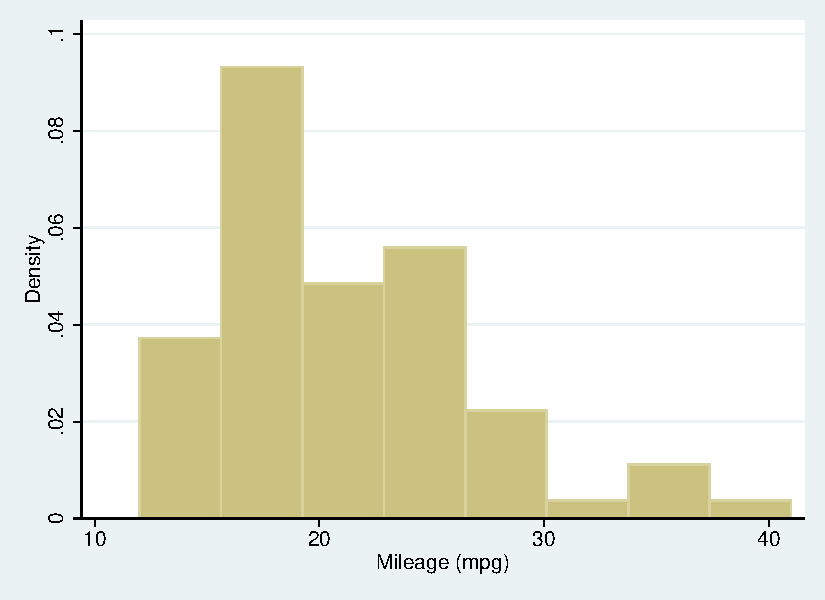
\includegraphics[width=0.4\textwidth]{mod311.pdf}
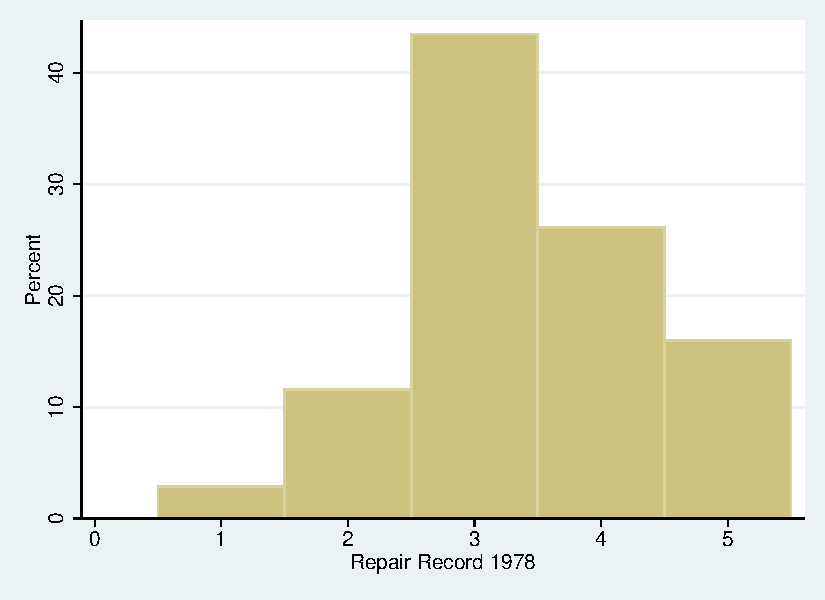
\includegraphics[width=0.4\textwidth]{mod312.pdf}
\caption{\lstinline{histogram}, the right graph with option \lstinline{discrete}\label{histogram}}
\end{figure}

If you are creating a histogram for a categorical variable such as rep78,  you can add the option \lstinline{discrete}. As you can see below, when you specify this option, the midpoint of each bin labels the respective bar.

\begin{lstlisting}
hist rep78, percent discrete
\end{lstlisting}

The \lstinline{graph} \lstinline{box} command can be used to produce a boxplot which can help you examine the distribution of \textit{mpg}. If \textit{mpg} were normally distributed, the line (the median) would be in the middle of the box (the 25th and 75th percentiles, Q1 and Q3) and the ends of the whiskers (the upper and lower adjacent values, which are the most extreme values within Q3+1.5(Q3-Q1) and Q1-1.5*(Q3-Q1), respectively) would be equidistant from the box. The boxplot for \textit{mpg} shows positive skew. The median is pulled to the low end of the box.

\begin{lstlisting}
graph box mpg
\end{lstlisting}

\begin{figure}[!htbp]
\centering
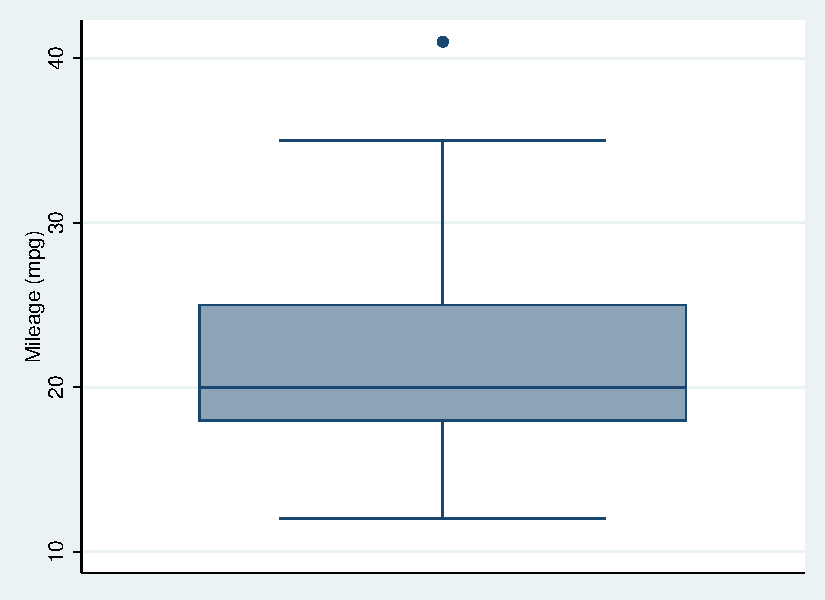
\includegraphics[width=0.4\textwidth]{mod313.pdf}
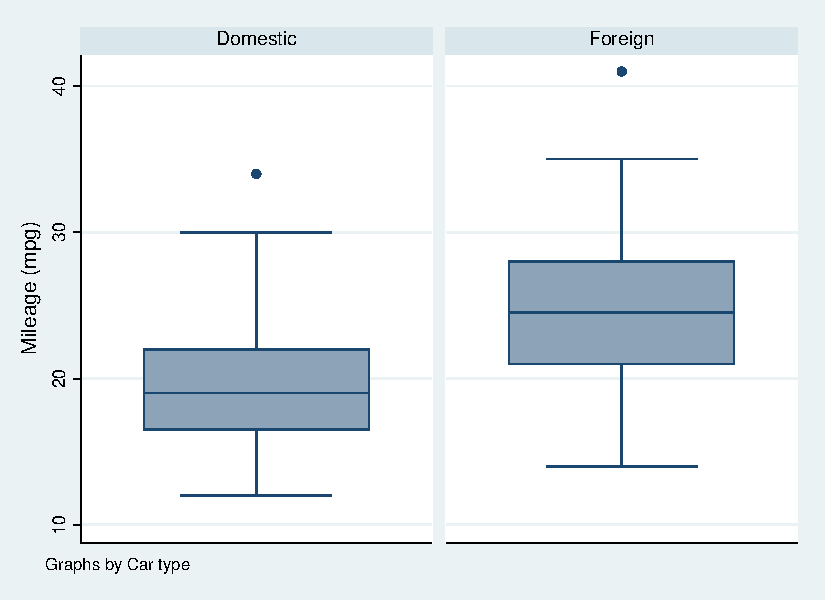
\includegraphics[width=0.4\textwidth]{mod314.pdf}
\caption{\lstinline{graph box}, the right graph with option \lstinline{by}\label{box}}
\end{figure}

The boxplot can be done separately for foreign and domestic cars using the\lstinline{ by( )} or \lstinline{over( )} option.

\begin{lstlisting}
graph box mpg, by(foreign)
\end{lstlisting}

\begin{lstlisting}
graph box mpg, over(foreign)
\end{lstlisting}

As you can see in the graph above, there are a pair of outliers in the box plots produced. These can be removed from the box plot using the \lstinline{noout} command in Stata.

\begin{lstlisting}
graph box mpg, over(foreign) noout
\end{lstlisting}

\begin{figure}[!htbp]
\centering
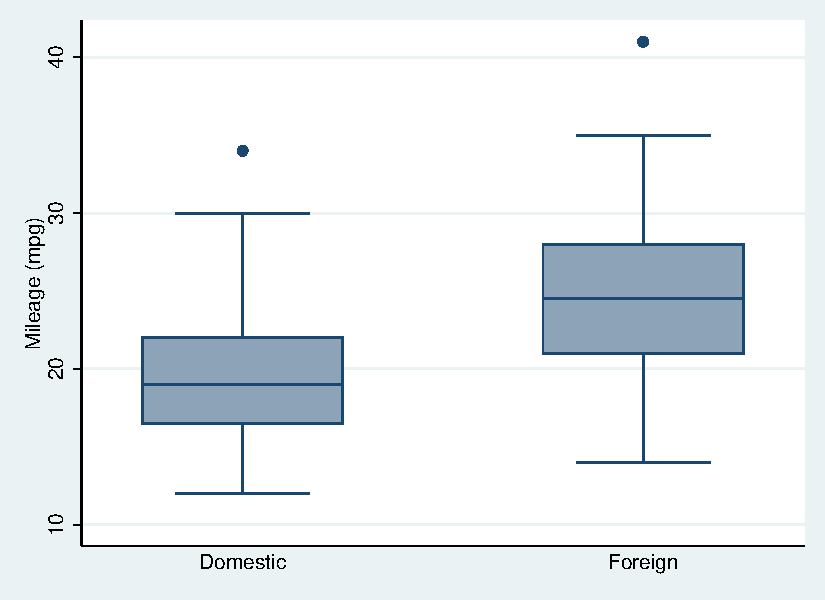
\includegraphics[width=0.4\textwidth]{mod315.pdf}
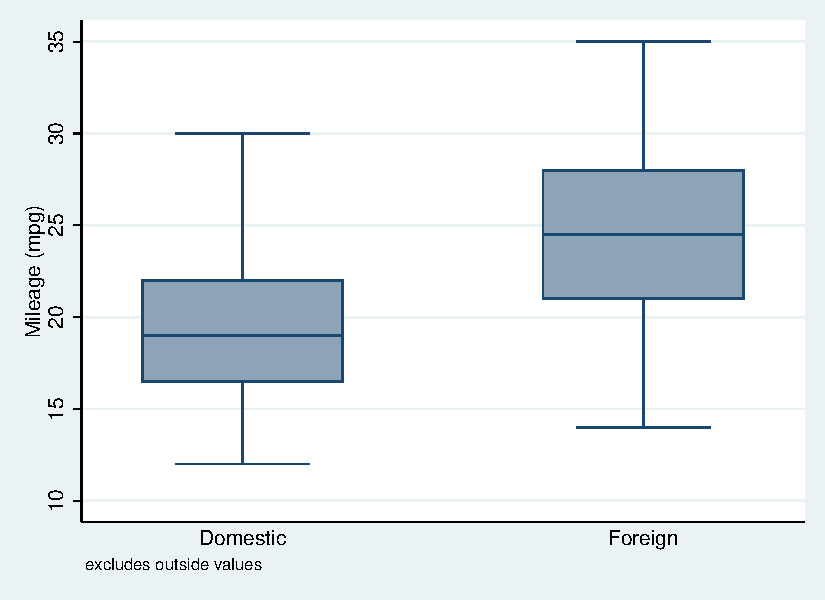
\includegraphics[width=0.4\textwidth]{mod316.pdf}
\caption{\lstinline{graph box} with \lstinline{over}, the right graph with option \lstinline{noout}\label{box2}}
\end{figure}

The graph no longer includes the outlying values. Stata also includes a message at the bottom of the graph noting that outside values were excluded.

Stata can also produce pie charts.

\begin{lstlisting}
graph pie, over(rep78) plabel(_all name) title("Repair Record 1978")
\end{lstlisting}

\begin{center}
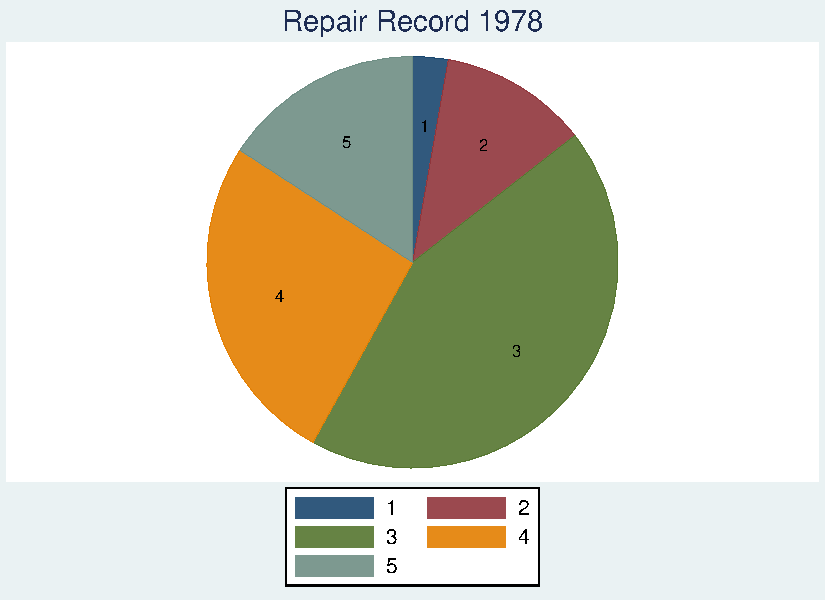
\includegraphics[width=0.4\textwidth]{mod317.pdf}
\end{center}

The \lstinline{graph pie} command with the \lstinline{over} option creates a pie chart representing the frequency of each group or value of \textit{rep78}. The \lstinline{plabel} option places the value labels for \textit{rep78} inside each slice of the pie chart.

A two way scatter plot can be used to show the relationship between \textit{mpg} and \textit{weight}. As we would expect, there is a negative relationship between \textit{mpg} and \textit{weight}.

\begin{lstlisting}
graph twoway scatter mpg weight
\end{lstlisting}

\begin{figure}[!htbp]
\centering
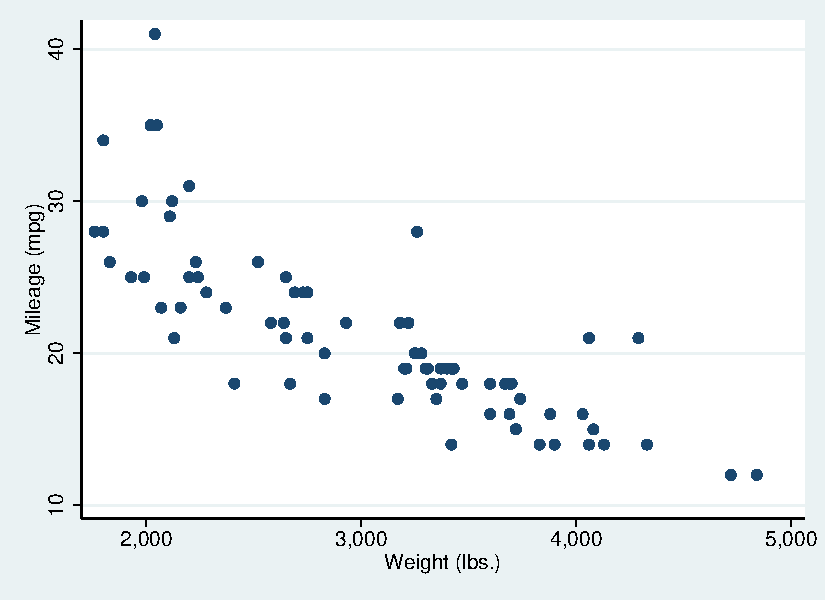
\includegraphics[width=0.4\textwidth]{mod318.pdf}
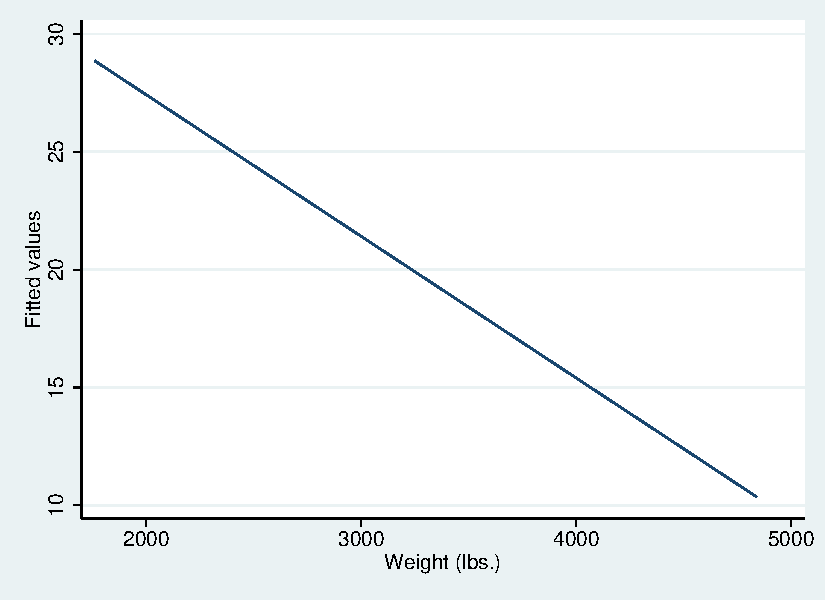
\includegraphics[width=0.4\textwidth]{mod319.pdf}
\caption{\lstinline{twoway graph}, the left graph is \lstinline{scatter} and the right is \lstinline{lfit}\label{twoway}}
\end{figure}

Note that you can save typing like this

\begin{lstlisting}
twoway scatter mpg weight
\end{lstlisting}

We can show the regression line predicting mpg from weight like this.

\begin{lstlisting}
twoway lfit mpg weight
\end{lstlisting}


We can combine these graphs like shown below.

\begin{lstlisting}
twoway (scatter mpg weight) (lfit mpg weight)
\end{lstlisting}

\begin{center}
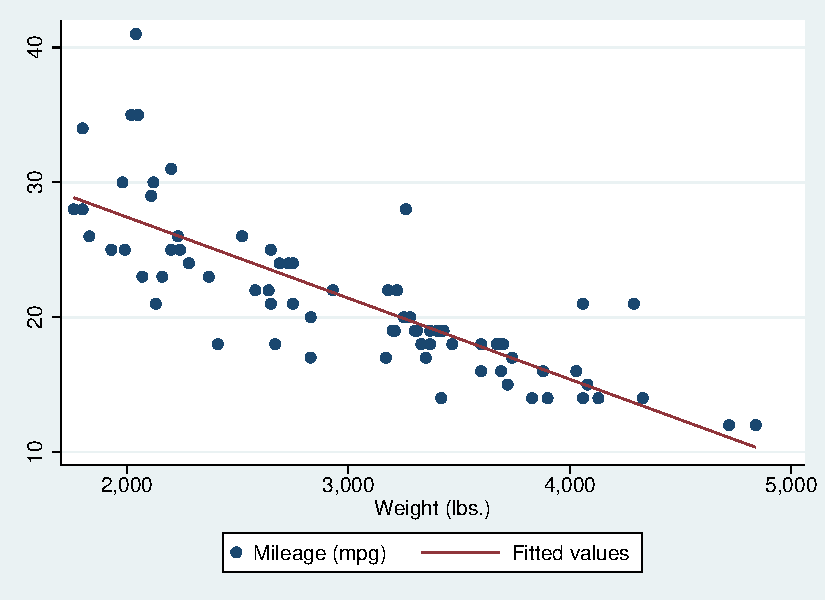
\includegraphics[width=0.4\textwidth]{mod3110.pdf}
\end{center}

We can add labels to the points labeling them by make as shown below. Note that mlabel is an option on the scatter command.

\begin{lstlisting}
twoway (scatter mpg weight, mlabel(make) ) (lfit mpg weight)
\end{lstlisting}


The marker label position can be changed using the \lstinline{mlabangle( )} option.

\begin{lstlisting}
twoway (scatter mpg weight, mlabel(make) mlabangle(45)) (lfit mpg weight)
\end{lstlisting}

\begin{figure}[!h]
\centering
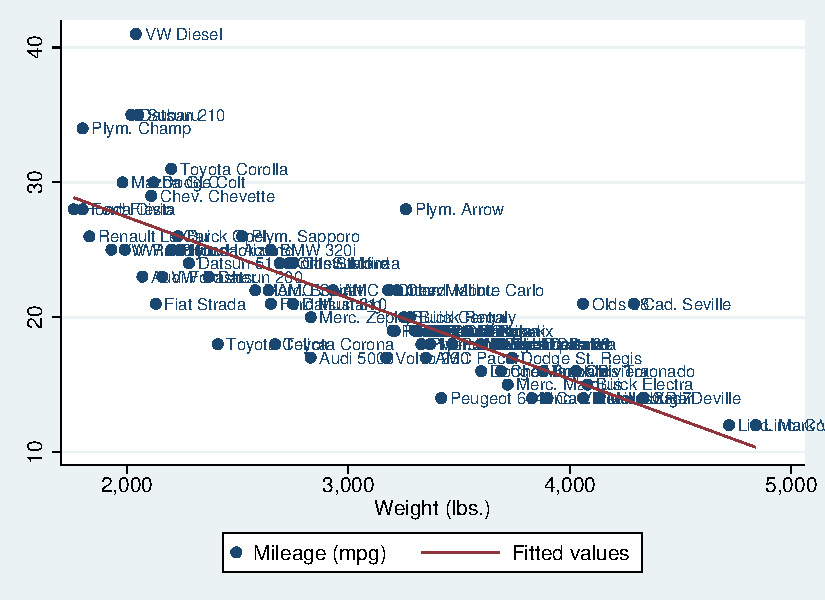
\includegraphics[width=0.4\textwidth]{mod3111.pdf}
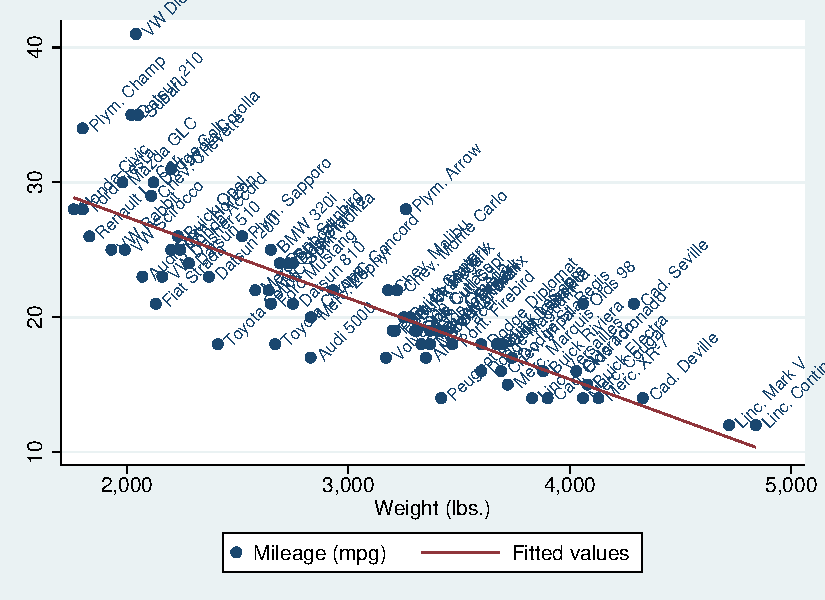
\includegraphics[width=0.4\textwidth]{mod3112.pdf}
\caption{\lstinline{twoway graph mlabel}, the right graph with option \lstinline{mlabangle}\label{twowayx}}
\end{figure}


We can combine separate graphs for foreign and domestic cars as shown below, and we have requested confidence bands around the predicted values by using \lstinline{lfitci} in place of \lstinline{lfit} .  Note that the \lstinline{by} option is at the end of the command.

\begin{lstlisting}
twoway (scatter mpg weight) (lfitci mpg weight), by(foreign)
\end{lstlisting}

You can request a scatter plot matrix with the \lstinline{graph matrix} command. Here we examine the relationships among \textit{mpg}, \textit{weight} and \textit{price}.

\begin{lstlisting}
graph matrix mpg weight price
\end{lstlisting}

\begin{figure}[!htbp]
\centering
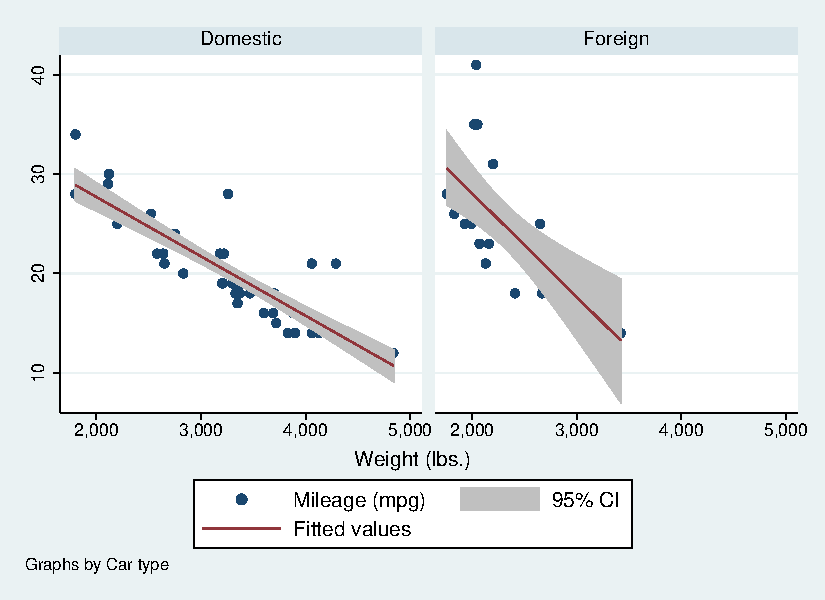
\includegraphics[width=0.4\textwidth]{mod3113.pdf}
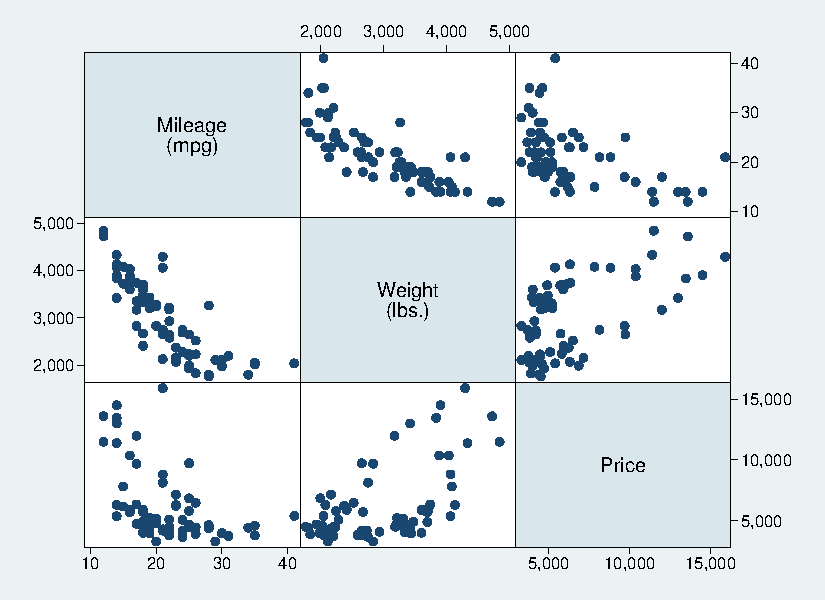
\includegraphics[width=0.4\textwidth]{mod3114.pdf}
\caption{\lstinline{twoway graph with lfitci and graph matrix}\label{twowayxx}}
\end{figure}


\subsection{Graphics: Overview of Twoway Plots}
This module shows examples of the different kinds of graphs that can be created with the \lstinline{graph twoway} command.  This is illustrated by showing the command and the resulting graph.  For more information, see the \href{http://www.stata.com/help.cgi?graph}{Stata Graphics Manual} available over the web and from within Stata by typing \lstinline{help graph}, and in particular the section on \href{http://www.stata.com/help.cgi?scatter}{Two Way Scatterplots}.

\textbf{Basic twoway scatterplot V.S. Line Plot}
\begin{lstlisting}
sysuse sp500
graph twoway scatter close date // the left graph
graph twoway line close date    // the right graph
\end{lstlisting}
\begin{center}
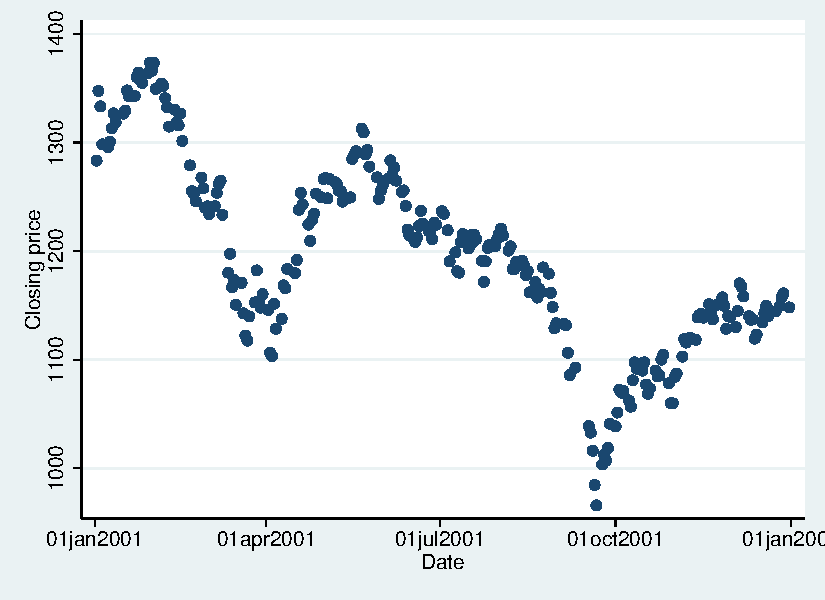
\includegraphics[width=0.4\textwidth]{mod321.pdf}
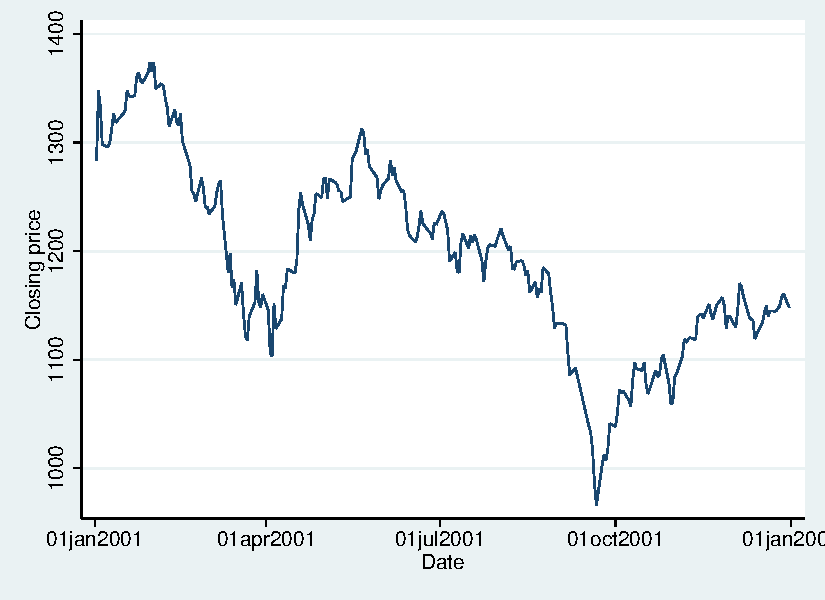
\includegraphics[width=0.4\textwidth]{mod322.pdf}
\end{center}

\textbf{Connected Line Plot}
\begin{lstlisting}
graph twoway connected close date
\end{lstlisting}


\textbf{Immediate scatterplot}
\begin{lstlisting}
graph twoway scatteri ///
  965.8    15239 (3) "Low   965.8" ///
  1373.73  15005 (3) "High 1373.73" , msymbol(i)
\end{lstlisting}

\textbf{Scatterplot and Immediate Scatterplot}
\begin{lstlisting}
graph twoway ///
  (scatter close date) ///
  (scatteri  965.8  15239 (3) "Low, 9/21, 965.8" ///
            1373.7  15005 (3) "High, 1/30, 1373.7", msymbol(i) )
\end{lstlisting}
\begin{center}
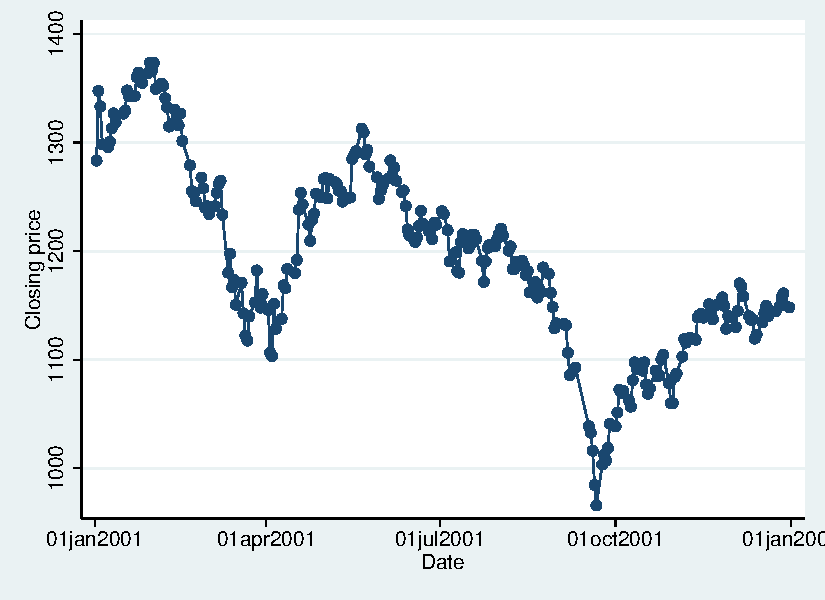
\includegraphics[width=0.33\textwidth]{mod323.pdf}\hfil
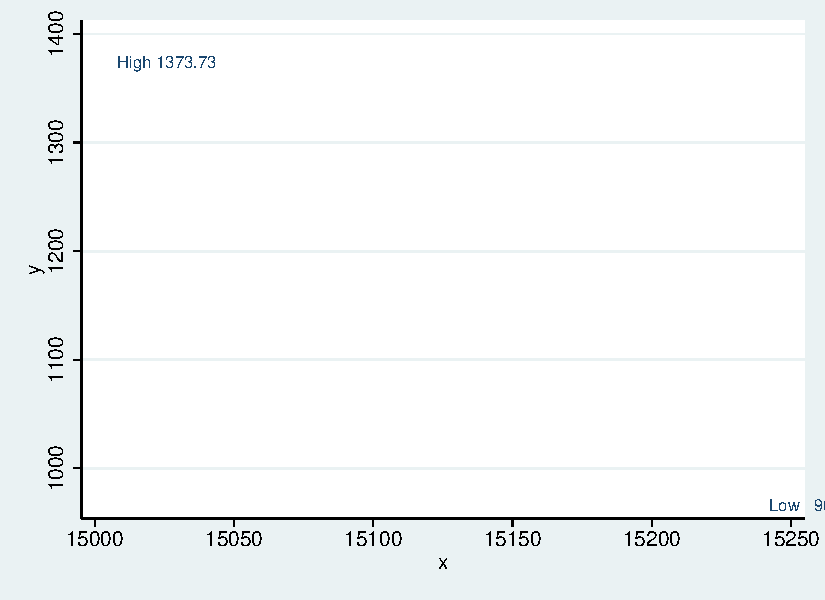
\includegraphics[width=0.33\textwidth]{mod324.pdf}\hfil
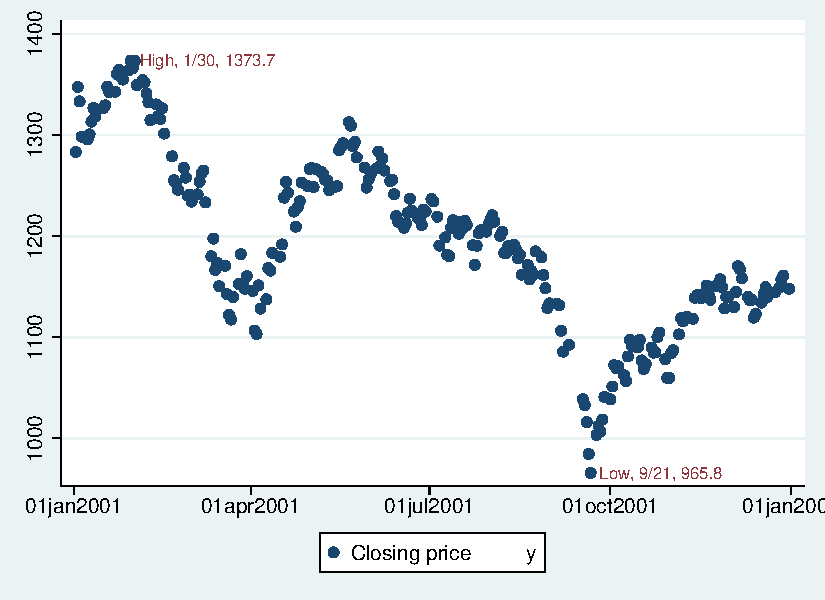
\includegraphics[width=0.33\textwidth]{mod325.pdf}\\
Left graph is twoway scatter plot; the center is the immediate scatter plot; the right is the combination of the two.
\end{center}

\textbf{Area Graph}
\begin{lstlisting}
drop if _n > 57
graph twoway area close date, sort
\end{lstlisting}

\textbf{Bar plot}
\begin{lstlisting}
graph twoway bar close date
\end{lstlisting}

\textbf{Spike plot}
\begin{lstlisting}
graph twoway spike close date
\end{lstlisting}

\textbf{Dropline plot}
\begin{lstlisting}
graph twoway dropline close date
\end{lstlisting}

\begin{center}
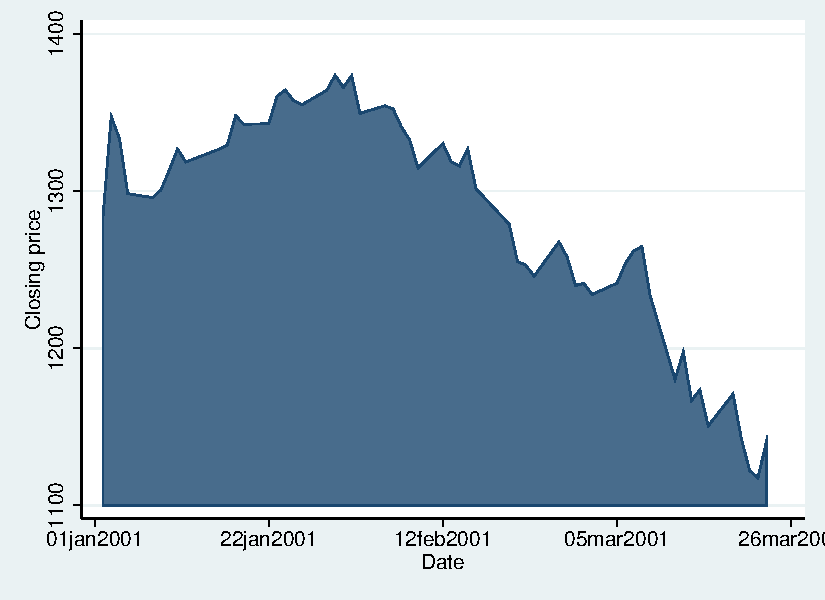
\includegraphics[width=0.40\textwidth]{mod326.pdf}
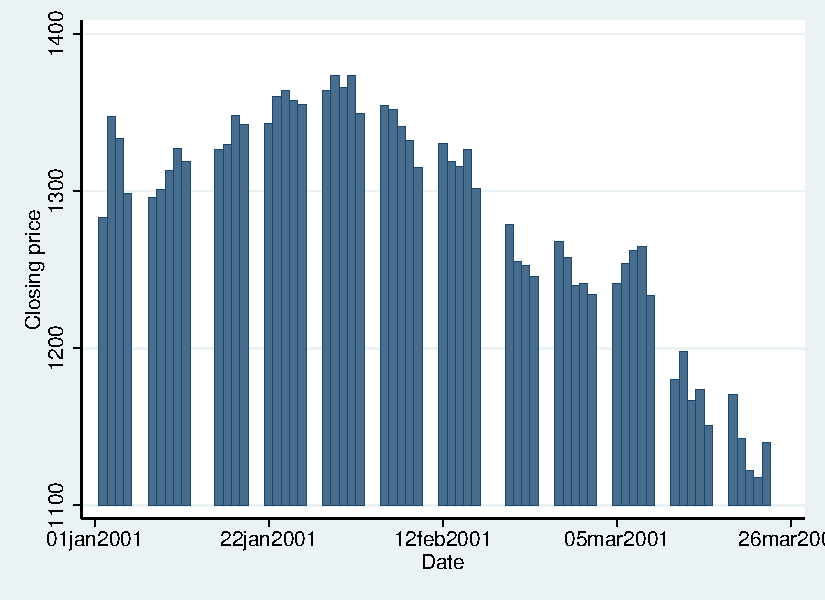
\includegraphics[width=0.40\textwidth]{mod327.pdf}\\
\textbf{Notes:} The left plot is \lstinline{area} plot; the right one is \lstinline{bar} plot.\\
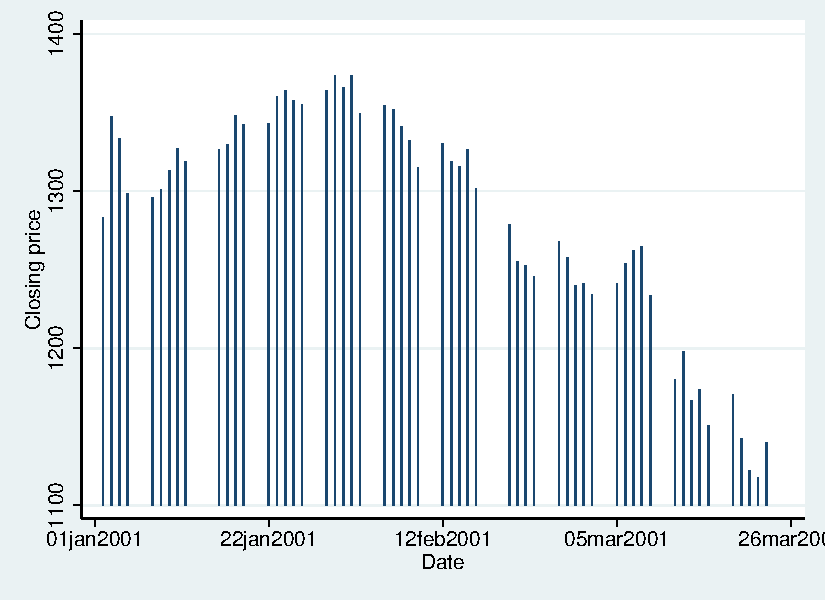
\includegraphics[width=0.40\textwidth]{mod328.pdf}
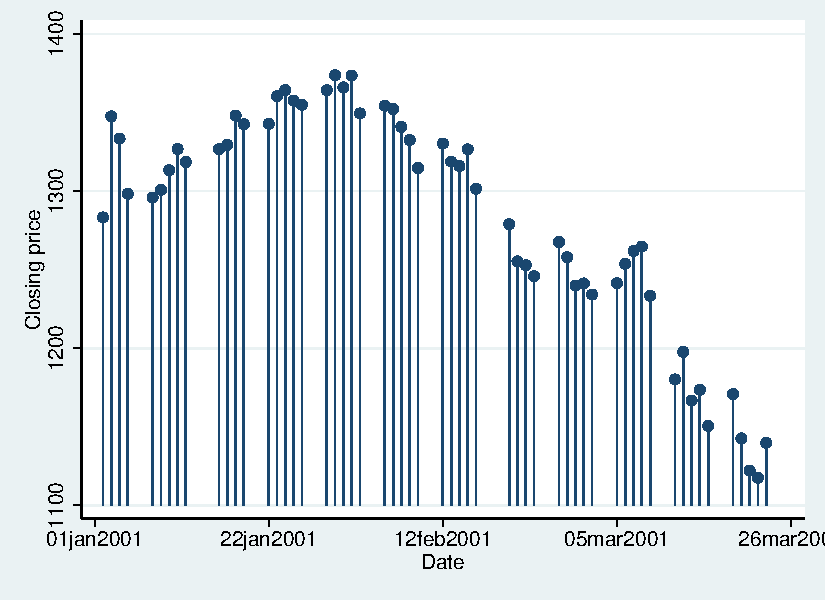
\includegraphics[width=0.40\textwidth]{mod329.pdf}\\
\textbf{Notes:} The left plot is \lstinline{spike} plot; the right one is \lstinline{dropline} plot.\\
\end{center}

\textbf{Dot plot}
\begin{lstlisting}
graph twoway dot change date
\end{lstlisting}

\textbf{Range plot with area shading}
\begin{lstlisting}
graph twoway rarea high low date
\end{lstlisting}

\textbf{Range plot with bars}
\begin{lstlisting}
graph twoway rbar high low date
\end{lstlisting}

\begin{center}
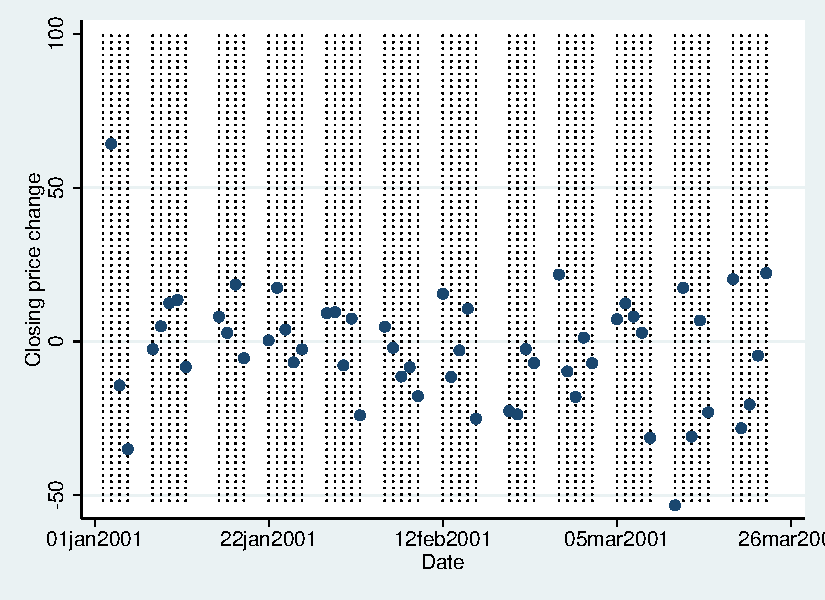
\includegraphics[width=0.33\textwidth]{mod3210.pdf}
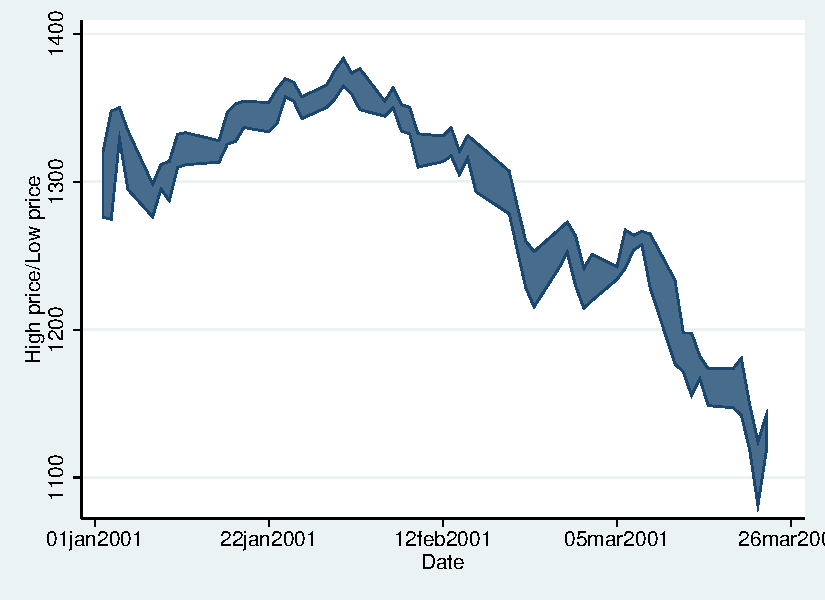
\includegraphics[width=0.33\textwidth]{mod3211.pdf}
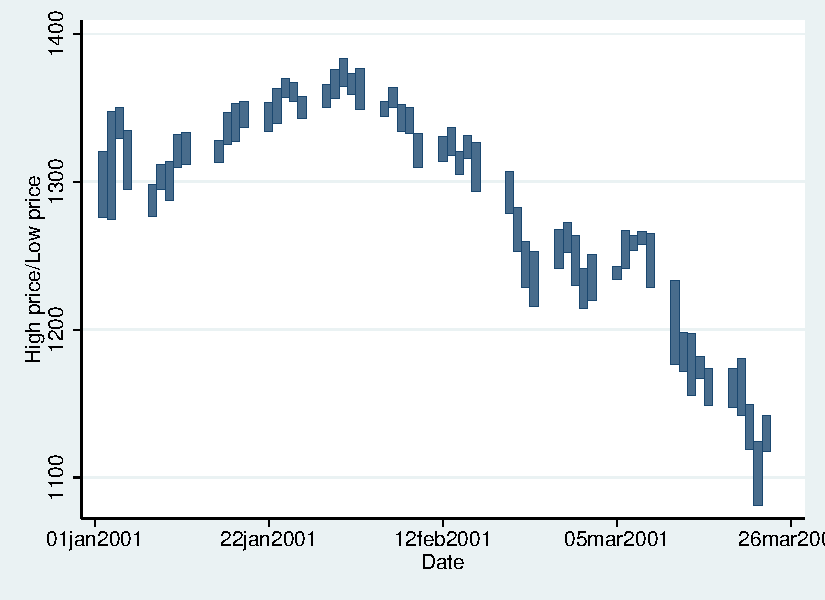
\includegraphics[width=0.33\textwidth]{mod3212.pdf}\\
Left graph is \lstinline{dot} plot; the center is \lstinline{rarea} plot; the right is \lstinline{rbar} plot.
\end{center}

\textbf{Range plot with spikes}
\begin{lstlisting}
graph twoway rspike high low date
\end{lstlisting}

\textbf{Range plot with capped spikes}
\begin{lstlisting}
graph twoway rcap high low date
\end{lstlisting}

\textbf{Range plot with spikes capped with symbols}
\begin{lstlisting}
graph twoway rcapsym high low date
\end{lstlisting}

\begin{center}
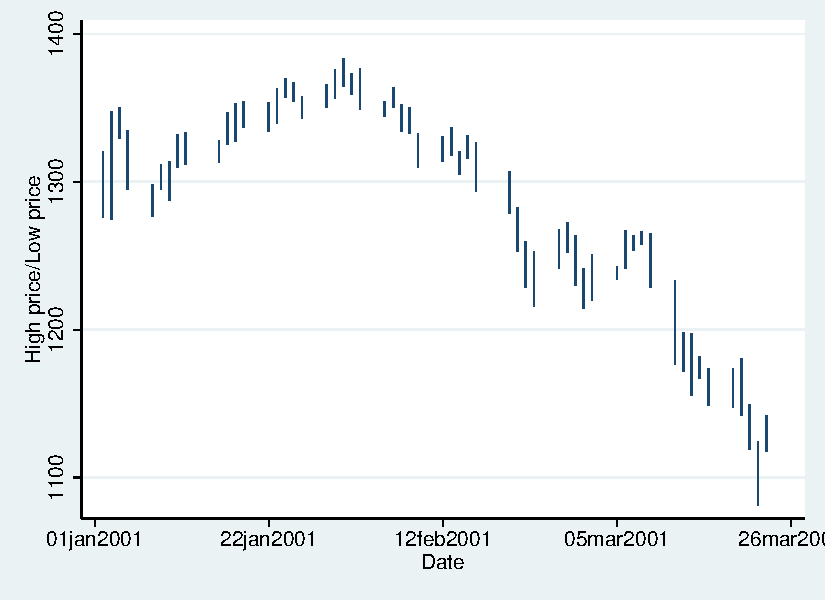
\includegraphics[width=0.33\textwidth]{mod3213.pdf}
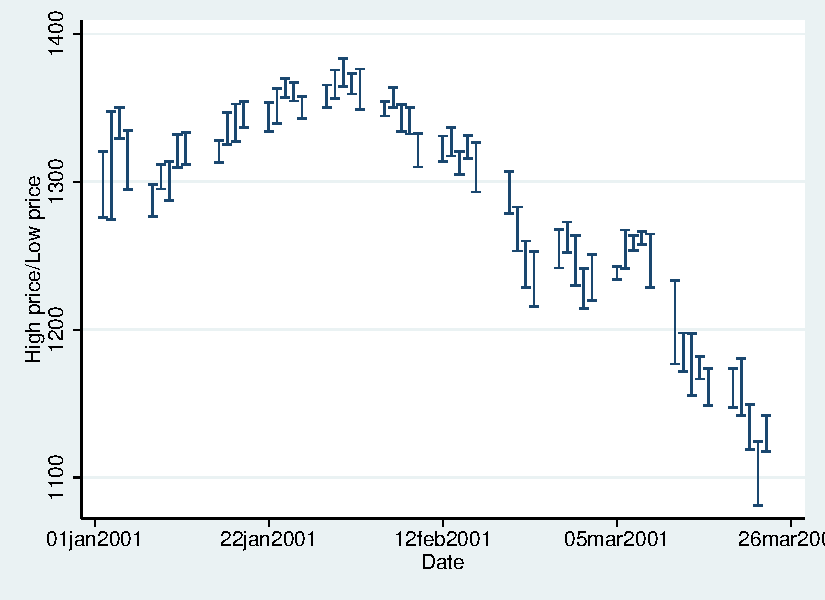
\includegraphics[width=0.33\textwidth]{mod3214.pdf}
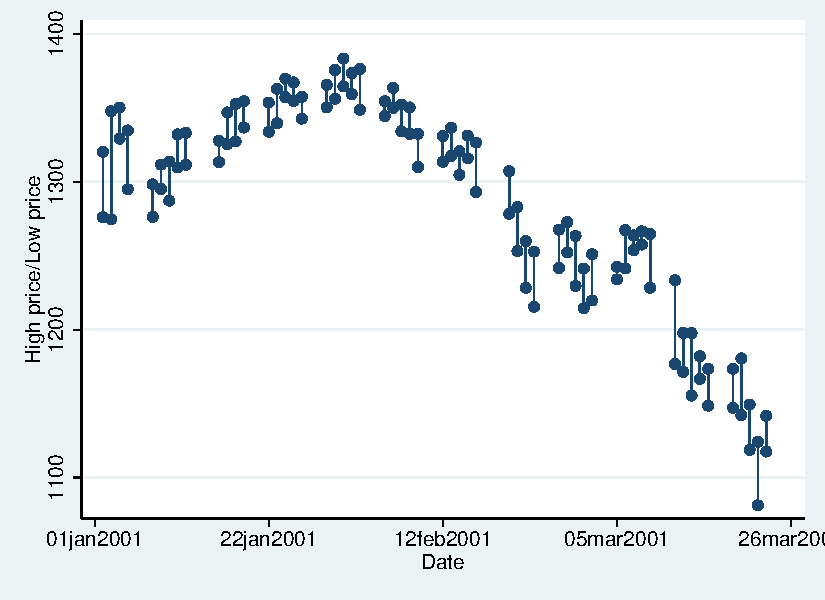
\includegraphics[width=0.33\textwidth]{mod3215.pdf}\\
Left graph is \lstinline{rspike} plot; the center is \lstinline{rcap} plot; the right is \lstinline{rcapsym} plot.
\end{center}

\textbf{Range plot with markers}
\begin{lstlisting}
graph twoway rscatter high low date
\end{lstlisting}

\textbf{Range plot with lines}
\begin{lstlisting}
graph twoway rline high low date
\end{lstlisting}

\textbf{Range plot with lines and markers}
\begin{lstlisting}
graph twoway rconnected high low date
\end{lstlisting}

\begin{center}
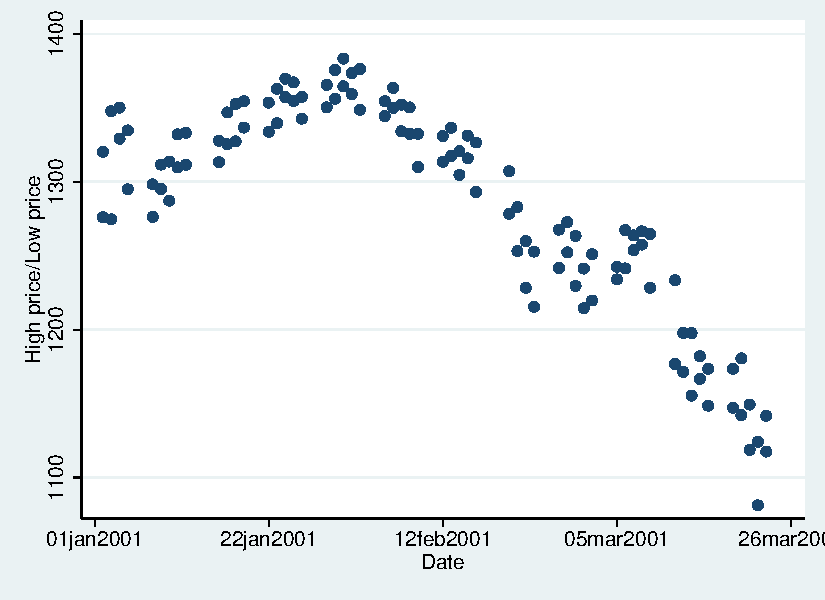
\includegraphics[width=0.33\textwidth]{mod3216.pdf}
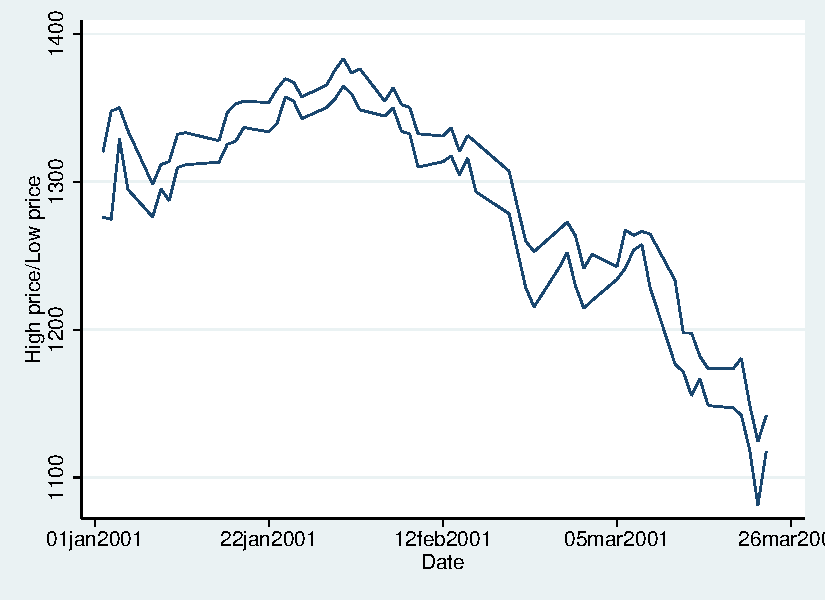
\includegraphics[width=0.33\textwidth]{mod3217.pdf}
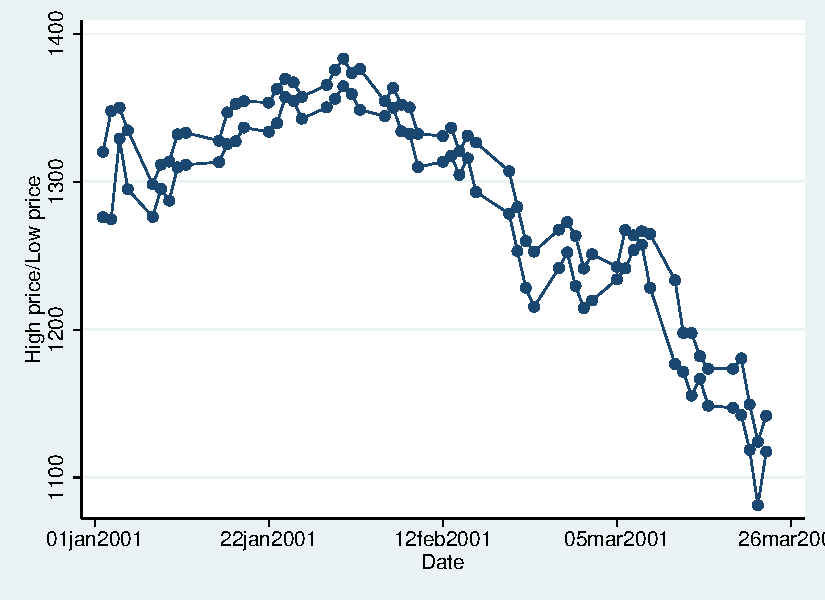
\includegraphics[width=0.33\textwidth]{mod3218.pdf}\\
Left graph is \lstinline{rscatter} plot; the center is \lstinline{rline} plot; the right is \lstinline{rconnected} plot.
\end{center}

% new dataset
\textbf{Median band line plot}
\begin{lstlisting}
use "http://www.ats.ucla.edu/stat/stata/notes/hsb2.dta", clear
graph twoway mband read write
\end{lstlisting}

\textbf{Spline line plot}
\begin{lstlisting}
graph twoway mspline read write
\end{lstlisting}

\textbf{LOWESS line plot}
\begin{lstlisting}
graph twoway lowess read write
\end{lstlisting}

\begin{center}
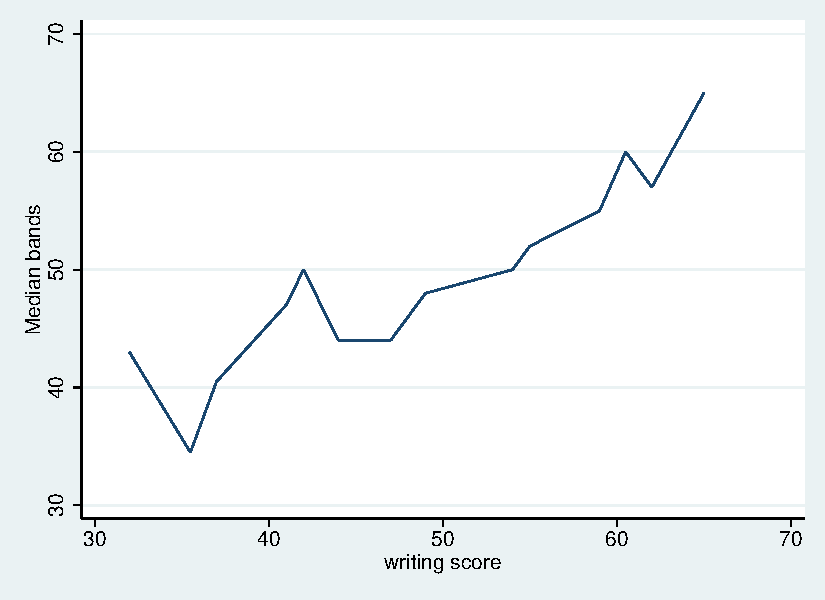
\includegraphics[width=0.33\textwidth]{mod3219.pdf}
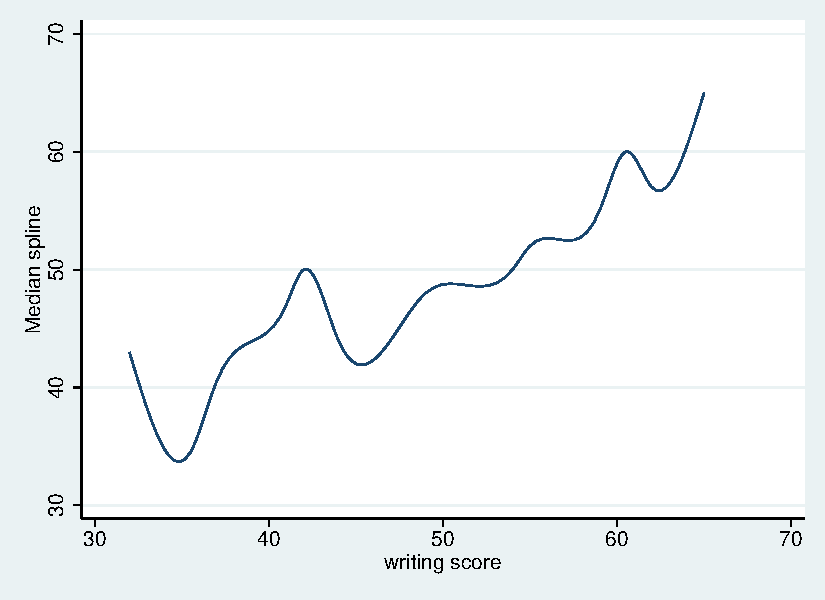
\includegraphics[width=0.33\textwidth]{mod3220.pdf}
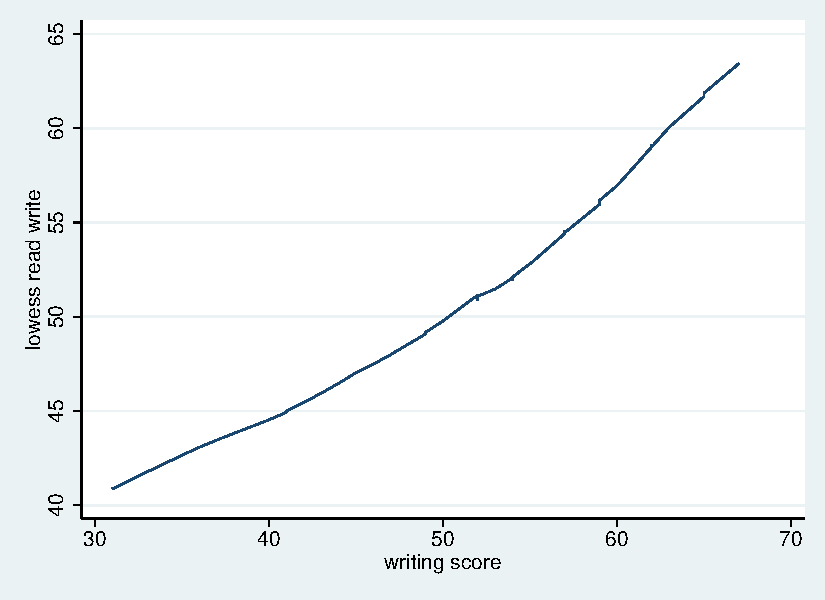
\includegraphics[width=0.33\textwidth]{mod3221.pdf}\\
Left graph is \lstinline{mband} plot; the center is \lstinline{mspline} plot; the right is \lstinline{lowess} plot.
\end{center}


\textbf{Linear prediction plot}
\begin{lstlisting}
graph twoway lfit read write
\end{lstlisting}

\textbf{Quadratic prediction plot}
\begin{lstlisting}
graph twoway qfit read write
\end{lstlisting}

\textbf{Fractional polynomial plot}
\begin{lstlisting}
graph twoway fpfit read write
\end{lstlisting}

\begin{center}
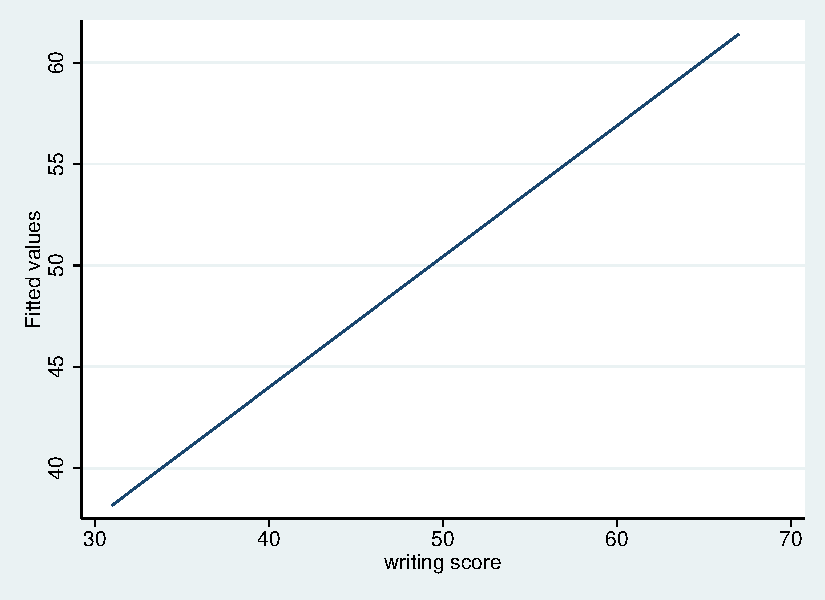
\includegraphics[width=0.33\textwidth]{mod3222.pdf}
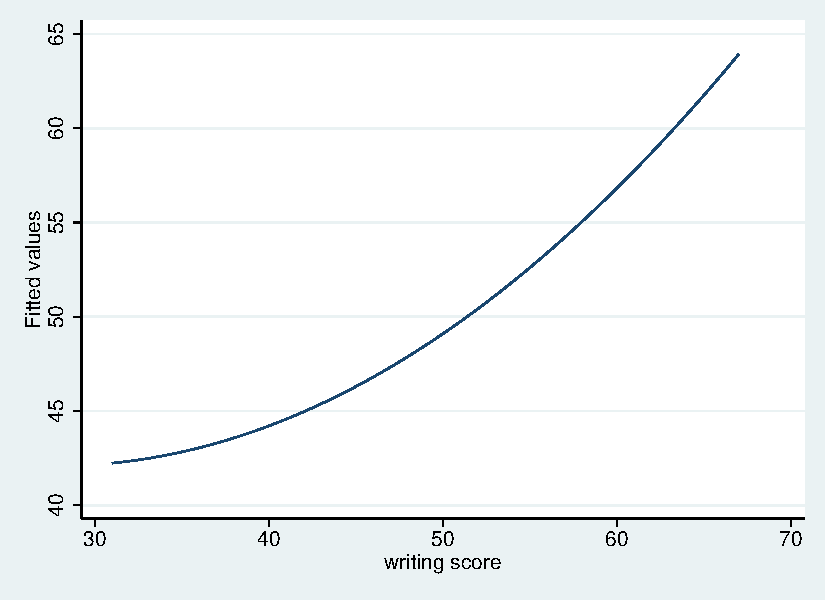
\includegraphics[width=0.33\textwidth]{mod3223.pdf}
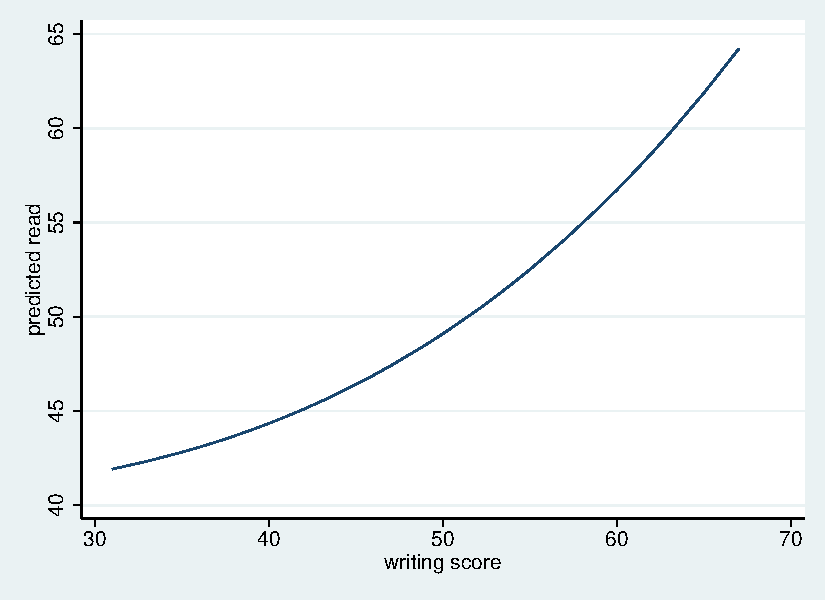
\includegraphics[width=0.33\textwidth]{mod3224.pdf}\\
Left graph is \lstinline{lfit} plot; the center is \lstinline{qfit} plot; the right is \lstinline{fpfit} plot.
\end{center}



\textbf{Linear prediction plot with confidence intervals}
\begin{lstlisting}
graph twoway lfitci read write
\end{lstlisting}

\textbf{Quadratic plot with confidence intervals}
\begin{lstlisting}
graph twoway qfitci read write
\end{lstlisting}

\textbf{Fractional polynomial plot with CIs}
\begin{lstlisting}
graph twoway fpfitci read write
\end{lstlisting}

\begin{center}
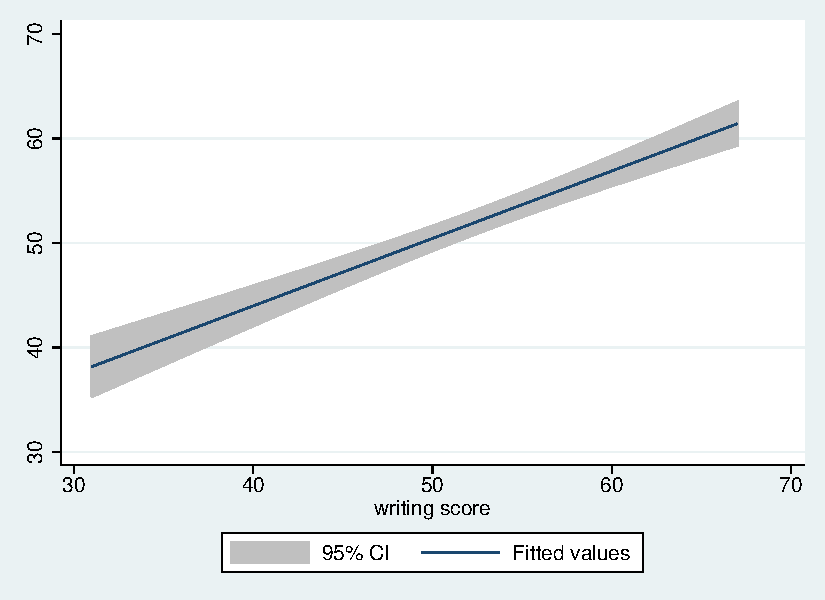
\includegraphics[width=0.33\textwidth]{mod3225.pdf}
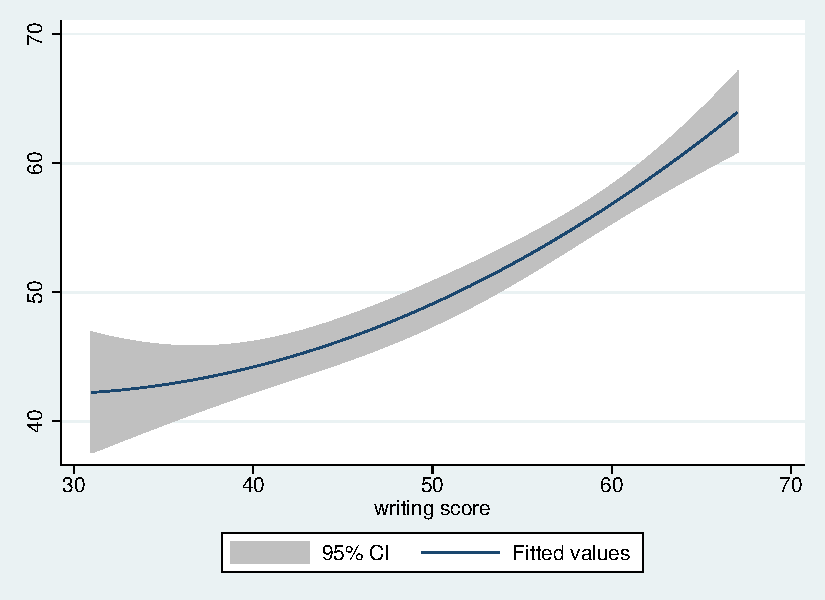
\includegraphics[width=0.33\textwidth]{mod3226.pdf}
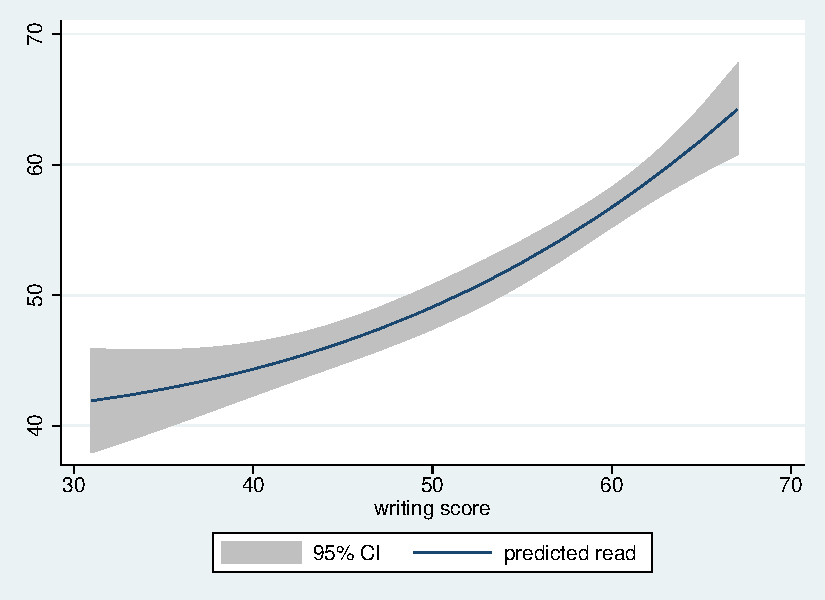
\includegraphics[width=0.33\textwidth]{mod3227.pdf}\\
Left graph is \lstinline{lfitci} plot; the center is \lstinline{qfitci} plot; the right is \lstinline{fpfitci} plot.
\end{center}



\textbf{Histogram}
\begin{lstlisting}
graph twoway histogram read
\end{lstlisting}

\textbf{Kernel density plot}
\begin{lstlisting}
graph twoway kdensity read
\end{lstlisting}

\textbf{Function plot}
\begin{lstlisting}
graph twoway function y=normalden(x), range(-4 4)
\end{lstlisting}
\begin{center}
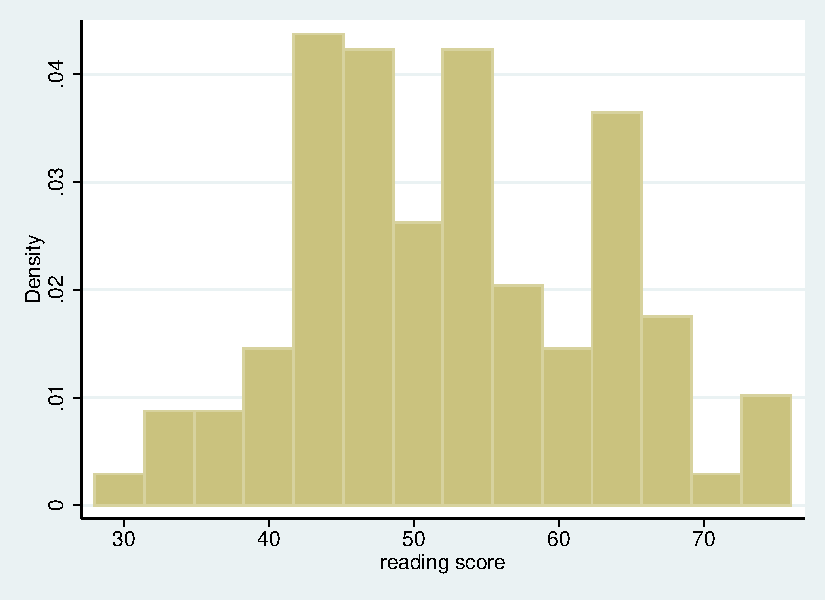
\includegraphics[width=0.33\textwidth]{mod3228.pdf}
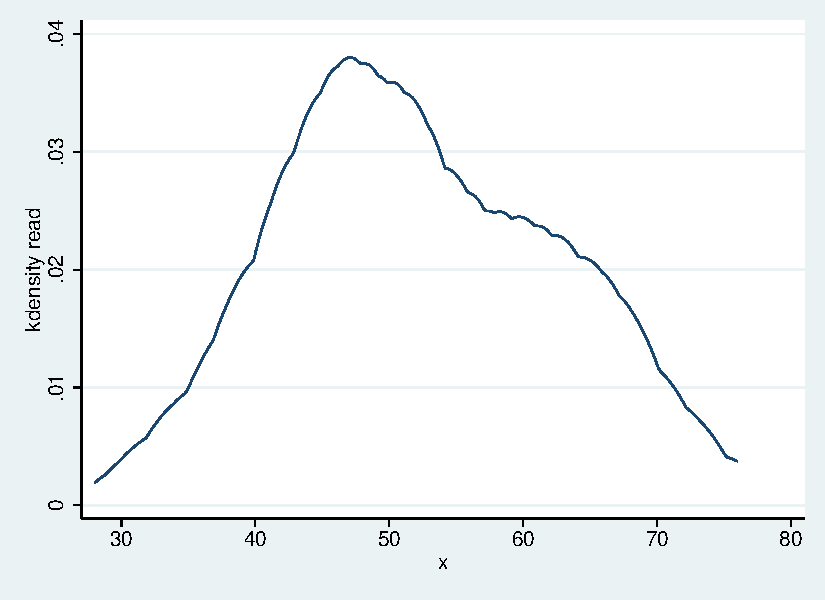
\includegraphics[width=0.33\textwidth]{mod3229.pdf}
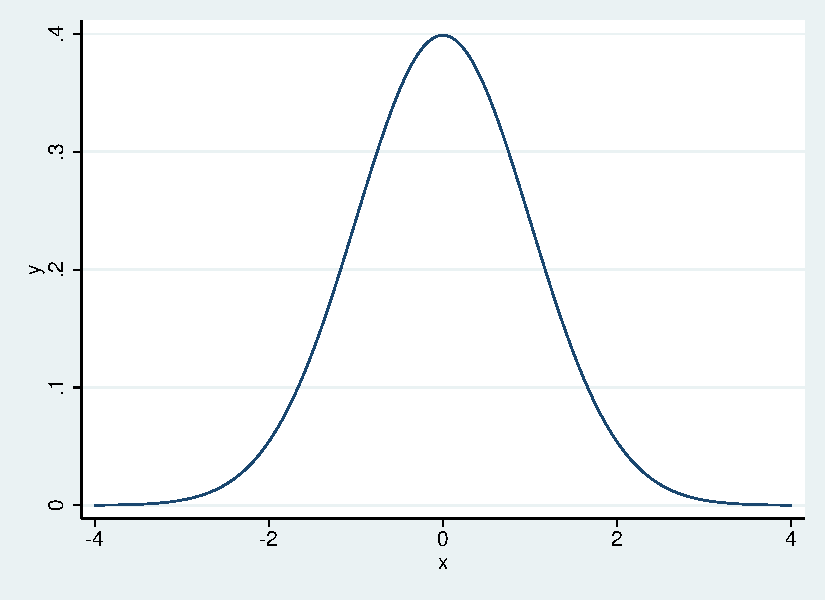
\includegraphics[width=0.33\textwidth]{mod3230.pdf}\\
Left graph is \lstinline{histogram} plot; the center is \lstinline{kdensity} plot; the right is \lstinline{function} plot.
\end{center}


\subsection{Graphics: Twoway Scatterplots}
This module shows some of the options when using the \lstinline{twoway} command to produce scatterplots.  This is illustrated by showing the command and the resulting graph.  This includes hotlinks to the \href{http://www.stata.com/help.cgi?graph}{Stata Graphics Manual} available over the web and from within Stata by typing \lstinline{help graph}.

\subsubsection{Two Way Scatterplots}
\textbf{Basic twoway scatterplot}
\begin{lstlisting}
twoway (scatter read write)
\end{lstlisting}
\begin{center}
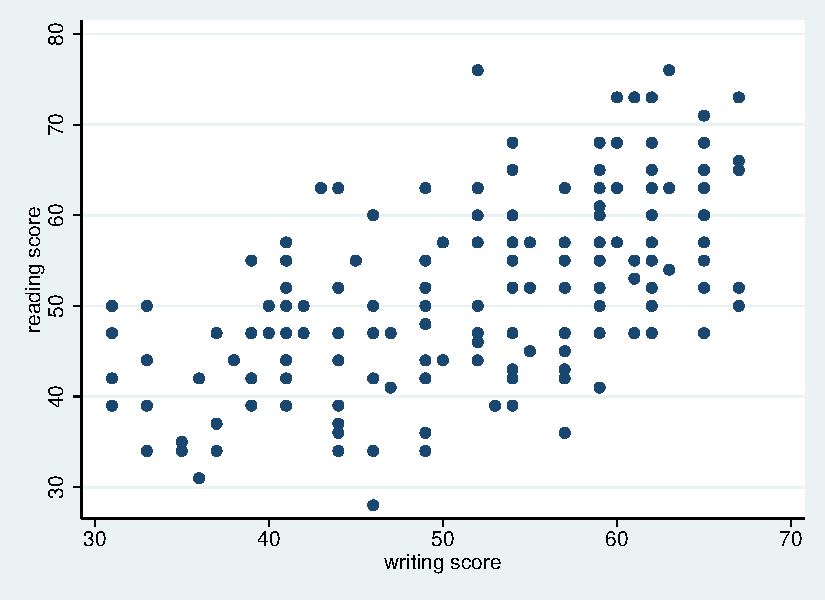
\includegraphics[width=0.5\textwidth]{mod331.pdf}
\end{center}

\subsubsection{Schemes}
\begin{lstlisting}
twoway (scatter read write) , scheme(economist) // use the economist scheme (left)
twoway (scatter read write) , scheme(s1mono)    // use the s1mono scheme (right)
\end{lstlisting}
\begin{center}
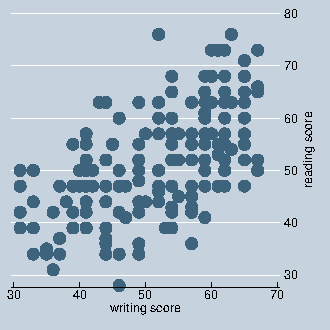
\includegraphics[width=0.35\textwidth]{mod332.pdf}
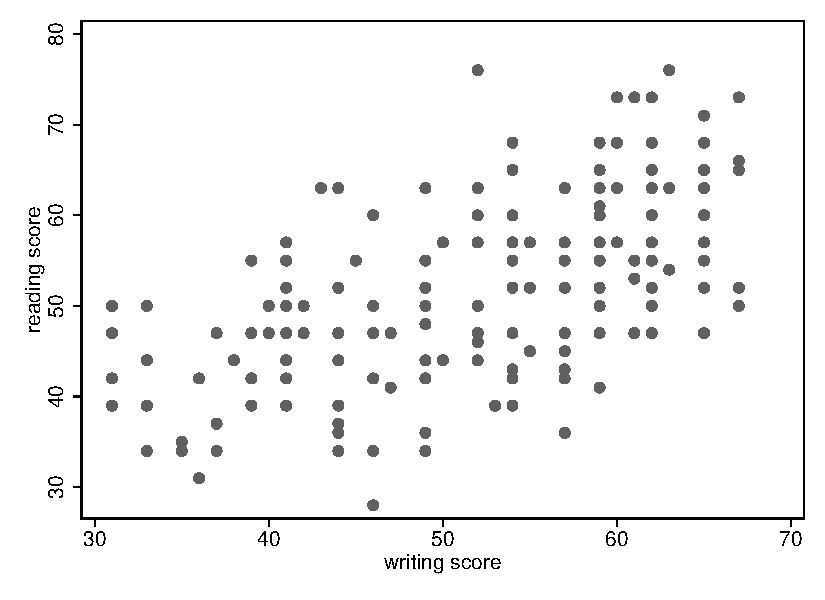
\includegraphics[width=0.49\textwidth]{mod333.pdf}
\end{center}

\subsubsection{Marker Placement Options (i.e. Jitter)}
\begin{lstlisting}
twoway (scatter write read, jitter(3)) // with jitter option (left)
twoway (scatter write read)            // without jitter (right)
\end{lstlisting}
\begin{center}
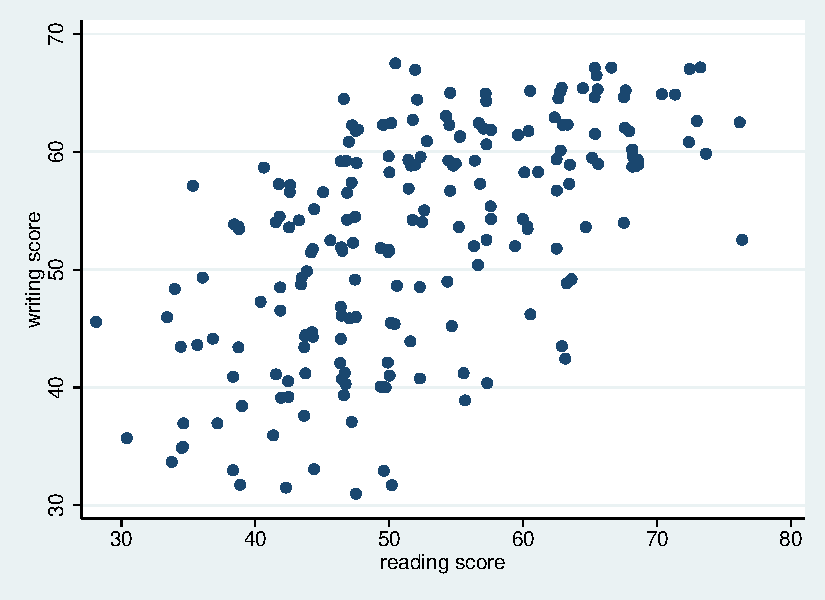
\includegraphics[width=0.42\textwidth]{mod334.pdf}
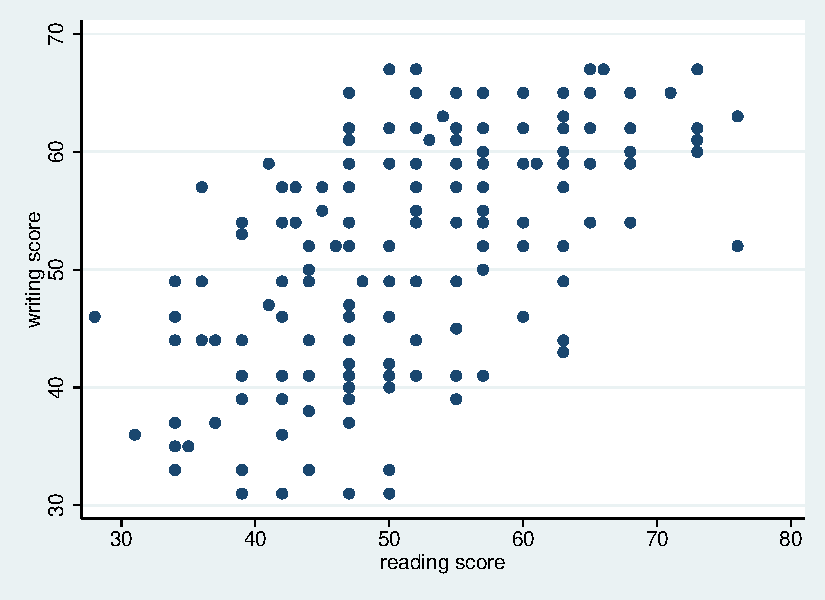
\includegraphics[width=0.42\textwidth]{mod335.pdf}
\end{center}

\subsubsection{Marker Label Options}
\begin{lstlisting}
// Using small black square symbols.
twoway (scatter write read, msymbol(square) msize(small) mcolor(black))
// With markers red on the inside, black medium thick outline
twoway (scatter write read, mfcolor(red) mlcolor(black) mlwidth(medthick))
\end{lstlisting}
\begin{center}
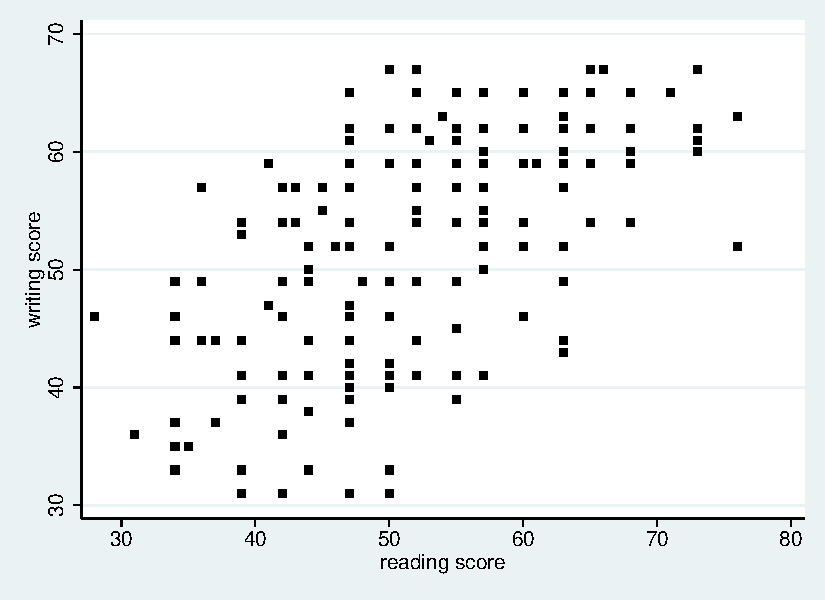
\includegraphics[width=0.42\textwidth]{mod336.pdf}
\includegraphics[width=0.42\textwidth]{mod337.pdf}
\end{center}

\begin{lstlisting}
// Identifying Observations with Marker Labels
twoway (scatter read write, mlabel(id))
// Using large red marker labels at 12 O'clock
twoway (scatter read write if id <=10, mlabel(id) mlabposition(12) mlabsize(large) mlabcolor(red))
\end{lstlisting}
\begin{center}
\includegraphics[width=0.42\textwidth]{mod338.pdf}
\includegraphics[width=0.42\textwidth]{mod339.pdf}
\end{center}

\begin{lstlisting}
// Markers at 90 degree angle at 12 O'clock with a gap of 5
twoway (scatter read write if id <=10, mlabel(ses) mlabangle(90) mlabposition(12) mlabgap(5))
// If mlabgap option is omitted
twoway (scatter read write if id <=10, mlabel(ses) mlabangle(90) mlabposition(12))
\end{lstlisting}
\begin{center}
\includegraphics[width=0.42\textwidth]{mod3310.pdf}
\includegraphics[width=0.42\textwidth]{mod3311.pdf}
\end{center}


\begin{lstlisting}
// Modifying marker position separately for variables (1)
generate pos = 3
replace pos = 1 if (id == 5)
replace pos = 5 if (id == 6)
replace pos = 9 if (id == 3)
twoway (scatter read write if id <= 10, mlabel(ses) mlabv(pos))
// If option mlabv is not used
twoway (scatter read write if id <= 10, mlabel(ses))
\end{lstlisting}
\begin{center}
\includegraphics[width=0.40\textwidth]{mod3312.pdf}
\includegraphics[width=0.40\textwidth]{mod3313.pdf}
\end{center}

\subsubsection{Connect Options}

\begin{lstlisting}
// Connecting with straight line
egen mread = mean(read), by(write)
twoway (scatter mread write,connect(l) sort)
// If the sort option is omitted
twoway (scatter mread write,connect(l))
// Thick black dotted connecting line
twoway (scatter mread write,connect(l) clwidth(thick) clcolor(black) clpattern(dot) sort)
\end{lstlisting}
\begin{center}
\includegraphics[width=0.33\textwidth]{mod3314.pdf}
\includegraphics[width=0.33\textwidth]{mod3315.pdf}
\includegraphics[width=0.33\textwidth]{mod3316.pdf}
\end{center}


\begin{lstlisting}
// Show gaps in line when there are missing values
egen sdread = sd(read), by(write)
twoway (scatter sdread write, connect(l) sort cmissing(n))
// Omitting cmissing option
twoway (scatter sdread write, connect(l) sort)
\end{lstlisting}
\begin{center}
\includegraphics[width=0.40\textwidth]{mod3317.pdf}
\includegraphics[width=0.40\textwidth]{mod3318.pdf}
\end{center}

\subsection{Graphics: Combining Twoway Scatterplots}

This module shows examples of combining twoway scatterplots.  This is illustrated by showing the command and the resulting graph.  This includes hotlinks to the \href{http://www.stata.com/help.cgi?graph}{Stata Graphics Manual} available over the web and from within Stata by typing \lstinline{help graph}.

The data set used in these examples can be obtained using the following command:
\begin{lstlisting}
use "http://www.ats.ucla.edu/stat/stata/notes/hsb2.dta", clear
\end{lstlisting}

This illustrates combining graphs in the following situations.
\begin{compactitem}
\item Plots for separate groups (using \lstinline{by})
\item Combining separate plots together into a single plot
\item Combining separate graphs together into a single graph
\end{compactitem}

\subsubsection{Plots for separate groups}

\begin{lstlisting}
// Separate graphs by gender (male and female)
twoway (scatter read write), by(female)
// Separate graphs by ses and gender
twoway (scatter read write), by(female ses)
// Swapping position of ses and gender
twoway (scatter read write), by(ses female, cols(2))
\end{lstlisting}
\begin{center}
\includegraphics[width=0.33\textwidth]{mod341.pdf}
\includegraphics[width=0.33\textwidth]{mod342.pdf}
\includegraphics[width=0.33\textwidth]{mod343.pdf}
\end{center}

\subsubsection{Combining scatterplots and linear fit in one graph}

\begin{lstlisting}
// Scatterplot with linear fit
twoway (scatter read write) ///
       (lfit read write) ,
        ytitle(Reading Score)
// Graphs separated by SES and female with linear fit lines and points identified by id
twoway (scatter read write, mlabel(id)) ///
       (lfit read write, range(30 70)) ,
        ytitle(Reading Score) by(ses female)
// Graph for high ses females with linear fit with and without obs 51
twoway (scatter read write, mlabel(id)) ///
       (lfit read write, range(30 70)) ///
       (lfit read write if id != 51, range(30 70)) if female==1 & ses==3,
        ytitle(Reading Score) legend(lab(3 "Fitted values without Obs 51"))
\end{lstlisting}
\begin{center}
\includegraphics[width=0.33\textwidth]{mod344.pdf}
\includegraphics[width=0.33\textwidth]{mod345.pdf}
\includegraphics[width=0.33\textwidth]{mod346.pdf}
\end{center}

\subsubsection{Combining scatterplots with multiple variables and linear fits}

\begin{lstlisting}
// Reading and math score by writing score
twoway (scatter read write) ///        plot(1,1)
       (scatter math write)
// Reading and math score by writing score with fit lines
twoway (scatter read write) (scatter math write) /// plot(1,2)
       (lfit read write)    (lfit math write)    ///
// Adding legend to above graph
twoway (scatter read write) ///        plot(2,1)
       (scatter math write) ///
       (lfit read write)  ///
       (lfit math write), ///
       legend(label(3 "Linear Fit") label(4 "Linear Fit")) ///
       legend(order(1 3 2 4))
// Final version of graph making line style same as dot style, and ranges the same
twoway (scatter read write) ///        plot(2,2)
       (scatter math write) ///
       (lfit read write, pstyle(p1) range(25 80) )  ///
       (lfit math write, pstyle(p2) range(25 80) ), ///
       legend(label(3 "Linear Fit") label(4 "Linear Fit")) ///
       legend(order(1 3 2 4))
\end{lstlisting}
\begin{center}
\includegraphics[width=0.42\textwidth]{mod347.pdf}
\includegraphics[width=0.42\textwidth]{mod348.pdf}
\includegraphics[width=0.42\textwidth]{mod349.pdf}
\includegraphics[width=0.42\textwidth]{mod3410.pdf}
\end{center}


\subsubsection{Combining scatterplots and linear fit for separate groups}

\begin{lstlisting}
// Overlay graph of males and females in one graph
separate write, by(female)
twoway (scatter write0 read) (scatter write1 read), ///
       ytitle(Writing Score) legend(order(1 "Males" 2 "Females"))
// Overlay graph of males and females in one graph with linear fit lines
twoway (scatter write0 read) (scatter write1 read) ///
     (lfit write0 read) (lfit write1 read), ///
     ytitle(Writing Score) ///
     legend(order(1 "Males" 2 "Females" 3 "Lfit Males" 4 "Lfit Females"))
\end{lstlisting}
\begin{center}
\includegraphics[width=0.42\textwidth]{mod3411.pdf}
\includegraphics[width=0.42\textwidth]{mod3412.pdf}
\end{center}

\subsubsection{Combining separate graphs into one graph}
First, we make 3 graphs (not shown)
\begin{lstlisting}
// Making the Graphs
twoway (scatter read write) (lfit read write), name(scatterx)
regress read write
rvfplot, name(rvf)
lvr2plot, name(lvr)
\end{lstlisting}

Now we can use \lstinline{graph combine} to combine these into one graph, we can also move the place where the empty graph is located, as shown below.

\begin{lstlisting}
// combine the three graphs into one graph
graph combine scatterx rvf lvr
// Combining the graphs differently
graph combine scatterx rvf lvr, hole(2)
\end{lstlisting}
\begin{center}
\includegraphics[width=0.42\textwidth]{mod3413.pdf}
\includegraphics[width=0.42\textwidth]{mod3414.pdf}
\end{center}

\subsection{Graphics: Common Graph Options}
This module shows examples of the different kinds of graphs that can be created with the \lstinline{graph twoway} command.  This is illustrated by showing the command and the resulting graph.  For more information, see the \href{http://www.stata.com/help.cgi?graph}{Stata Graphics Manual} available over the web and from within Stata by typing \lstinline{help graph}, and in particular the section on \textit{Two Way Scatterplots}.

\begin{lstlisting}
// Adding a title
graph twoway scatter read write, ///
  title("Scatterplot of Reading and Writing")
// Black title, positioned at 11 O'Clock
graph twoway scatter read write, ///
  title("Scatterplot of Reading and Writing", ///
  color(black) position(11))
// Title at 5 O'Clock, medium size text, positioned within the graph
graph twoway scatter read write, ///
  title("Scatterplot of Reading and Writing", ///
  size(medium) position(5) ring(0))
\end{lstlisting}
\begin{center}
\includegraphics[width=0.33\textwidth]{mod351.pdf}
\includegraphics[width=0.33\textwidth]{mod352.pdf}
\includegraphics[width=0.33\textwidth]{mod353.pdf}
\end{center}

\begin{lstlisting}
// Title in a box with cyan background, magenta border and a medium margin around the title
graph twoway scatter read write, ///
  title("Scatterplot of Reading and Writing", ///
         box bcolor(cyan) blcolor(magenta) bmargin(medium))
// Two line title with a gap of 3 between the titles
graph twoway scatter read write, ///
  title("Scatterplot of Reading and Writing" ///
  "Sample of 200 Students", linegap(3) )
\end{lstlisting}

\begin{center}
\includegraphics[width=0.42\textwidth]{mod354.pdf}
\includegraphics[width=0.42\textwidth]{mod355.pdf}
\end{center}

\begin{lstlisting}
// Graph with title, subtitle, caption, and a note
graph twoway scatter read write, ///
  title("Scatterplot of Reading and Writing") ///
  subtitle("Sample of 200 Students") ///
  note(High School and Beyond Data) ///
  caption(From www.ats.ucla.edu)
// Moving and sizing note and caption
graph twoway scatter read write, ///
  title("Scatterplot of Reading and Writing") ///
  subtitle("Sample of 200 Students") ///
  note(High School and Beyond Data, size(medium) position(5)) ///
  caption(From www.ats.ucla.edu, size(vsmall) position(5))
\end{lstlisting}

\begin{center}
\includegraphics[width=0.42\textwidth]{mod356.pdf}
\includegraphics[width=0.42\textwidth]{mod357.pdf}
\end{center}

\begin{lstlisting}
// Modifying title on x and y axis
twoway scatter read write, ///
  ytitle(Score on Writing Test) ///
  xtitle(Score on Reading Test)

// Complete example
twoway scatter read write, ///
  title("Scatterplot of Reading and Writing") ///
  subtitle("Sample of 200 Students") ///
  note(High School and Beyond Data, size(medium) position(5)) ///
  caption(From www.ats.ucla.edu, size(vsmall) position(5)) ///
  ytitle(Score on Writing Test) ///
  xtitle(Score on Reading Test)
\end{lstlisting}
\begin{center}
\includegraphics[width=0.42\textwidth]{mod358.pdf}
\includegraphics[width=0.42\textwidth]{mod359.pdf}
\end{center}

\begin{lstlisting}
// Sizing graph to have 4 by 2 aspect ratio
twoway scatter read write, ysize(2) xsize(4)

// Making text scaled 1.5 times normal size
graph twoway scatter read write, scale(1.5)
\end{lstlisting}

\begin{center}
\includegraphics[width=0.5\textwidth]{mod3510.pdf}
\includegraphics[width=0.42\textwidth]{mod3511.pdf}
\end{center}

\begin{lstlisting}
// Graph with sand color outside graph, gray inside graph
graph twoway scatter read write, ///
  title("Scatterplot of Reading and Writing") ///
  graphregion( color(sand) ) plotregion(  fcolor(gray) )

// Graph with sand color outside graph, gray inside graph, red outer border, blue inner border
graph twoway scatter read write, ///
  title("Scatterplot of Reading and Writing") ///
  graphregion( fcolor(red)  ifcolor(sand) ) ///
  plotregion(  fcolor(blue) ifcolor(gray))

// Graph with colors for many border elements
graph twoway scatter read write, ///
  title("Scatterplot of Reading and Writing") ///
  graphregion( fcolor(red)   lcolor(yellow)  lwidth(thick)  ///
              ifcolor(sand) ilcolor(orange)  ilwidth(thick)) ///
  plotregion(  fcolor(blue)  lcolor(green)   lwidth(thick)  ///
              ifcolor(gray) ilcolor(purple)  ilwidth(thick))
\end{lstlisting}

\begin{center}
\includegraphics[width=0.33\textwidth]{mod3512.pdf}
\includegraphics[width=0.33\textwidth]{mod3513.pdf}
\includegraphics[width=0.33\textwidth]{mod3514.pdf}
\end{center}

\newpage
\section{Reading Data in Stata}
\subsection{Using and saving files in Stata}
\subsubsection{Using and saving Stata data files}

The \lstinline{use} command gets a Stata data file from disk and places it in memory so you can analyze and/or modify it. A data file must be read into memory before you can analyze it. It is kind of like when you open a \textit{Word} document; you need to read a \textit{Word} document into \textit{Word} before you can work with it. The use command below gets the Stata data file called \lstinline{auto.dta} from disk and places it in memory so we can analyze and/or modify it. Since Stata data files end with \lstinline{.dta} you need only say \lstinline{use auto} and Stata knows to read in the file called \lstinline{auto.dta}.

\begin{lstlisting}
sysuse auto
\end{lstlisting}

The \lstinline{describe} command tells you information about the data that is currently sitting in memory.

\begin{lstlisting}
describe

Contains data from auto.dta
  obs:            74
 vars:            12                          17 Feb 1999 10:49
 size:         3,108 (99.6% of memory free)
-------------------------------------------------------------------------------
   1. make      str17  %17s
   2. price     int    %9.0g
   3. mpg       byte   %9.0g
   4. rep78     byte   %9.0g
   5. hdroom    float  %9.0g
   6. trunk     byte   %9.0g
   7. weight    int    %9.0g
   8. length    int    %9.0g
   9. turn      byte   %9.0g
  10. displ     int    %9.0g
  11. gratio    float  %9.0g
  12. foreign   byte   %9.0g
-------------------------------------------------------------------------------
Sorted by:
\end{lstlisting}

Now that the data is in memory, we can analyze it. For example, the \lstinline{summarize} command gives summary statistics for the data currently in memory.

\begin{lstlisting}
summarize

Variable |     Obs        Mean   Std. Dev.       Min        Max
---------+-----------------------------------------------------
    make |       0
   price |      74    6165.257   2949.496       3291      15906
     mpg |      74     21.2973   5.785503         12         41
   rep78 |      69    3.405797   .9899323          1          5
  hdroom |      74    2.993243   .8459948        1.5          5
   trunk |      74    13.75676   4.277404          5         23
  weight |      74    3019.459   777.1936       1760       4840
  length |      74    187.9324   22.26634        142        233
    turn |      74    39.64865   4.399354         31         51
   displ |      74    197.2973   91.83722         79        425
  gratio |      74    3.014865   .4562871       2.19       3.89
 foreign |      74    .2972973   .4601885          0          1
\end{lstlisting}

Let's make a change to the data in memory. We will compute a variable called \textit{price2} which will be double the value of \textit{price}.

\begin{lstlisting}
generate price2 = 2*price
\end{lstlisting}

If we use the \lstinline{describe} command again, we see the variable we just created is part of the data in memory. We also see a note from Stata saying dataset has changed since last saved. Stata knows that the data in memory has changed, and would need to be saved to avoid losing the changes. It is like when you are editing a \textit{Word} document; if you don't save the data, any changes you make will be lost. If we shut the computer off before saving the changes, the changes we made would be lost.

\begin{lstlisting}
describe
Contains data from auto.dta
  obs:            74
 vars:            13                          17 Feb 1999 10:49
 size:         3,404 (99.6% of memory free)
-------------------------------------------------------------------------------
   1. make      str17  %17s
   2. price     int    %9.0g
   3. mpg       byte   %9.0g
   4. rep78     byte   %9.0g
   5. hdroom    float  %9.0g
   6. trunk     byte   %9.0g
   7. weight    int    %9.0g
   8. length    int    %9.0g
   9. turn      byte   %9.0g
  10. displ     int    %9.0g
  11. gratio    float  %9.0g
  12. foreign   byte   %9.0g
  13. price2    float  %9.0g
-------------------------------------------------------------------------------
Sorted by:
     Note:  dataset has changed since last saved
\end{lstlisting}

The \lstinline{save} command is used to save the data in memory permanently on disk. Let's save this data and call it \lstinline{auto2} (Stata will save it as \lstinline{auto2.dta}).

\begin{lstlisting}
save auto2

 file auto2.dta saved
\end{lstlisting}

Let's make another change to the dataset. We will compute a variable called \lstinline{price3} which will be three times the value of \lstinline{price}.

\begin{lstlisting}
generate price3 = 3*price
\end{lstlisting}

Let's try to save this data again to \lstinline{auto2}

\begin{lstlisting}
save auto2
file auto2.dta already exists
r(602);
\end{lstlisting}

Did you see how Stata said file \lstinline{auto2.dta} already exists? Stata is worried that you will accidentally overwrite your data file. You need to use the \lstinline{replace} option to tell Stata that you know that the file exists and you want to replace it.

\begin{lstlisting}
save auto2, replace

file auto2.dta saved
\end{lstlisting}

Let's make another change to the data in memory by creating a variable called \textit{price4} that is four times the \textit{price}.

\begin{lstlisting}
generate price4 = price*4
\end{lstlisting}

Suppose we want to use the original \lstinline{auto} file and we don't care if we lose the changes we just made in memory (i.e., losing the variable \textit{price4}). We can try to use the \lstinline{auto} file.

\begin{lstlisting}
sysuse auto

no; data in memory would be lost
r(4);
\end{lstlisting}

See how Stata refused to \lstinline{use} the file, saying \lstinline{no; data in memory would be lost?} Stata did not want you to lose the changes that you made to the data sitting in memory. If you really want to discard the changes in memory, then use need to use the \lstinline{clear} option on the \lstinline{use} command, as shown below.

\begin{lstlisting}
sysuse auto, clear
\end{lstlisting}

Stata tries to protect you from losing your data by doing the following:
\begin{compactenum}
\item If you want to save a file over an existing file, you need to use the \lstinline{replace} option, e.g., \lstinline{save auto, replace}.
\item If you try to \lstinline{use} a file and the file in memory has unsaved changes, you need to use the \lstinline{clear} option to tell Stata that you want to discard the changes, e.g., \lstinline{use auto, clear}.
\end{compactenum}

Before we move on to the next topic, let's clear out the data in memory.

\begin{lstlisting}
clear
\end{lstlisting}

\subsubsection{Using files larger than 1 megabyte}

When you use a data file, Stata reads the entire file into memory. By default, Stata limits the size of data in memory to 1 megabyte (PC version 6.0 Intercooled). You can view the amount of memory that Stata has reserved for data with the memory command.

\begin{lstlisting}
memory

  Total memory                            1,048,576 bytes    100.00%

  overhead (pointers)                             0            0.00%
  data                                            0            0.00%
                                       ------------
  data + overhead                                 0            0.00%

  programs, saved results, etc.               1,152            0.11%
                                       ------------
  Total                                       1,152            0.11%

  Free                                    1,047,424           99.89%
\end{lstlisting}

If you try to \lstinline{use} a file which exceeds the amount of memory Stata has allocated for data, it will give you an error message like this.

\begin{lstlisting}
no room to add more observations
r(901);
\end{lstlisting}

You can increase the amount of memory that Stata has allocated to data using the \lstinline{set memory} command. For example, if you had a data file which was 1.5 megabytes, you can set the memory to, say, 2 megabytes shown below.

\begin{lstlisting}
set memory 2m

 (2048k)
\end{lstlisting}

Once you have increased the memory, you should be able to \lstinline{use} the data file if you have allocated enough memory for it.

\subsubsection{Summary}
\begin{compactitem}
\item \lstinline{sysuse auto}: To \lstinline{use} the \lstinline{auto} file from disk and read it into memory
\item \lstinline{save auto}: To save the file \lstinline{auto} from memory to disk
\item \lstinline{save auto, replace}: To save a file if the file \lstinline{auto} already exists
\item \lstinline{sysuse auto, clear}: to use a file \lstinline{auto} and \lstinline{clear} out the current data in memory
\item \lstinline{clear}: If you want to \lstinline{clear} out the data in memory, you want to lose the changes
\item \lstinline{set memory 2m}: To allocate 2 megabytes of memory for a data file.
\item \lstinline{memory}: To view the allocation of memory to data and how much is used.
\end{compactitem}

%  next

\subsection{Inputting your data into Stata}

This module will show how to input your data into Stata. This covers inputting data with comma delimited, tab delimited, space delimited, and fixed column data.

\textbf{Note}: all of the sample input files for this page were created by us and are not included with Stata.  You can create them yourself to try out this code by copying and pasting the data into a text file.


\subsubsection{Typing data into the Stata editor}
One of the easiest methods for getting data into Stata is using the Stata data editor, which resembles an Excel spreadsheet. It is useful when your data is on paper and needs to be typed in, or if your data is already typed into an Excel spreadsheet. To learn more about the Stata data editor, see the \textbf{edit} module.

\subsubsection{Comma/tab separated file with variable names on line 1}
Two common file formats for raw data are \textbf{comma separated} files and \textbf{tab separated} files. Such files are commonly made from spreadsheet programs like \textit{Excel}. Consider the \textbf{comma delimited} file shown below.


\begin{lstlisting}
type auto2.raw
 make, mpg, weight, price
AMC Concord, 22, 2930,    4099
AMC Pacer,  17,  3350, 4749
AMC Spirit,  22,  2640, 3799
Buick Century,   20, 3250, 4816
Buick Electra,  15,4080, 7827
\end{lstlisting}

This file has two characteristics:
\begin{compactitem}
\item The first line has the names of the variables separated by commas,
\item The following lines have the values for the variables, also separated by commas.
\end{compactitem}

This kind of file can be read using the \lstinline{insheet} command, as shown below.

\begin{lstlisting}
insheet using auto2.raw

 (4 vars, 5 obs)
\end{lstlisting}

We can check to see if the data came in right using the \lstinline{list} command.

\begin{lstlisting}
list
              make       mpg    weight     price
  1.   AMC Concord        22      2930      4099
  2.     AMC Pacer        17      3350      4749
  3.    AMC Spirit        22      2640      3799
  4. Buick Century        20      3250      4816
  5. Buick Electra        15      4080      7827
\end{lstlisting}

Since you will likely have more observations, you can use in to list just a subset of observations. Below, we \lstinline{list} observations 1 through 3.

\begin{lstlisting}
list in 1/3
              make       mpg    weight     price
  1.   AMC Concord        22      2930      4099
  2.     AMC Pacer        17      3350      4749
  3.    AMC Spirit        22      2640      3799
\end{lstlisting}

Now that the file has been read into Stata, you can save it with the \lstinline{save} command (we will skip doing that step).

The exact same \lstinline{insheet} command could be used to read a \lstinline{tab delimited} file. The \lstinline{insheet} command is clever because it can figure out whether you have a \lstinline{comma delimited} or \lstinline{tab delimited} file, and then read it. (However, \lstinline{insheet} could not handle a file that uses a mixture of commas and tabs as delimiters.)

Before starting the next section, let's clear out the existing data in memory.

\begin{lstlisting}
clear
\end{lstlisting}

\subsubsection{Comma/tab separated file (no variable names in file)}

Consider a file that is identical to the one we examined in the previous section, but it does not have the variable names on line 1

\begin{lstlisting}
type auto3.raw
AMC Concord, 22, 2930, 4099
AMC Pacer,  17,  3350, 4749
AMC Spirit,  22,  2640, 3799
Buick Century,   20, 3250, 4816
Buick Electra,  15,4080, 7827
\end{lstlisting}

This file can be read using the \lstinline{insheet} command as shown below.

\begin{lstlisting}
insheet using auto3.raw
 (4 vars, 5 obs)
\end{lstlisting}

But where did Stata get the variable names? If Stata does not have names for the variables, it names them \textit{v1}, \textit{v2}, \textit{v3} etc., as you can see below.

\begin{lstlisting}
list

                v1        v2        v3        v4
  1.   AMC Concord        22      2930      4099
  2.     AMC Pacer        17      3350      4749
  3.    AMC Spirit        22      2640      3799
  4. Buick Century        20      3250      4816
  5. Buick Electra        15      4080      7827
\end{lstlisting}

Let's clear out the data in memory, and then try reading the data again.

\begin{lstlisting}
clear
\end{lstlisting}

Now, let's try reading the data and tell Stata the names of the variables on the \lstinline{insheet} command.

\begin{lstlisting}
insheet make mpg weight price using auto3.raw
 (4 vars, 5 obs)
\end{lstlisting}

As the list command shows, Stata used the variable names supplied on the \lstinline{insheet} command.

\begin{lstlisting}
list

              make       mpg    weight     price
  1.   AMC Concord        22      2930      4099
  2.     AMC Pacer        17      3350      4749
  3.    AMC Spirit        22      2640      3799
  4. Buick Century        20      3250      4816
  5. Buick Electra        15      4080      7827
\end{lstlisting}

The \lstinline{insheet} command works equally well on files which use tabs as separators. Stata examines the file and determines whether commas or tabs are being used as separators and reads the file appropriately.

Now that the file has been read into Stata, you can save it with the \lstinline{save} command (we will skip doing that step).

Let's clear out the data in memory before going to the next section.

\begin{lstlisting}
clear
\end{lstlisting}

\subsubsection{Space separated file}

Consider a file where the variables are separated by spaces like the one shown below.

\begin{lstlisting}
type auto4.raw
 "AMC Concord" 22  2930  4099
"AMC Pacer"  17   3350  4749
"AMC Spirit"  22   2640  3799
"Buick Century"   20  3250  4816
"Buick Electra"  15 4080  7827
\end{lstlisting}

Note that the make of car is contained within quotation marks. This is necessary because the names contain spaces within them. Without the quotes, Stata would think AMC is the \textit{make} and Concord is the \textit{mpg}. If the \textit{make} did not have spaces embedded within them, the quotation marks would not be needed.

This file can be read with the \lstinline{infile} command as shown below.

\begin{lstlisting}
infile str13 make mpg weight price using auto4.raw
 (5 observations read)
\end{lstlisting}

You may be asking yourself, where did the \textbf{str13} come from? Since \lstinline{make} is a character variable, we need to tell Stata that it is a character variable, and how long it can be. The \textbf{str13} tells Stata it is a \textbf{str}ing variable and that it could be up to 13 characters wide.

The \lstinline{list} command confirms that the data was read correctly.

\begin{lstlisting}
list
              make        mpg     weight      price
  1.   AMC Concord         22       2930       4099
  2.     AMC Pacer         17       3350       4749
  3.    AMC Spirit         22       2640       3799
  4. Buick Century         20       3250       4816
  5. Buick Electra         15       4080       7827
\end{lstlisting}

Now that the file has been read into Stata, you can save it with the \lstinline{save} command (we will skip doing that step).

Let's clear out the data in memory before moving on to the next section.

\begin{lstlisting}
clear
\end{lstlisting}

\subsubsection{Fixed format file}

Consider a file using fixed column data like the one shown below.

\begin{lstlisting}
type auto5.raw
AMC Concord   22 2930 4099
AMC Pacer     17 3350 4749
AMC Spirit    22 2640 3799
Buick Century 20 3250 4816
Buick Electra 15 4080 7827
\end{lstlisting}

Note that the variables are clearly defined by which column(s) they are located. Also, note that the \textit{make} of car is not contained within quotation marks. The quotations are not needed because the columns define where the \textit{make} begins and ends, and the embedded spaces no longer create confusion.

This file can be read with the \lstinline{infix} command as shown below.

\begin{lstlisting}
infix str make 1-13 mpg 15-16 weight 18-21 price 23-26 using auto5.raw

(5 observations read)
\end{lstlisting}

Here again we need to tell Stata that \textit{make} is a \textbf{str}ing variable by preceding \textit{make} with \textbf{str}. We did not need to indicate the length since Stata can infer that \textit{make} can be up to 13 characters wide based on the column locations.

The \lstinline{list} command confirms that the data was read correctly.

\begin{lstlisting}
list
              make        mpg     weight      price
  1.   AMC Concord         22       2930       4099
  2.     AMC Pacer         17       3350       4749
  3.    AMC Spirit         22       2640       3799
  4. Buick Century         20       3250       4816
  5. Buick Electra         15       4080       7827
\end{lstlisting}

Now that the file has been read into Stata, you can save it with the \lstinline{save} command (we will skip doing that step).

Let's clear out the data in memory before moving on to the next section.

\begin{lstlisting}
clear
\end{lstlisting}

\subsubsection{Other methods of getting data into Stata}

This does not cover all possible methods of getting raw data into Stata, but does cover many common situations. See the Stata Users Guide for more comprehensive information on reading raw data into Stata.

Another method that should be mentioned is the use of data conversion programs. These programs can convert data from one file format into another file format. For example, they could directly create a Stata file from an Excel Spreadsheet, a Lotus Spreadsheet, an Access database, a Dbase database, a SAS data file, an SPSS system file, etc. Two such examples are Stat Transfer and DBMS Copy. Both of these products are available on SSC PCs and DBMS Copy is available on Nicco and Aristotle.

Finally, if you are using Nicco, Aristotle or the RS/6000 Cluster, there is a command specifically for converting SAS data into Stata called \textbf{sas2stata}. If you have SAS data you want to convert to Stata, this may be a useful way to get your SAS data into Stata.

\subsubsection{Summary}

\begin{compactitem}
\item \lstinline{edit}: Bring up the Stata data editor for typing data in.
\item \lstinline{insheet using auto2.raw, clear}: Read in the comma or tab delimited file called auto2.raw taking the variable names from the first line of data.
\item \lstinline{insheet make mpg weight price  using auto3.raw, clear}: Read in the comma or tab delimited file called auto3.raw naming the variables mpg weight and price.
\item \lstinline{infile str13 make mpg weight price  using auto4.raw, clear}: Read in the space separated file named auto4.raw. The variable make is surrounded by quotes because it has embedded blanks.
\item \lstinline{infix str make 1-13 mpg 15-16 weight 18-21  using auto5.raw, clear}: Read in the fixed format file named auto5.raw.
\item \textbf{DBMS/Copy, Stat Transfer, sas2stata, and  Stata Users Guide.}: Other methods
\end{compactitem}

\subsection{Using dates in Stata}

This module will show how to use date variables, date functions, and date display formats in Stata.

\subsubsection{Converting dates from raw data using the \lstinline{date()} function}

The trick to inputting dates in Stata is to forget they are dates, and treat them as character strings, and then later convert them into a Stata date variable. You might have the following date data in your raw data file.

\begin{lstlisting}
type dates1.raw
John  1 Jan 1960
Mary 11 Jul 1955
Kate 12 Nov 1962
Mark  8 Jun 1959
\end{lstlisting}

You can read these data by typing:

\begin{lstlisting}
infix str name 1-4 str bday 6-17 using dates1.raw
 (4 observations read)
\end{lstlisting}

Using the \lstinline{list} command, you can see that the date information has been read correctly into \textit{bday}.

\begin{lstlisting}
list
          name          bday
  1.      John    1 Jan 1960
  2.      Mary   11 Jul 1955
  3.      Kate   12 Nov 1962
  4.      Mark    8 Jun 1959
\end{lstlisting}

Since \textit{bday} is a string variable, you cannot do any kind of date computations with it until you make a date variable from it. You can generate a date version of \textit{bday} using the \lstinline{date()} function. The example below creates a date variable called \textit{birthday} from the character variable \textit{bday}. The syntax is slightly different depending on which version of Stata you are using. The difference is in how the pattern is specified. In Stata 9 it should be lower case (e.g., ``dmy'') and in Stata 10, it should be upper case for day, month, and year (e.g.,``DMY'') but lower case if you want to specify hours, minutes or seconds (e.g.,``DMYhms''). Our data are in the order day, month, year, so we ``useDMY'' (``ordmy'' if you are using Stata 9) within the \lstinline{date()} command. (Unless otherwise noted, all other Stata commands on this page are the same for versions 9 and 10.)

In Stata \textbf{version 9}:

\begin{lstlisting}
generate birthday=date(bday,"dmy")
\end{lstlisting}

In Stata \textbf{version 10}:

\begin{lstlisting}
generate birthday=date(bday,"DMY")
\end{lstlisting}

Let's have a look at both bday and birthday.

\begin{lstlisting}
 list
          name          bday   birthday
  1.      John    1 Jan 1960          0
  2.      Mary   11 Jul 1955      -1635
  3.      Kate   12 Nov 1962       1046
  4.      Mark    8 Jun 1959       -207
 \end{lstlisting}

The values for \textit{birthday} may seem confusing. The value of \textit{birthday} for John is 0 and the value of \textit{birthday} for Mark is -207. Dates are actually stored as \textbf{the number of days from Jan 1, 1960} which is convenient for the computer storing and performing date computations, but is difficult for you and I to read.

We can tell Stata that \textit{birthday} should be displayed using the \%d format to make it easier for humans to read.

\begin{lstlisting}
 format birthday %d
list
          name          bday   birthday
  1.      John    1 Jan 1960  01jan1960
  2.      Mary   11 Jul 1955  11jul1955
  3.      Kate   12 Nov 1962  12nov1962
  4.      Mark    8 Jun 1959  08jun1959
 \end{lstlisting}

The \lstinline{date()} function is very flexible and can handle dates written in almost any manner. For example, consider the file \lstinline{dates2.raw}.

\begin{lstlisting}
type dates2.raw
John Jan 1 1960
Mary 07/11/1955
Kate 11.12.1962
Mark Jun/8 1959
\end{lstlisting}

These dates are messy, but they are consistent. Even though the formats look different, it is always a month day year separated by a delimiter (e.g., space slash dot or dash). We can try using the syntax from above to read in our new dates. Note that, as discussed above, for Stata version 10 the order of the date is declared in upper case letters (i.e., ``MDY'') while for version 9 it is declared in all lower case (i.e., ``mdy'').

\begin{lstlisting}
clear
infix str name 1-4 str bday 6-17 using dates2.raw

 (4 observations read)

generate birthday=date(bday,"MDY")

format birthday %d
list
          name          bday   birthday
  1.      John    Jan 1 1960  01jan1960
  2.      Mary    07/11/1955  11jul1955
  3.      Kate    11.12.1962  12nov1962
  4.      Mark    Jun/8 1959  08jun1959
 \end{lstlisting}

Stata was able to read those dates without a problem. Let's try an even tougher set of dates. For example, consider the dates in \lstinline{dates3.raw}.

\begin{lstlisting}
type dates3.raw
4-12-1990
4.12.1990
Apr 12, 1990
Apr12,1990
April 12, 1990
4/12.1990
Apr121990
\end{lstlisting}

Let's try reading these dates and see how Stata handles them. Again, remember that for Stata version 10 dates are declared ``MDY'' while for version 9 they are declared ``mdy''.

\begin{lstlisting}
clear
infix str bday 1-20 using dates3.raw
 (7 observations read)
generate birthday=date(bday,"MDY")
 (1 missing value generated)
format birthday %d
list
                     bday   birthday
  1.            4-12-1990  12apr1990
  2.            4.12.1990  12apr1990
  3.         Apr 12, 1990  12apr1990
  4.           Apr12,1990  12apr1990
  5.       April 12, 1990  12apr1990
  6.            4/12.1990  12apr1990
  7.            Apr121990          .
\end{lstlisting}

As you can see, Stata was able to handle almost all of those crazy date formats. It was able to handle Apr12,1990 even though there was not a delimiter between the month and day (Stata was able to figure it out since the month was character and the day was a number). The only date that did not work was Apr121990 and that is because there was no delimiter between the day and year. As you can see, the \lstinline{date()} function can handle just about any date as long as there are delimiters separating the month day and year. In certain cases Stata can read all numeric dates entered without delimiters, see \lstinline{help dates} for more information.

\subsubsection{Converting dates from raw data using the \lstinline{mdy()} function}

In some cases, you may have the month, day, and year stored as numeric variables in a dataset. For example, you may have the following data for birth dates from \lstinline{dates4.raw}.

\begin{lstlisting}
type dates4.raw
 7 11 1948
 1  1 1960
10 15 1970
12 10 1971
\end{lstlisting}

You can read in this data using the following syntax to create a separate variable for month, day and year.

\begin{lstlisting}
 clear
infix month 1-2 day 4-5 year 7-10 using dates4.raw
 (4 observations read)
list
         month        day       year
  1.         7         11       1948
  2.         1          1       1960
  3.        10         15       1970
  4.        12         10       1971
 \end{lstlisting}

A Stata date variable can be created using the \lstinline{mdy()} function as shown below.

\begin{lstlisting}
generate birthday=mdy(month,day,year)
\end{lstlisting}

Let's format \textit{birthday} using the \lstinline{%d} format so it displays better.

\begin{lstlisting}
format birthday %d
list
         month        day       year   birthday
  1.         7         11       1948  11jul1948
  2.         1          1       1960  01jan1960
  3.        10         15       1970  15oct1970
  4.        12         10       1971  10dec1971
\end{lstlisting}

Consider the data in \lstinline{dates5.raw}, which is the same as \lstinline{dates4.raw} except that only two digits are used to signify the year.

\begin{lstlisting}
type dates5.raw
 7 11 48
 1  1 60
10 15 70
12 10 71
\end{lstlisting}

Let's try reading these dates just like we read \lstinline{dates4.raw}.

\begin{lstlisting}
clear
infix month 1-2 day 4-5 year 7-10 using dates5.raw
 (4 observations read)
generate birthday=mdy(month,day,year)
 (4 missing values generated)
format birthday %d
list
         month        day       year   birthday
  1.         7         11         48          .
  2.         1          1         60          .
  3.        10         15         70          .
  4.        12         10         71          .
\end{lstlisting}

As you can see, the values for \textit{birthday} are all missing. This is because Stata assumes that the years were literally 48, 60, 70 and 71 (it does not assume they are 1948, 1960, 1970 and 1971). You can force Stata to assume the century portion is 1900 by adding 1900 to the year as shown below (note that we use \lstinline{replace} instead of generate since the variable \textit{birthday} already exists).

\begin{lstlisting}
replace birthday=mdy(month,day,year+1900)
 (4 real changes made)
format birthday %d
list
         month        day       year   birthday
  1.         7         11         48  11jul1948
  2.         1          1         60  01jan1960
  3.        10         15         70  15oct1970
  4.        12         10         71  10dec1971
\end{lstlisting}

\subsubsection{Computations with elapsed dates}

Date variables make computations involving dates very convenient. For example, to calculate everyone's age on January 1, 2000 simply use the following conversion.

\begin{lstlisting}
generate age2000=( mdy(1,1,2000) - birthday ) / 365.25
list
         month        day       year   birthday    age2000
  1.         7         11         48  11jul1948   51.47433
  2.         1          1         60  01jan1960         40
  3.        10         15         70  15oct1970   29.21287
  4.        12         10         71  10dec1971   28.06023
\end{lstlisting}

Please note that this formula for age does not work well over very short time spans. For example, the age for a child on their his birthday will be less than one due to using 365.25. There are formulas that are more exact but also much more complex. Here is an example courtesy of Dan Blanchette.

\begin{lstlisting}
generate altage = floor(([ym(2000, 1) - ym(year(birthday), month(birthday))] - [1 < day(birthday)]) / 12)
\end{lstlisting}

\subsubsection{Other date functions}

Given a date variable, one can have the month, day and year returned separately if desired, using the \lstinline{month()}, \lstinline{day()} and \lstinline{year()} functions, respectively.

\begin{lstlisting}
generate m=month(birthday)
generate d=day(birthday)
generate y=year(birthday)
list m d y birthday
             m          d          y   birthday
  1.         7         11       1948  11jul1948
  2.         1          1       1960  01jan1960
  3.        10         15       1970  15oct1970
  4.        12         10       1971  10dec1971
\end{lstlisting}

If you'd like to return the \lstinline{day of the week} for a date variable, use the \lstinline{dow()} function (where 0=Sunday, 1=Monday etc.).

\begin{lstlisting}
gen week_d=dow(birthday)
list birthday week_d
      birthday     week_d
  1. 11jul1948          0
  2. 01jan1960          5
  3. 15oct1970          4
  4. 10dec1971          5
\end{lstlisting}

\subsubsection{Summary}

The \lstinline{date()} function converts strings containing dates to date variables. The syntax varies slightly by version.
\begin{compactitem}
\item In Stata version 9:
\begin{lstlisting}
gen date2 = date(date, "dmy")
\end{lstlisting}
\item In Stata version 10:
\begin{lstlisting}
gen date2 = date(date, "DMY")
\end{lstlisting}
\item The mdy() function takes three numeric arguments (month, day, year) and converts them to a date variable.
\begin{lstlisting}
generate birthday=mdy(month,day,year)
\end{lstlisting}
\item You can display elapsed times as actual dates with display formats such as the \%d format.
\begin{lstlisting}
format birthday %d
\end{lstlisting}
\end{compactitem}

Other date functions include the \lstinline{month()}, \lstinline{day()}, \lstinline{year()}, and \lstinline{dow()} functions. For online help with dates, type \lstinline{help dates} at the command line. For more detailed explanations about how Stata handles dates and date functions, please refer to the Stata Users Guide.

\newpage
\section{Basic Data Management in Stata}
\subsection{Labeling data}
This module will show how to create labels for your data.  Stata allows you to label your data file (\textbf{data label}), to label the variables within your data file (variable labels), and to label the values for your variables (\textbf{value labels}).  Let's use a file called autolab that does not have any labels.

\begin{lstlisting}
use "http://www.ats.ucla.edu/stat/stata/modules/autolab.dta", clear
\end{lstlisting}

Let's use the \lstinline{describe} command to verify that indeed this file does not have any labels.

\begin{lstlisting}
describe
Contains data from autolab.dta
 obs:            74                          1978 Automobile Data
 vars:            12                          23 Oct 2008 13:36
 size:         3,478 (99.9% of memory free)   (_dta has notes)
-------------------------------------------------------------------------------
              storage  display     value
variable name   type   format      label      variable label
-------------------------------------------------------------------------------
make            str18  %-18s
price           int    %8.0gc
mpg             int    %8.0g
rep78           int    %8.0g
headroom        float  %6.1f
trunk           int    %8.0g
weight          int    %8.0gc
length          int    %8.0g
turn            int    %8.0g
displacement    int    %8.0g
gear_ratio      float  %6.2f
foreign         byte   %8.0g
-------------------------------------------------------------------------------
Sorted by:
\end{lstlisting}

Let's use the \lstinline{label data} command to add a label describing the data file.  This label can be up to 80 characters long.

\begin{lstlisting}
label data "This file contains auto data for the year 1978"
\end{lstlisting}

The \lstinline{describe} command shows that this label has been applied to the version that is currently in memory.

\begin{lstlisting}
describe
Contains data from autolab.dta
 obs:            74                          This file contains auto data for the year 1978
 vars:            12                          23 Oct 2008 13:36
 size:         3,478 (99.9% of memory free)   (_dta has notes)
-------------------------------------------------------------------------------
              storage  display     value
variable name   type   format      label      variable label
-------------------------------------------------------------------------------
make            str18  %-18s
price           int    %8.0gc
mpg             int    %8.0g
rep78           int    %8.0g
headroom        float  %6.1f
trunk           int    %8.0g
weight          int    %8.0gc
length          int    %8.0g
turn            int    %8.0g
displacement    int    %8.0g
gear_ratio      float  %6.2f
foreign         byte   %8.0g
-------------------------------------------------------------------------------
Sorted by:
\end{lstlisting}

Let's use the \lstinline{label variable} command to assign labels to the variables \textit{rep78} \textit{price}, \textit{mpg} and \textit{foreign}.

\begin{lstlisting}
label variable rep78   "the repair record from 1978"
label variable price   "the price of the car in 1978"
label variable mpg     "the miles per gallon for the car"
label variable foreign "the origin of the car, foreign or domestic"
\end{lstlisting}

The \lstinline{describe} command shows these labels have been applied to the variables.

\begin{lstlisting}
describe
Contains data from autolab.dta
 obs:            74                          This file contains auto data for the year 1978
 vars:            12                          23 Oct 2008 13:36
 size:         3,478 (99.9% of memory free)   (_dta has notes)
-------------------------------------------------------------------------------------------------------------------------
              storage  display     value
variable name   type   format      label      variable label
-------------------------------------------------------------------------------------------------------------------------
make            str18  %-18s
price           int    %8.0gc                 the price of the car in 1978
mpg             int    %8.0g                  the miles per gallon for the car
rep78           int    %8.0g                  the repair record from 1978
headroom        float  %6.1f
trunk           int    %8.0g
weight          int    %8.0gc
length          int    %8.0g
turn            int    %8.0g
displacement    int    %8.0g
gear_ratio      float  %6.2f
foreign         byte   %8.0g                  the origin of the car, foreign or domestic
-------------------------------------------------------------------------------
Sorted by:
\end{lstlisting}

Let's make a value label called \textit{foreignl} to label the values of the variable \textit{foreign}. This is a two step process where you first define the label, and then you assign the label to the variable.  The \lstinline{label define} command below creates the value label called \textit{foreignl} that associates 0 with domestic car and 1 with foreign car.

\begin{lstlisting}
label define foreignl 0 "domestic car" 1 "foreign car"
\end{lstlisting}

The \lstinline{label values} command below associates the variable \textit{foreign} with the label \textit{foreignl}.

\begin{lstlisting}
label values foreign foreignl
\end{lstlisting}

If we use the describe command, we can see that the variable \textit{foreign} has a value label called \textit{foreignl} assigned to it.

\begin{lstlisting}
describe
Contains data from autolab.dta
 obs:            74                          This file contains auto data for the year 1978
 vars:            12                          23 Oct 2008 13:36
 size:         3,478 (99.9% of memory free)   (_dta has notes)
-------------------------------------------------------------------------------------------------------------------------
              storage  display     value
variable name   type   format      label      variable label
-------------------------------------------------------------------------------------------------------------------------
make            str18  %-18s
price           int    %8.0gc                 the price of the car in 1978
mpg             int    %8.0g                  the miles per gallon for the car
rep78           int    %8.0g                  the repair record from 1978
headroom        float  %6.1f
trunk           int    %8.0g
weight          int    %8.0gc
length          int    %8.0g
turn            int    %8.0g
displacement    int    %8.0g
gear_ratio      float  %6.2f
foreign         byte   %12.0g      foreignl   the origin of the car, foreign or domestic
-------------------------------------------------------------------------------
Sorted by:
\end{lstlisting}

Now when we use the \lstinline{tabulate foreign} command, it shows the labels domestic car and foreign car instead of just 0 and 1.

\begin{lstlisting}
table foreign
-------------+-----------
the origin   |
of the car,  |
foreign or   |
domestic     |      Freq.
-------------+-----------
domestic car |         52
 foreign car |         22
-------------+-----------
\end{lstlisting}

Value labels are used in other commands as well. For example, below we issue the \lstinline{ttest , by(foreign)} command, and the output labels the groups as domestic and foreign (instead of 0 and 1).

\begin{lstlisting}
ttest mpg , by(foreign)
Two-sample t test with equal variances

------------------------------------------------------------------------------
   Group |     Obs        Mean    Std. Err.   Std. Dev.   [95% Conf. Interval]
---------+--------------------------------------------------------------------
domestic |      52    19.82692     .657777    4.743297    18.50638    21.14747
 foreign |      22    24.77273     1.40951    6.611187    21.84149    27.70396
---------+--------------------------------------------------------------------
combined |      74     21.2973    .6725511    5.785503     19.9569    22.63769
---------+--------------------------------------------------------------------
    diff |           -4.945804    1.362162               -7.661225   -2.230384
------------------------------------------------------------------------------
Degrees of freedom: 72

                Ho: mean(domestic) - mean(foreign) = diff = 0

     Ha: diff <0 Ha: diff ~="0" Ha: diff> 0
       t =  -3.6308                t =  -3.6308              t =  -3.6308
   P < t =   0.0003          P > |t| =   0.0005          P > t =   0.9997
\end{lstlisting}

One very important note:  These labels are assigned to the data that is currently in memory.  To make these changes permanent, you need to \lstinline{save} the data.  When you \lstinline{save} the data, all of the labels (data labels, variable labels, value labels) will be saved with the data file.

\subsubsection{Summary}
\begin{compactitem}
\item Assign a label to the data file currently in memory.
\begin{lstlisting}
label data "1978 auto  data"
\end{lstlisting}
\item Assign a label to the variable foreign.
\begin{lstlisting}
label variable foreign "the origin  of the car, foreign or domestic"
\end{lstlisting}
\item Create the value label foreignl and assign it to the variable foreign.
\begin{lstlisting}
label define foreignl 0 "domestic  car"  1 "foreign  car"
label values foreign foreignl
\end{lstlisting}
\end{compactitem}

\subsection{Creating and recoding variables}

This module shows how to create and recode variables. In Stata you can create new variables with \lstinline{generate} and you can modify the values of an existing variable with \lstinline{replace} and with \lstinline{recode}.

\subsubsection{Computing new variables using generate and replace}

Let's \lstinline{use} the \lstinline{auto} data for our examples. In this section we will see how to compute variables with \lstinline{generate} and \lstinline{replace}.

\begin{lstlisting}
use auto
\end{lstlisting}

The variable \textit{length} contains the length of the car in inches. Below we see summary statistics for \textit{length}.

\begin{lstlisting}
summarize length
Variable |     Obs        Mean   Std. Dev.       Min        Max
---------+-----------------------------------------------------
  length |      74    187.9324   22.26634        142        233
\end{lstlisting}

Let's use the \lstinline{generate} command to make a new variable that has the length in feet instead of inches, called \lstinline{len_ft}.

\begin{lstlisting}
generate len_ft = length / 12
\end{lstlisting}

We should emphasize that \lstinline{generate} is for creating a new variable. For an existing variable, you need to use the \lstinline{replace} command (not \lstinline{generate}). As shown below, we use \lstinline{replace} to repeat the assignment to \lstinline{len_ft}.

\begin{lstlisting}
replace len_ft = length / 12

 (49 real changes made)


summarize length len_ft

Variable |     Obs        Mean   Std. Dev.       Min        Max
---------+-----------------------------------------------------
  length |      74    187.9324   22.26634        142        233
  len_ft |      74    15.66104   1.855528   11.83333   19.41667
\end{lstlisting}

The syntax of \lstinline{generate} and \lstinline{replace} are identical, except:
\begin{compactitem}
\item \lstinline{generate} works when the variable does not yet exist and will give an error if the variable already exists.
\item \lstinline{replace} works when the variable already exists, and will give an error if the variable does not yet exist.
\end{compactitem}

Suppose we wanted to make a variable called \textit{length2} which has \textit{length} squared.

\begin{lstlisting}
generate length2 = length^2

summarize length2

Variable |     Obs        Mean   Std. Dev.       Min        Max
---------+-----------------------------------------------------
 length2 |      74    35807.69   8364.045      20164      54289
\end{lstlisting}

Or we might want to make \textit{loglen} which is the natural log of \textit{length}.

\begin{lstlisting}
generate loglen = log(length)

summarize loglen

Variable |     Obs        Mean   Std. Dev.       Min        Max
---------+-----------------------------------------------------
  loglen |      74    5.229035   .1201383   4.955827   5.451038
\end{lstlisting}

Let's get the mean and standard deviation of \lstinline{length} and we can make Z-scores of \lstinline{length}.

\begin{lstlisting}
summarize length

Variable |     Obs        Mean   Std. Dev.       Min        Max
---------+-----------------------------------------------------
  length |      74    187.9324   22.26634        142        233
\end{lstlisting}

The mean is 187.93 and the standard deviation is 22.27, so \lstinline{zlength} can be computed as shown below.

generate zlength = (length - 187.93) / 22.27

\begin{lstlisting}
summarize zlength

Variable |     Obs        Mean   Std. Dev.       Min        Max
---------+-----------------------------------------------------
 zlength |      74    .0001092   .9998357  -2.062416   2.023799
\end{lstlisting}

With \lstinline{generate} and \lstinline{replace}, you can use
\begin{compactitem}
\item \lstinline{+ -} for addition and subtraction
\item \lstinline{* /} for multiplication and division
\item \lstinline{^} for exponents (e.g., \lstinline{length^2})
\item \lstinline{( )} for controlling order of operations.
\end{compactitem}

\subsubsection{Recoding new variables using generate and replace}

Suppose that we wanted to break \textit{mpg} down into three categories. Let's look at a table of \textit{mpg} to see where we might draw the lines for such categories.

\begin{lstlisting}
tabulate mpg

        mpg |      Freq.     Percent        Cum.
------------+-----------------------------------
         12 |          2        2.70        2.70
         14 |          6        8.11       10.81
         15 |          2        2.70       13.51
         16 |          4        5.41       18.92
         17 |          4        5.41       24.32
         18 |          9       12.16       36.49
         19 |          8       10.81       47.30
         20 |          3        4.05       51.35
         21 |          5        6.76       58.11
         22 |          5        6.76       64.86
         23 |          3        4.05       68.92
         24 |          4        5.41       74.32
         25 |          5        6.76       81.08
         26 |          3        4.05       85.14
         28 |          3        4.05       89.19
         29 |          1        1.35       90.54
         30 |          2        2.70       93.24
         31 |          1        1.35       94.59
         34 |          1        1.35       95.95
         35 |          2        2.70       98.65
         41 |          1        1.35      100.00
------------+-----------------------------------
      Total |         74      100.00
\end{lstlisting}

Let's convert \textit{mpg} into three categories to help make this more readable. Here we convert \textit{mpg} into three categories using \lstinline{generate} and \lstinline{replace}.

\begin{lstlisting}
generate mpg3    = .
 (74 missing values generated)

replace  mpg3    = 1 if (mpg <= 18)
 (27 real changes made)

replace  mpg3    = 2 if (mpg >= 19) & (mpg <=23)
 (24 real changes made)

replace  mpg3    = 3 if (mpg >= 24) & (mpg <.)
 (23 real changes made)
\end{lstlisting}

Let's use \lstinline{tabulate} to check that this worked correctly. Indeed, you can see that a value of 1 for \textit{mpg3} goes from 12-18, a value of 2 goes from 19-23, and a value of 3 goes from 24-41.

\begin{lstlisting}
tabulate mpg mpg3

           |               mpg3
       mpg |         1          2          3 |     Total
-----------+---------------------------------+----------
        12 |         2          0          0 |         2
        14 |         6          0          0 |         6
        15 |         2          0          0 |         2
        16 |         4          0          0 |         4
        17 |         4          0          0 |         4
        18 |         9          0          0 |         9
        19 |         0          8          0 |         8
        20 |         0          3          0 |         3
        21 |         0          5          0 |         5
        22 |         0          5          0 |         5
        23 |         0          3          0 |         3
        24 |         0          0          4 |         4
        25 |         0          0          5 |         5
        26 |         0          0          3 |         3
        28 |         0          0          3 |         3
        29 |         0          0          1 |         1
        30 |         0          0          2 |         2
        31 |         0          0          1 |         1
        34 |         0          0          1 |         1
        35 |         0          0          2 |         2
        41 |         0          0          1 |         1
-----------+---------------------------------+----------
     Total |        27         24         23 |        74
\end{lstlisting}

Now, we could use \textit{mpg3} to show a crosstab of \textit{mpg3} by \textit{foreign} to contrast the mileage of the foreign and domestic cars.

\begin{lstlisting}
tabulate mpg3 foreign, column

           |        foreign
      mpg3 |         0          1 |     Total
-----------+----------------------+----------
         1 |        22          5 |        27
           |     42.31      22.73 |     36.49
-----------+----------------------+----------
         2 |        19          5 |        24
           |     36.54      22.73 |     32.43
-----------+----------------------+----------
         3 |        11         12 |        23
           |     21.15      54.55 |     31.08
-----------+----------------------+----------
     Total |        52         22 |        74
           |    100.00     100.00 |    100.00
\end{lstlisting}

The crosstab above shows that 21\% of the domestic cars fall into the \textbf{high mileage} category, while 55\% of the foreign cars fit into this category.

\subsubsection{Recoding variables using recode}

There is an easier way to recode \textit{mpg} to three categories using \lstinline{generate} and \lstinline{recode}. First, we make a copy of \textit{mpg}, calling it \textit{mpg3a}. Then, we use \lstinline{recode} to convert \textit{mpg3a} into three categories: min-18 into 1, 19-23 into 2, and 24-max into 3.

\begin{lstlisting}
generate mpg3a = mpg

recode   mpg3a (min/18=1) (19/23=2) (24/max=3)

 (74 changes made)
\end{lstlisting}

Let's double check to see that this worked correctly. We see that it worked perfectly.

\begin{lstlisting}
tabulate mpg mpg3a

           |              mpg3a
       mpg |         1          2          3 |     Total
-----------+---------------------------------+----------
        12 |         2          0          0 |         2
        14 |         6          0          0 |         6
        15 |         2          0          0 |         2
        16 |         4          0          0 |         4
        17 |         4          0          0 |         4
        18 |         9          0          0 |         9
        19 |         0          8          0 |         8
        20 |         0          3          0 |         3
        21 |         0          5          0 |         5
        22 |         0          5          0 |         5
        23 |         0          3          0 |         3
        24 |         0          0          4 |         4
        25 |         0          0          5 |         5
        26 |         0          0          3 |         3
        28 |         0          0          3 |         3
        29 |         0          0          1 |         1
        30 |         0          0          2 |         2
        31 |         0          0          1 |         1
        34 |         0          0          1 |         1
        35 |         0          0          2 |         2
        41 |         0          0          1 |         1
-----------+---------------------------------+----------
     Total |        27         24         23 |        74
\end{lstlisting}

\subsubsection{Recodes with if}

Let's create a variable called \textit{mpgfd} that assesses the mileage of the cars with respect to their origin. Let this be a 0/1 variable called \textit{mpgfd} which is:
\begin{compactitem}
\item 0 if below the median mpg for its group (foreign/domestic)
\item 1 if at/above the median mpg for its group (foreign/domestic).
\end{compactitem}
sort foreign

\begin{lstlisting}
by foreign: summarize mpg, detail

 -> foreign=        0
                             mpg
-------------------------------------------------------------
      Percentiles      Smallest
 1%           12             12
 5%           14             12
10%           14             14       Obs                  52
25%         16.5             14       Sum of Wgt.          52

50%           19                      Mean           19.82692
                        Largest       Std. Dev.      4.743297
75%           22             28
90%           26             29       Variance       22.49887
95%           29             30       Skewness       .7712432
99%           34             34       Kurtosis       3.441459

-> foreign=        1
                             mpg
-------------------------------------------------------------
      Percentiles      Smallest
 1%           14             14
 5%           17             17
10%           17             17       Obs                  22
25%           21             18       Sum of Wgt.          22

50%         24.5                      Mean           24.77273
                        Largest       Std. Dev.      6.611187
75%           28             31
90%           35             35       Variance       43.70779
95%           35             35       Skewness        .657329
99%           41             41       Kurtosis        3.10734
\end{lstlisting}

We see that the median is 19 for the domestic (foreign==0) cars and 24.5 for the foreign (foreign==1) cars. The \lstinline{generate} and \lstinline{recode} commands below recode \lstinline{mpg} into \lstinline{mpgfd} based on the domestic car median for the domestic cars, and based on the foreign car median for the foreign cars.

\begin{lstlisting}
generate mpgfd = mpg

recode   mpgfd (min/18=0) (19/max=1) if foreign==0

 (52 changes made)

recode   mpgfd (min/24=0) (25/max=1) if foreign==1

 (22 changes made)
\end{lstlisting}

We can check using this below, and the recoded value \textit{mpgfd} looks correct.

\begin{lstlisting}
by foreign: tabulate mpg mpgfd

 -> foreign=        0
           |         mpgfd
       mpg |         0          1 |     Total
-----------+----------------------+----------
        12 |         2          0 |         2
        14 |         5          0 |         5
        15 |         2          0 |         2
        16 |         4          0 |         4
        17 |         2          0 |         2
        18 |         7          0 |         7
        19 |         0          8 |         8
        20 |         0          3 |         3
        21 |         0          3 |         3
        22 |         0          5 |         5
        24 |         0          3 |         3
        25 |         0          1 |         1
        26 |         0          2 |         2
        28 |         0          2 |         2
        29 |         0          1 |         1
        30 |         0          1 |         1
        34 |         0          1 |         1
-----------+----------------------+----------
     Total |        22         30 |        52


-> foreign=        1
           |         mpgfd
       mpg |         0          1 |     Total
-----------+----------------------+----------
        14 |         1          0 |         1
        17 |         2          0 |         2
        18 |         2          0 |         2
        21 |         2          0 |         2
        23 |         3          0 |         3
        24 |         1          0 |         1
        25 |         0          4 |         4
        26 |         0          1 |         1
        28 |         0          1 |         1
        30 |         0          1 |         1
        31 |         0          1 |         1
        35 |         0          2 |         2
        41 |         0          1 |         1
-----------+----------------------+----------
     Total |        11         11 |        22
\end{lstlisting}

\subsubsection{Summary}
\begin{compactitem}
\item Create a new variable \lstinline{len_ft} which is length divided by 12.
\begin{lstlisting}
generate len_ft = length / 12
\end{lstlisting}
\item Change values of an existing variable named \lstinline{len_ft}.
\begin{lstlisting}
replace len_ft = length / 12
\end{lstlisting}
\item Recode mpg into mpg3, having three categories using generate and replace if.
\begin{lstlisting}
generate mpg3 = .
replace  mpg3 = 1 if (mpg <=18)
replace  mpg3 = 2 if (mpg >=19) & (mpg <=23)
replace  mpg3 = 3 if (mpg >=24) & (mpg <.)
\end{lstlisting}
\item Recode mpg into mpg3a, having three categories, 1 2 3, using generate and recode.
\begin{lstlisting}
generate mpg3a = mpg
recode   mpg3a (min/18=1) (19/23=2) (24/max=3)
\end{lstlisting}
\item Recode mpg into mpgfd, having two categories, but using different cutoffs for foreign and domestic cars.
\begin{lstlisting}
generate mpgfd = mpg
recode   mpgfd (min/18=0) (19/max=1) if foreign==0
recode   mpgfd (min/24=0) (25/max=1) if foreign==1
\end{lstlisting}
\end{compactitem}

\subsection{Subsetting data}

This module shows how you can subset data in Stata. You can subset data by keeping or dropping variables, and you can subset data by keeping or dropping observations. You can also subset data as you \lstinline{use} a data file if you are trying to read a file that is too big to fit into the memory on your computer.

\subsubsection{Keeping and dropping variables}

Sometimes you do not want all of the variables in a data file. You can use the \lstinline{keep} and \lstinline{drop} commands to subset variables. If we think of your data like a spreadsheet, this section will show how you can remove columns (variables) from your data. Let's illustrate this with the \lstinline{auto} data file.

\begin{lstlisting}
sysuse auto
\end{lstlisting}

We can use the \lstinline{describe} command to see its variables.

\begin{lstlisting}
describe

Contains data from C:\Program Files\Stata10\ado\base/a/auto.dta
  obs:            74                          1978 Automobile Data
 vars:            12                          13 Apr 2007 17:45
 size:         3,478 (99.7% of memory free)   (_dta has notes)
-------------------------------------------------------------------------------
              storage  display     value
variable name   type   format      label      variable label
-------------------------------------------------------------------------------
make            str18  %-18s                  Make and Model
price           int    %8.0gc                 Price
mpg             int    %8.0g                  Mileage (mpg)
rep78           int    %8.0g                  Repair Record 1978
headroom        float  %6.1f                  Headroom (in.)
trunk           int    %8.0g                  Trunk space (cu. ft.)
weight          int    %8.0gc                 Weight (lbs.)
length          int    %8.0g                  Length (in.)
turn            int    %8.0g                  Turn Circle (ft.)
displacement    int    %8.0g                  Displacement (cu. in.)
gear_ratio      float  %6.2f                  Gear Ratio
foreign         byte   %8.0g       origin     Car type
-------------------------------------------------------------------------------
Sorted by:  foreign
\end{lstlisting}

Suppose we want to just have \textit{make} \textit{mpg} and \textit{price}, we can \lstinline{keep} just those variables, as shown below.

\begin{lstlisting}
keep make mpg price
\end{lstlisting}

If we issue the \lstinline{describe} command again, we see that indeed those are the only variables left.

\begin{lstlisting}
describe

Contains data from C:\Program Files\Stata10\ado\base/a/auto.dta
obs:            74                          1978 Automobile Data
vars:             3                          13 Apr 2007 17:45
size:         1,924 (99.8% of memory free)   (_dta has notes)
-------------------------------------------------------------------------------
              storage  display     value
variable name   type   format      label      variable label
-------------------------------------------------------------------------------
make            str18  %-18s                  Make and Model
price           int    %8.0gc                 Price
mpg             int    %8.0g                  Mileage (mpg)
-------------------------------------------------------------------------------
Sorted by:
     Note:  dataset has changed since last saved
\end{lstlisting}

Remember, this has not changed the file on disk, but only the copy we have in memory. If we saved this file calling it \lstinline{auto}, it would mean that we would replace the existing file (with all the variables) with this file which just has \lstinline{make}, \lstinline{mpg} and \lstinline{price}. In effect, we would permanently lose all of the other variables in the data file. It is important to be careful when using the save command after you have eliminated variables, and it is recommended that you save such files to a file with a new name, e.g., \lstinline{save auto2}. Let's show how to use the \lstinline{drop} command to drop variables. First, let's clear out the data in memory and \lstinline{use} the auto data file.

\begin{lstlisting}
sysuse auto, clear
\end{lstlisting}

perhaps we are not interested in the variables \lstinline{displ} and \lstinline{gear_ratio}. We can get rid of them using the \lstinline{drop} command shown below.

\begin{lstlisting}
drop displ gear_ratio
\end{lstlisting}

Again, using \lstinline{describe} shows that the variables have been eliminated.

\begin{lstlisting}
describe

Contains data from C:\Program Files\Stata10\ado\base/a/auto.dta
obs:            74                          1978 Automobile Data
vars:            10                          13 Apr 2007 17:45
size:         3,034 (99.7% of memory free)   (_dta has notes)
-------------------------------------------------------------------------------
              storage  display     value
variable name   type   format      label      variable label
-------------------------------------------------------------------------------
make            str18  %-18s                  Make and Model
price           int    %8.0gc                 Price
mpg             int    %8.0g                  Mileage (mpg)
rep78           int    %8.0g                  Repair Record 1978
headroom        float  %6.1f                  Headroom (in.)
trunk           int    %8.0g                  Trunk space (cu. ft.)
weight          int    %8.0gc                 Weight (lbs.)
length          int    %8.0g                  Length (in.)
turn            int    %8.0g                  Turn Circle (ft.)
foreign         byte   %8.0g       origin     Car type
-------------------------------------------------------------------------------
Sorted by:  foreign
     Note:  dataset has changed since last save
\end{lstlisting}

If we wanted to make this change permanent, we could save the file as \lstinline{auto2.dta} as shown below.

\begin{lstlisting}
save auto2

file auto2.dta saved
\end{lstlisting}

\subsubsection{Keeping and dropping observations}

The above showed how to use \lstinline{keep} and \lstinline{drop} variables to eliminate variables from your data file. The \lstinline{keep if} and \lstinline{drop if} commands can be used to keep and drop observations. Thinking of your data like a spreadsheet, the \lstinline{keep if} and \lstinline{drop if} commands can be used to eliminate rows of your data. Let's illustrate this with the auto data. Let's use the \lstinline{auto} file and \lstinline{clear} out the data currently in memory.

\begin{lstlisting}
sysuse auto, clear
\end{lstlisting}

The variable \textit{rep78} has values 1 to 5, and also has some missing values, as shown below.

\begin{lstlisting}
tabulate rep78 , missing
     Repair |
Record 1978 |      Freq.     Percent        Cum.
------------+-----------------------------------
          1 |          2        2.70        2.70
          2 |          8       10.81       13.51
          3 |         30       40.54       54.05
          4 |         18       24.32       78.38
          5 |         11       14.86       93.24
          . |          5        6.76      100.00
------------+-----------------------------------
      Total |         74      100.00
\end{lstlisting}

We may want to eliminate the observations which have missing values using \lstinline{drop if} as shown below. The portion after the \lstinline{drop if} specifies which observations that should be eliminated.

\begin{lstlisting}
drop if missing(rep78)

 (5 observations deleted)
\end{lstlisting}

Using the \lstinline{tabulate} command again shows that these observations have been eliminated.

\begin{lstlisting}
tabulate rep78 , missing

      rep78 |      Freq.     Percent        Cum.
------------+-----------------------------------
          1 |          2        2.90        2.90
          2 |          8       11.59       14.49
          3 |         30       43.48       57.97
          4 |         18       26.09       84.06
          5 |         11       15.94      100.00
------------+-----------------------------------
      Total |         69      100.00
\end{lstlisting}

We could make this change permanent by using the \lstinline{save} command to save the file. Let's illustrate using \lstinline{keep if} to eliminate observations. First let's clear out the current file and \lstinline{use} the \lstinline{auto} data file.

\begin{lstlisting}
sysuse auto, clear
\end{lstlisting}

The \lstinline{keep if} command can be used to eliminate observations, except that the part after the \lstinline{keep if} specifies which observations should be kept. Suppose we want to keep just the cars which had a repair rating of 3 or less. The easiest way to do this would be using the \lstinline{keep if} command, as shown below.

\begin{lstlisting}
keep if (rep78 <= 3)

 (34 observations deleted)
\end{lstlisting}

The \lstinline{tabulate} command shows that this was successful.

\begin{lstlisting}
tabulate rep78, missing

      rep78 |      Freq.     Percent        Cum.
------------+-----------------------------------
          1 |          2        5.00        5.00
          2 |          8       20.00       25.00
          3 |         30       75.00      100.00
------------+-----------------------------------
      Total |         40      100.00
\end{lstlisting}

Before we go on to the next section, let's clear out the data that is currently in memory.

\begin{lstlisting}
clear
\end{lstlisting}

\subsubsection{Selecting variables and observations with \lstinline{use}}

The above sections showed how to use \lstinline{keep}, \lstinline{drop}, \lstinline{keep if}, and \lstinline{drop if} for eliminating variables and observations. Sometimes, you may want to use a data file which is bigger than you can fit into memory and you would wish to eliminate variables and/or observations as you use the file. This is illustrated below with the \lstinline{auto} data file. Selecting variables. You can specify just the variables you wish to bring in on the \lstinline{use} command. For example, let's \lstinline{use} the \lstinline{auto} data file with just \textit{make} \textit{price} and \textit{mpg}.

\begin{lstlisting}
use make price mpg using "http://www.stata-press.com/data/r10/auto.dta"
\end{lstlisting}

The \lstinline{describe} command shows us that this worked.

\begin{lstlisting}
describe

Contains data from http://www.stata-press.com/data/r10/auto.dta
 obs:            74                          1978 Automobile Data
vars:             3                          13 Apr 2007 17:45
size:         1,924 (99.8% of memory free)   (_dta has notes)
-------------------------------------------------------------------------------
              storage  display     value
variable name   type   format      label      variable label
-------------------------------------------------------------------------------
make            str18  %-18s                  Make and Model
price           int    %8.0gc                 Price
mpg             int    %8.0g                  Mileage (mpg)
-------------------------------------------------------------------------------
Sorted by:
\end{lstlisting}

Let's clear out the data before the next example.

\begin{lstlisting}
clear
\end{lstlisting}

Suppose we want to just bring in the observations where \textit{rep78} is 3 or less. We can do this as shown below.

\begin{lstlisting}
use "http://www.stata-press.com/data/r10/auto.dta" if (rep78 <= 3)
\end{lstlisting}

We can use \lstinline{tabulate} to double check that this worked.

\begin{lstlisting}
tabulate rep78, missing

      rep78 |      Freq.     Percent        Cum.
------------+-----------------------------------
          1 |          2        5.00        5.00
          2 |          8       20.00       25.00
          3 |         30       75.00      100.00
------------+-----------------------------------
      Total |         40      100.00
\end{lstlisting}

Let's clear out the data before the next example.

\begin{lstlisting}
clear
\end{lstlisting}

Let's show another example. Lets read in just the cars that had a rating of 4 or higher.

\begin{lstlisting}
use "http://www.stata-press.com/data/r10/auto.dta" if (rep78 >= 4) & (rep78 <.)
\end{lstlisting}

Let's check this using the \lstinline{tabulate} command.

\begin{lstlisting}
tabulate rep78, missing

      rep78 |      Freq.     Percent        Cum.
------------+-----------------------------------
          4 |         18       62.07       62.07
          5 |         11       37.93      100.00
------------+-----------------------------------
      Total |         29      100.00
\end{lstlisting}

Let's clear out the data before the next example.

\begin{lstlisting}
clear
\end{lstlisting}

You can both eliminate variables and observations with the \lstinline{use}command. Let's read in just \lstinline{make} \lstinline{mpg} \lstinline{price} and \lstinline{rep78} for the cars with a repair record of 3 or lower.

\begin{lstlisting}
use make mpg price rep78 if (rep78 <= 3) using "http://www.stata-press.com/data/r10/auto.dta"
\end{lstlisting}

Let's check this using \lstinline{describe} and \lstinline{tabulate}.

\begin{lstlisting}
describe

Contains data from http://www.stata-press.com/data/r10/auto.dta
  obs:            40                          1978 Automobile Data
 vars:             4                          13 Apr 2007 17:45
 size:         1,120 (99.9% of memory free)   (_dta has notes)
-------------------------------------------------------------------------------
              storage  display     value
variable name   type   format      label      variable label
-------------------------------------------------------------------------------
make            str18  %-18s                  Make and Model
price           int    %8.0gc                 Price
mpg             int    %8.0g                  Mileage (mpg)
rep78           int    %8.0g                  Repair Record 1978
-------------------------------------------------------------------------------
Sorted by:

tabulate rep78
      rep78 |      Freq.     Percent        Cum.
------------+-----------------------------------
          1 |          2        5.00        5.00
          2 |          8       20.00       25.00
          3 |         30       75.00      100.00
------------+-----------------------------------
      Total |         40      100.00
\end{lstlisting}

Let's clear out the data before the next example.

\begin{lstlisting}
clear
\end{lstlisting}

Note that the ordering of if and using is arbitrary.

\begin{lstlisting}
use make mpg price rep78 using "http://www.stata-press.com/data/r10/auto.dta" if (rep78 <= 3)
\end{lstlisting}

Let's check this using \lstinline{describe} and \lstinline{tabulate}.

\begin{lstlisting}
describe

Contains data from http://www.stata-press.com/data/r10/auto.dta
  obs:            40                          1978 Automobile Data
 vars:             4                          13 Apr 2007 17:45
 size:         1,120 (99.9% of memory free)   (_dta has notes)
-------------------------------------------------------------------------------
              storage  display     value
variable name   type   format      label      variable label
-------------------------------------------------------------------------------
make            str18  %-18s                  Make and Model
price           int    %8.0gc                 Price
mpg             int    %8.0g                  Mileage (mpg)
rep78           int    %8.0g                  Repair Record 1978
-------------------------------------------------------------------------------
Sorted by:

tabulate rep78
      rep78 |      Freq.     Percent        Cum.
------------+-----------------------------------
          1 |          2        5.00        5.00
          2 |          8       20.00       25.00
          3 |         30       75.00      100.00
------------+-----------------------------------
      Total |         40      100.00
\end{lstlisting}

Have a look at this command. Do you think it will work?

\begin{lstlisting}
use make mpg if (rep78 <= 3) using "http://www.stata-press.com/data/r10/auto.dta"
rep78 not found
r(111);
\end{lstlisting}

You see, \textit{rep78} was not one of the variables read in, so it could not be used in the \lstinline{if} portion. To use a variable in the \lstinline{if} portion, it has to be one of the variables that is read in.

\subsubsection{Summary}
\begin{compactitem}
\item Using keep/drop to eliminate variables
\begin{lstlisting}
keep make price mpg

drop displ gear_ratio
\end{lstlisting}
\item Using keep if/drop if to eliminate observations
\begin{lstlisting}
drop if missing(rep78)

keep if (rep78 <= 3)
\end{lstlisting}
\item Eliminating variables and/or observations with use
\begin{lstlisting}
use make mpg price rep78 using auto
use auto if (rep78 <= 3)

use make mpg price rep78 using auto if (rep78 <= 3)
\end{lstlisting}
\end{compactitem}

\newpage
\section{Intermediate Data Management in Stata}
\subsection{Collapsing data across observations}

Sometimes you have data files that need to be \lstinline{collapsed} to be useful to you. For example, you might have student data but you really want classroom data, or you might have weekly data but you want monthly data, etc. We will illustrate this using an example showing how you can collapse data across kids to make family level data.

Here is a file containing information about the kids in three families. There is one record per kid. \textit{Birth} is the order of birth (i.e., 1 is first), \textit{age} \textit{wt} and \textit{sex} are the child's age, weight and sex. We will use this file for showing how to collapse data across observations.

\begin{lstlisting}
use "http://www.ats.ucla.edu/stat/stata/modules/kids", clear
list
          famid    kidname      birth        age         wt        sex
  1.         1       Beth          1          9         60          f
  2.         1        Bob          2          6         40          m
  3.         1       Barb          3          3         20          f
  4.         2       Andy          1          8         80          m
  5.         2         Al          2          6         50          m
  6.         2        Ann          3          2         20          f
  7.         3       Pete          1          6         60          m
  8.         3        Pam          2          4         40          f
  9.         3       Phil          3          2         20          m
\end{lstlisting}

Consider the \lstinline{collapse} command below. It collapses across all of the observations to make a single record with the average age of the kids.

\begin{lstlisting}
collapse age
list
           age
  1.  5.111111
\end{lstlisting}

The above \lstinline{collapse} command was not very useful, but you can combine it with the \lstinline{by(famid)} option, and then it creates one record for each family that contains the average age of the kids in the family.

\begin{lstlisting}
use "http://www.ats.ucla.edu/stat/stata/modules/kids", clear
collapse age, by(famid)
list
         famid        age
  1.         1          6
  2.         2   5.333333
  3.         3          4
\end{lstlisting}

The following \lstinline{collapse} command does the exact same thing as above, except that the average of age is named avgage and we have explicitly told the \lstinline{collapse} command that we want it to compute the mean.

\begin{lstlisting}
use "http://www.ats.ucla.edu/stat/stata/modules/kids", clear
collapse (mean) avgage=age, by(famid)
list
         famid     avgage
  1.         1          6
  2.         2   5.333333
  3.         3          4
\end{lstlisting}

We can request averages for more than one variable. Here we get the average for \textit{age} and for \textit{wt} all in the same command.

\begin{lstlisting}
use "http://www.ats.ucla.edu/stat/stata/modules/kids", clear
collapse (mean) avgage=age avgwt=wt, by(famid)
list
         famid     avgage      avgwt
  1.         1          6         40
  2.         2   5.333333         50
  3.         3          4         40
\end{lstlisting}

This command gets the average of \lstinline{age} and \lstinline{wt} like the command above, and also computes \lstinline{numkids} which is the count of the number of kids in each family (obtained by counting the number of observations with valid values of \lstinline{birth}).

\begin{lstlisting}
use "http://www.ats.ucla.edu/stat/stata/modules/kids", clear
collapse (mean) avgage=age avgwt=wt (count) numkids=birth, by(famid)
list
         famid     avgage      avgwt    numkids
  1.         1          6         40          3
  2.         2   5.333333         50          3
  3.         3          4         40          3
\end{lstlisting}

Suppose you wanted a count of the number of boys and girls in the family. We can do that with one extra step. We will create a dummy variable that is 1 if the kid is a boy (0 if not), and a dummy variable that is 1 if the kid is a girl (and 0 if not). The sum of the \lstinline{boy} dummy variable is the number of boys and the sum of the \lstinline{girl} dummy variable is the number of girls.

First, let's use the kids file (and clear out the existing data).

\begin{lstlisting}
use "http://www.ats.ucla.edu/stat/stata/modules/kids", clear
\end{lstlisting}

We use \lstinline{tabulate} with the \lstinline{generate} option to make the dummy variables.

\begin{lstlisting}
tabulate sex, generate(sexdum)
        sex |      Freq.     Percent        Cum.
------------+-----------------------------------
          f |          4       44.44       44.44
          m |          5       55.56      100.00
------------+-----------------------------------
      Total |          9      100.00
\end{lstlisting}

We can look at the dummy variables. \textit{Sexdum1} is the dummy variable for girls. \textit{Sexdum2} is the dummy variable for boys. The sum of \textit{sexdum1} is the number of girls in the family. The sum of \textit{sexdum2} is the number of boys in the family.

\begin{lstlisting}
list famid sex sexdum1 sexdum2
          famid        sex   sexdum1   sexdum2
  1.         1          f         1         0
  2.         1          m         0         1
  3.         1          f         1         0
  4.         2          m         0         1
  5.         2          m         0         1
  6.         2          f         1         0
  7.         3          m         0         1
  8.         3          f         1         0
  9.         3          m         0         1
\end{lstlisting}

The command below creates \textit{girls} which is the number of girls in the family, and \textit{boys} which is the number of boys in the family.

\begin{lstlisting}
collapse (count) numkids=birth (sum) girls=sexdum1 boys=sexdum2, by(famid)
\end{lstlisting}

We can list out the data to confirm that it worked correctly.

\begin{lstlisting}
list famid boys girls numkids
         famid      boys     girls    numkids
  1.         1         1         2          3
  2.         2         2         1          3
  3.         3         2         1          3
\end{lstlisting}


\subsubsection{Summary}

\begin{compactitem}
\item To create one record per family (famid) with the average of age within each family.
\begin{lstlisting}
collapse age, by(famid)
\end{lstlisting}
\item To create one record per family (famid) with the average of age (called avgage) and average weight (called avgwt) within each family.
\begin{lstlisting}
collapse (mean) avgage=age avgwt=wt,  by(famid)
\end{lstlisting}
\item Same as above example, but also counts the number of kids within each family calling that numkids.
\begin{lstlisting}
collapse (mean) avgage=age  avgwt=wt (count) numkids=birth, by(famid)
\end{lstlisting}
\item Counts the number of boys and girls in each family by using tabulate to create dummy variables based on sex and then summing the dummy variables within each family.
\begin{lstlisting}
tabulate sex, generate(sexdum)
collapse (sum) girls=sexdum1 boys=sexdum2, by(famid)
\end{lstlisting}
\end{compactitem}

\subsection{Working across variables using \lstinline{foreach}}

\subsubsection{Introduction}

This module illustrates
\begin{compactenum}
\item how to create and recode variables manually and
\item how to use \lstinline{foreach} to ease the process of creating and recoding variables.
\end{compactenum}

Consider the sample program below, which reads in income data for twelve months.

\begin{lstlisting}
input famid inc1-inc12
1 3281 3413 3114 2500 2700 3500 3114 3319 3514 1282 2434 2818
2 4042 3084 3108 3150 3800 3100 1531 2914 3819 4124 4274 4471
3 6015 6123 6113 6100 6100 6200 6186 6132 3123 4231 6039 6215
end

list
\end{lstlisting}

The output is shown below

\begin{lstlisting}
famid inc1 inc2 inc3 inc4 inc5 inc6 inc7 inc8 inc9 inc10 inc11 inc12
1     3281 3413 3114 2500 2700 3500 3114 3319 3514 1282  2434  2818
2     4042 3084 3108 3150 3800 3100 1531 2914 3819 4124  4274  4471
3     6015 6123 6113 6100 6100 6200 6186 6132 3123 4231  6039  6215
\end{lstlisting}

\subsubsection{Computing variables (manually)}

Say that we wanted to compute the amount of tax (10\%) paid for each month, the simplest way to do this is to compute 12 variables (\textit{taxinc1-taxinc12}) by multiplying each of the (\textit{inc1-inc12}) by .10 as illustrated below.  As you see, this requires entering a command computing the tax for each month of data (for months 1 to 12) via the \lstinline{generate} command.

\begin{lstlisting}
generate taxinc1 = inc1 * .10
generate taxinc2 = inc2 * .10
generate taxinc3 = inc3 * .10
generate taxinc4 = inc4 * .10
generate taxinc5 = inc5 * .10
generate taxinc6 = inc6 * .10
generate taxinc7 = inc7 * .10
generate taxinc8 = inc8 * .10
generate taxinc9 = inc9 * .10
generate taxinc10= inc10 * .10
generate taxinc11= inc11 * .10
generate taxinc12= inc12 * .10
\end{lstlisting}

The output is omitted.

\subsubsection{Computing variables (using the \lstinline{foreach} command)}

Another way to compute 12 variables representing the amount of tax paid (10\%) for each month is to use the \lstinline{foreach} command.  In the example below we use the \lstinline{foreach} command to cycle through the variables \textit{inc1} to \textit{inc12} and compute the taxable income as \textit{taxinc1} - \textit{taxinc12}.

\begin{lstlisting}
foreach var of varlist inc1-inc12 {
  generate tax`var' = `var' * .10
}
\end{lstlisting}

The initial foreach statement tells Stata that we want to cycle through the variables \textit{inc1} to \textit{inc12} using the statements that are surrounded by the curly braces.  The first time we cycle through the statements, the value of var will be \textit{inc1}  and the second time the value of var will  be \textit{inc2} and so on until the final iteration where the value of var will be \textit{inc12}.  Each statement within the loop (in this case, just the one generate statement) is evaluated and executed. When we are inside the foreach loop, we can access the value of var by surrounding it with the funny quotation marks like this \lstinline{`var'} . The \lstinline{`} is the quote right below the \lstinline{~} on your keyborad and the \lstinline{'} is the quote below the \lstinline{"} on your keyboard. The first time through the loop, \lstinline{`var'} is replaced with \textit{inc1}, so the statement

\begin{lstlisting}
generate tax`var' = `var' * .10
\end{lstlisting}
becomes
\begin{lstlisting}
generate taxinc1 = inc1 * .10
\end{lstlisting}

This is repeated for \textit{inc2} and then \textit{inc3} and so on until \textit{inc12}. So, this \lstinline{foreach} loop is the equivalent of executing the 12 \lstinline{generate} statements manually, but much easier and less error prone.

\subsubsection{Collapsing across variables (manually)}
Often one needs to sum across variables (also known as collapsing across variables).  For example, let's say the quarterly income for each observation is desired.  In order to get this information, four quarterly variables \textit{incqtr1-incqtr4} need to be computed. Again, this can be achieved manually or by using the foreach command. Below is an example of how to compute 4 quarterly income variables \textit{incqtr1-incqtr4} by simply adding together the months that comprise a quarter.

\begin{lstlisting}
generate incqtr1 = inc1 + inc2 + inc3
generate incqtr2 = inc4 + inc5 + inc6
generate incqtr3 = inc7 + inc8 + inc9
generate incqtr4 = inc10+ inc11+ inc12

list incqtr1 - incqtr4
\end{lstlisting}
The output is shown below.

\begin{lstlisting}
     +---------------------------------------+
     | incqtr1   incqtr2   incqtr3   incqtr4 |
     |---------------------------------------|
  1. |    9808      8700      9947      6534 |
  2. |   10234     10050      8264     12869 |
  3. |   18251     18400     15441     16485 |
     +---------------------------------------+
\end{lstlisting}

\subsubsection{Collapsing across variables (using the \lstinline{foreach} command)}
This same result as above can be achieved using the \lstinline{foreach} command. The example below illustrates how to compute the quarterly income variables \textit{incqtr1-incqtr4} using the \lstinline{foreach} command.

\begin{lstlisting}
foreach qtr of numlist 1/4 {
  local m3 = `qtr'*3
  local m2 = (`qtr'*3)-1
  local m1 = (`qtr'*3)-2
  generate incqtr`qtr' = inc`m1' + inc`m2' + inc`m3'
}
list incqtr1 - incqtr4
\end{lstlisting}

The output is shown below.

\begin{lstlisting}
     +---------------------------------------+
     | incqtr1   incqtr2   incqtr3   incqtr4 |
     |---------------------------------------|
  1. |    9808      8700      9947      6534 |
  2. |   10234     10050      8264     12869 |
  3. |   18251     18400     15441     16485 |
     +---------------------------------------+
\end{lstlisting}

In this example, instead of cycling across variables, the \lstinline{foreach} command is cycling across numbers, 1, 2, 3 then 4 which we refer to as \textit{qtr} which represent the 4 quarters of variables that we wish to create.  The trick is the relationship between the quarter and the month numbers that compose the quarter and to create a kind of formula that relates the quarters to the months.  For example, quarter 1 of data corresponds to months 3, 2 and 1, so we can say that when the quarter (qtr) is 1 we want the months represented by qtr*3, (qtr*3)-1 and (qtr*3)-2, yielding 3, 2, and 1.  This is what the statements below from the \lstinline{foreach} loop are doing.  They are relating the quarter to the months.

\begin{lstlisting}
  local m3 = `qtr'*3
  local m2 = (`qtr'*3)-1
  local m1 = (`qtr'*3)-2
\end{lstlisting}

So, when \textit{qtr} is 1, the value for \textit{m3} is $1*3$, the value for \textit{m2} is $(1*3)-1$ and the value for \textit{m1} is $(1*3)-2$.  Then, imagine all of those values being substituted into the following statement from the \lstinline{foreach} loop.

\begin{lstlisting}
generate incqtr`qtr' = inc`m1' + inc`m2' + inc`m3'
\end{lstlisting}

This then becomes

\begin{lstlisting}
generate incqtr1 = inc3 + inc2 + inc1
\end{lstlisting}

and for the next quarter (when \textit{qtr} becomes 2) the statement would become

\begin{lstlisting}
generate incqtr2 = inc6 + inc5 + inc4
\end{lstlisting}

In this example, with only 4 quarters of data, it would probably be easier to simply write out the 4 \lstinline{generate} statements manually, however if you had 40 quarters of data, then the \lstinline{foreach} loop can save you considerable time, effort and mistakes.

\subsubsection{Identifying patterns across variables (using the \lstinline{foreach} command)}

The \lstinline{foreach} command can also be used to identify patterns across variables of a dataset.  Let's say, for example, that one needs to know which months had income that was less than the income of the previous month. To obtain this information, dummy indicators can be created to indicate in which months this occurred. Note that only 11 dummy indicators are needed for a 12 month period because the interest is in the change from one month to the next.  When a month has income that is less than the income of the previous month, the dummy indicators \textit{lowinc2}-\textit{lowinc12} get assigned a ``1''.  When this is not the case, they are assigned a ``0''.   This program is illustrated below (note for simplicity we assume no missing data on income).

\begin{lstlisting}
foreach curmon of numlist 2/12 {
  local lastmon = `curmon' - 1
  generate lowinc`curmon' = 1 if ( inc`curmon' <  inc`lastmon' )
  replace  lowinc`curmon' = 0 if ( inc`curmon' >= inc`lastmon' )
}
\end{lstlisting}

We can list out the original values of \lstinline{inc} and \lstinline{lowinc} and verify that this worked properly

\begin{lstlisting}
list famid inc1-inc12, clean noobs
famid inc1 inc2 inc3 inc4 inc5 inc6 inc7 inc8 inc9 inc10 inc11 inc12
1     3281 3413 3114 2500 2700 3500 3114 3319 3514  1282  2434  2818
2     4042 3084 3108 3150 3800 3100 1531 2914 3819  4124  4274  4471
3     6015 6123 6113 6100 6100 6200 6186 6132 3123  4231  6039  6215
list famid lowinc2-lowinc12, clean noobs

famid lowinc2 lowinc3 lowinc4 lowinc5 lowinc6 lowinc7 lowinc8 lowinc9 lowinc10 //omitted
    1       0       1       1       0       0       1       0       0        1
    2       1       0       0       0       1       1       0       0        0
    3       0       1       1       0       0       1       1       1        0
\end{lstlisting}

This time we used the \lstinline{foreach} loop to compare the current month, represented by \lstinline{curmon}, and the prior month, computed as \lstinline{`curmon'-1} creating lastmon.  So, for the first pass through the \lstinline{foreach} loop the value for \lstinline{curmon} is 2 and the value for \lstinline{lastmon} is 1, so the \lstinline{generate} and \lstinline{replace} statements become

\begin{lstlisting}
generate lowinc2 = 1 if ( inc2 <  inc1 )
replace  lowinc2 = 0 if ( inc2 >= inc1 )
\end{lstlisting}

The process is repeated until curmon is 12, and then the \lstinline{generate} and \lstinline{replace} statements become

\begin{lstlisting}
generate lowinc12 = 1 if ( inc12 <  inc11 )
replace  lowinc12 = 0 if ( inc12 >= inc11 )
\end{lstlisting}

If you were using \lstinline{foreach} to span a large range of values (say 1/1000) then it is more effcient to use \lstinline{forvalues} since it is designed to quickly increment through a sequential list, for example

\begin{lstlisting}
forvalues curmon = 2/12 {
  local lastmon = `curmon' - 1
  generate lowinc`curmon' = 1 if ( inc`curmon' <  inc`lastmon' )
  replace  lowinc`curmon' = 0 if ( inc`curmon' >= inc`lastmon' )
}
\end{lstlisting}

\subsection{Combining data}

This module will illustrate how you can combine files in Stata. Examples will include appending files, one to one match merging, and one to many match merging.

\subsubsection{Appending data files}
When you have two data files, you may want to combine them by stacking them one on top of the other. For example, we have a file containing \textit{dads} and a file containing \textit{moms} as shown below.

\begin{lstlisting}
input famid str4 name inc
2 "Art" 22000
1 "Bill" 30000
3 "Paul" 25000
end
save dads, replace
list
         famid       name        inc
  1.         2        Art      22000
  2.         1       Bill      30000
  3.         3       Paul      25000
clear
input famid str4 name inc
1 "Bess" 15000
3 "Pat" 50000
2 "Amy" 18000
end
save moms, replace
list
         famid       name        inc
  1.         1       Bess      15000
  2.         3        Pat      50000
  3.         2        Amy      18000
\end{lstlisting}

If we wanted to combine these files by stacking them one atop the other, we can use the \lstinline{append} command as shown below.

\begin{lstlisting}
use dads, clear
append using moms
\end{lstlisting}

We can use the \lstinline{list} command to see if this worked correctly.

\begin{lstlisting}
list
         famid       name        inc
  1.         2        Art      22000
  2.         1       Bill      30000
  3.         3       Paul      25000
  4.         1       Bess      15000
  5.         3        Pat      50000
  6.         2        Amy      18000
\end{lstlisting}

The \lstinline{append} worked properly \ldots the \textit{dads} and \textit{moms} are stacked together in one file. But, there is a little problem. We can't tell the \textit{dads} from the \textit{moms}. Let's try doing this again, but first we will create a variable called momdad in the \textit{dads} and \textit{moms} data file which will contain dad for the \textit{dads} data file and mom for the \textit{moms} data file. When we combine the two files together, the \textit{momdad} variable will tell us who the \textit{moms} and \textit{dads} are.

Here we make \textit{momdad} variable for the \textit{dads} data file. We save the file calling it dads1.

\begin{lstlisting}
use dads, clear
generate str3 momdad = "dad"
save dads1
 file dads1.dta saved
\end{lstlisting}

Here we make \textit{momdad} variable for the \textit{moms} data file. We \lstinline{save} the file calling it \textit{moms1}.

\begin{lstlisting}
use moms, clear
generate str3 momdad = "mom"
save moms1
 file moms1.dta saved
\end{lstlisting}

Now, let's append \textit{dads1} and \textit{moms1} together.

\begin{lstlisting}
use dads1, clear
append using moms1
\end{lstlisting}

Now, when we list the data the \textit{momdad} variable shows who the moms and dads are.

\begin{lstlisting}
list
         famid       name        inc     momdad
  1.         2        Art      22000        dad
  2.         1       Bill      30000        dad
  3.         3       Paul      25000        dad
  4.         1       Bess      15000        mom
  5.         3        Pat      50000        mom
  6.         2        Amy      18000        mom
\end{lstlisting}

\subsubsection{Match merging}

Another way of combining data files is match merging. Say that we wanted to combine the \textit{dads} with the \textit{faminc} data file, having the dads information and the family information side by side. We can do this with a match merge.

Let's have a look at the \textit{dads} and \textit{faminc} file.

\begin{lstlisting}
use dads, clear
list
         famid       name        inc
  1.         2        Art      22000
  2.         1       Bill      30000
  3.         3       Paul      25000
clear
input famid faminc96 faminc97 faminc98
3 75000 76000 77000
1 40000 40500 41000
2 45000 45400 45800
end
save faminc, replace
list
         famid   faminc96   faminc97   faminc98
  1.         3      75000      76000      77000
  2.         1      40000      40500      41000
  3.         2      45000      45400      45800
\end{lstlisting}

We want to combine the data files so they look like this.

\begin{lstlisting}
famid name  inc    faminc96 faminc97 faminc98
 1     Bill  30000  40000    40500    41000
 2     Art   22000  45000    45400    45800
 3     Paul  25000  75000    76000    77000
\end{lstlisting}

Notice that the \textit{famid} variable is used to associate the observation from the \textit{dads} file with the appropriate observation from the faminc file.  The strategy for merging the files goes like this.
\begin{compactenum}
\item sort \textit{dads} on \textit{famid} and \lstinline{save} that file (calling it \textit{dads2}).
\item sort faminc on \textit{famid} and \lstinline{save} that file (calling it \textit{faminc2}).
\item use the \textit{dads2} file.
\item merge the \textit{dads2} file with the \textit{faminc2} file using \textit{famid} to match them.
\end{compactenum}

Here are those four steps.
\begin{compactenum}
\item Sort the dads file by \textit{famid} and \lstinline{save} it as \textit{dads2}
\begin{lstlisting}
use dads, clear
sort famid
save dads2
 file dads2.dta saved
\end{lstlisting}
\item Sort the \textit{faminc} file by \textit{famid} and \lstinline{save} it as \textit{faminc2}.
\begin{lstlisting}
use faminc, clear
sort famid
save faminc2
 file faminc2.dta saved
\end{lstlisting}
\item Use the \textit{dads2} file
\begin{lstlisting}
use dads2, clear
\end{lstlisting}
\item Merge with the \textit{faminc2} file using \textit{famid} as the key variable.
\begin{lstlisting}
merge famid using faminc2
\end{lstlisting}
\end{compactenum}
It seems like this worked just fine, but what is that \lstinline{_merge} variable?

\begin{lstlisting}
list, nodisplay noobs
     famid       name        inc   faminc96   faminc97   faminc98    _merge
        1       Bill      30000      40000      40500      41000         3
        2        Art      22000      45000      45400      45800         3
        3       Paul      25000      75000      76000      77000         3
\end{lstlisting}

The \lstinline{_merge} variable indicates, for each observation, how the merge went. This is useful for identifying mismatched records. \lstinline{_merge} can have one of three values
\begin{compactenum}
\item The record contains information from file1 only (e.g., a \textit{dad2} record with no corresponding \textit{faminc2} record.
\item The record contains information from file2 only (e.g., a \textit{faminc2} record with no corresponding \textit{dad2} record.
\item The record contains information from both files (e.g., the \textit{dad2} and \textit{faminc2} records matched up).
\end{compactenum}

When you have many records, tabulating \lstinline{_merge} is very useful to summarize how many mismatched you have. In our case, all of the records match so the value for \lstinline{_merge} was always 3.

\begin{lstlisting}
tabulate _merge
     _merge |      Freq.     Percent        Cum.
------------+-----------------------------------
          3 |          3      100.00      100.00
------------+-----------------------------------
      Total |          3      100.00
\end{lstlisting}

\subsubsection{One-to-many match merging}

Another kind of merge is called a \textit{one to many} merge. Our \textit{one to one} merge matched up \textit{dads} and \textit{faminc} and there was a one to one matching of the files. If we merge \textit{dads} with \textit{kids}, there can be multiple kids per dad and hence this is a \textit{one to many} merge.

As you see below, the strategy for the \textit{one to many} merge is really the same as the \textit{one to one} merge.

\begin{compactenum}
\item sort dads on \textit{famid} and \lstinline{save} that file as \textit{dads3}
\item sort kids on \textit{famid} and \lstinline{save} that file as \textit{kids3}
\item use the \textit{dads3} file
\item merge the \textit{dads3} file with the \textit{kids3} file using \textit{famid} to match them.
\end{compactenum}

The 4 steps are shown below.

\begin{compactenum}
\item Sort the \textit{dads} data file on \textit{famid} and \lstinline{save} that file as \textit{dads3}.
\begin{lstlisting}
use dads, clear
sort famid
save dads3
 file dads3.dta saved
list
         famid       name        inc
  1.         1       Bill      30000
  2.         2        Art      22000
  3.         3       Paul      25000
\end{lstlisting}
\item Sort the \textit{kids} data file on \textit{famid} and \lstinline{save} that file as \textit{kids3}.
\begin{lstlisting}
clear
input famid str4 kidname birth age wt str1 sex
1 "Beth" 1 9 60 "f"
2 "Andy" 1 8 40 "m"
3 "Pete" 1 6 20 "f"
1 "Bob" 2 6 80 "m"
1 "Barb" 3 3 50 "m"
2 "Al" 2 6 20 "f"
2 "Ann" 3 2 60 "m"
3 "Pam" 2 4 40 "f"
3 "Phil" 3 2 20 "m"
end

sort famid

save kids3
file kids3.dta saved

list
         famid    kidname      birth        age         wt        sex
  1.         1       Beth          1          9         60          f
  2.         1        Bob          2          6         40          m
  3.         1       Barb          3          3         20          f
  4.         2       Andy          1          8         80          m
  5.         2         Al          2          6         50          m
  6.         2        Ann          3          2         20          f
  7.         3       Pete          1          6         60          m
  8.         3        Pam          2          4         40          f
  9.         3       Phil          3          2         20          m
\end{lstlisting}
\item Use the \textit{dads3} file.
\begin{lstlisting}
use dads3, clear
\end{lstlisting}
\item Merge the \textit{dads3} file with the \textit{kids3} file using \textit{famid} to match them.
\begin{lstlisting}
merge famid using kids3
\end{lstlisting}
\end{compactenum}

Let's list out the results.

\begin{lstlisting}
list famid name kidname birth age _merge
       famid   name   kidname   birth   age   _merge
  1.       1   Bill      Barb       3     3        3
  2.       2    Art        Al       2     6        3
  3.       3   Paul       Pam       2     4        3
  4.       1   Bill       Bob       2     6        3
  5.       1   Bill      Beth       1     9        3
  6.       2    Art      Andy       1     8        3
  7.       2    Art       Ann       3     2        3
  8.       3   Paul      Phil       3     2        3
  9.       3   Paul      Pete       1     6        3
\end{lstlisting}

The results are a bit easier to read if we sort the data on \textit{famid} and \textit{birth}.

\begin{lstlisting}
sort famid birth
list famid name kidname birth age _merge
         famid       name    kidname      birth        age    _merge
  1.         1       Bill       Beth          1          9         3
  2.         1       Bill        Bob          2          6         3
  3.         1       Bill       Barb          3          3         3
  4.         2        Art       Andy          1          8         3
  5.         2        Art         Al          2          6         3
  6.         2        Art        Ann          3          2         3
  7.         3       Paul       Pete          1          6         3
  8.         3       Paul        Pam          2          4         3
  9.         3       Paul       Phil          3          2         3
\end{lstlisting}

As you see, this is basically the same as a \textit{one to one} merge. You may wonder if the order of the files on the merge statement is relevant. Here, we switch the order of the files and the results are the same. The only difference is the order of the records after the merge.

\begin{lstlisting}
use kids3, clear
merge famid using dads3
list famid name kidname birth age
         famid       name    kidname      birth        age
  1.         1       Bill       Beth          1          9
  2.         1       Bill        Bob          2          6
  3.         1       Bill       Barb          3          3
  4.         2        Art       Andy          1          8
  5.         2        Art         Al          2          6
  6.         2        Art        Ann          3          2
  7.         3       Paul       Pete          1          6
  8.         3       Paul        Pam          2          4
  9.         3       Paul       Phil          3          2
\end{lstlisting}

\subsubsection{Summary}
\begin{compactitem}
\item Appending data example
\begin{lstlisting}
use dads, clear
append using moms
\end{lstlisting}
\item Match merge example steps (one-to-one and one-to-many)
\begin{compactenum}
\item sort \textit{dads} on \textit{famid} and save that file
\item sort \textit{kids} on \textit{famid} and save that file
\item use the \textit{dads} file
\item merge the \textit{dads} file with the \textit{kids} file using \textit{famid} to match them.
\end{compactenum}
\item Match merge example program
\begin{lstlisting}
use dads, clear
sort famid
save dads2

use faminc, clear
sort famid
save faminc2

use dads2, clear
merge famid using faminc2
\end{lstlisting}
\end{compactitem}


\subsection{Reshaping data wide to long}

This module illustrates the power (and simplicity) of Stata in its ability to reshape data files. These examples take \textbf{wide} data files and reshape them into \textbf{long} form. These show common examples of reshaping data, but do not exhaustively demonstrate the different kinds of data reshaping that you could encounter.

\subsubsection{Example 1: Reshaping data wide to long}
Consider the family income data file below.

\begin{lstlisting}
use "http://www.ats.ucla.edu/stat/stata/modules/faminc.dta", clear
list
         famid   faminc96   faminc97   faminc98
  1.         3      75000      76000      77000
  2.         1      40000      40500      41000
  3.         2      45000      45400      45800
\end{lstlisting}

This is called a \textbf{wide} format since the years of data are wide. We may want the data to be \textbf{long}, where each year of data is in a separate observation. The \lstinline{reshape} command can accomplish this, as shown below.

\begin{lstlisting}
reshape long faminc, i(famid) j(year)
(note:  j = 96 97 98)

Data                               wide   ->   long
-----------------------------------------------------------------------------
Number of obs.                        3   ->       9
Number of variables                   4   ->       3
j variable (3 values)                     ->   year
xij variables:
             faminc96 faminc97 faminc98   ->   faminc
-----------------------------------------------------------------------------
\end{lstlisting}

The \lstinline{list} command shows that the data are now in \textbf{long} form, where each \textit{year} is represented as its own observation.

\begin{lstlisting}
list
         famid       year     faminc
  1.         1         96      40000
  2.         1         97      40500
  3.         1         98      41000
  4.         2         96      45000
  5.         2         97      45400
  6.         2         98      45800
  7.         3         96      75000
  8.         3         97      76000
  9.         3         98      77000
\end{lstlisting}

Let's look at the \textbf{wide} format and contrast it with the \textbf{long} format.

The \lstinline{reshape wide} command puts the data back into \textbf{wide} format. We then list out the \textbf{wide} file.

\begin{lstlisting}
reshape wide
(note:  j = 96 97 98)

Data                               long   ->   wide
-----------------------------------------------------------------------------
Number of obs.                        9   ->       3
Number of variables                   3   ->       4
j variable (3 values)              year   ->   (dropped)
xij variables:
                                 faminc   ->   faminc96 faminc97 faminc98
-----------------------------------------------------------------------------
list
         famid   faminc96   faminc97   faminc98
  1.         1      40000      40500      41000
  2.         2      45000      45400      45800
  3.         3      75000      76000      77000
\end{lstlisting}

The \lstinline{reshape long} command puts the data back into \textbf{long} format. We then list out the \textbf{long} file.

\begin{lstlisting}
reshape long
(note:  j = 96 97 98)

Data                               wide   ->   long
-----------------------------------------------------------------------------
Number of obs.                        3   ->       9
Number of variables                   4   ->       3
j variable (3 values)                     ->   year
xij variables:
             faminc96 faminc97 faminc98   ->   faminc
-----------------------------------------------------------------------------
list
         famid       year     faminc
  1.         1         96      40000
  2.         1         97      40500
  3.         1         98      41000
  4.         2         96      45000
  5.         2         97      45400
  6.         2         98      45800
  7.         3         96      75000
  8.         3         97      76000
  9.         3         98      77000
\end{lstlisting}

Now let's look at the pieces of the original \lstinline{reshape} command.

\begin{lstlisting}
reshape long faminc, i(famid) j(year)
\end{lstlisting}
\begin{compactitem}
\item \lstinline{long} tells \lstinline{reshape} that we want to go from wide to \lstinline{long}
\item \lstinline{faminc} tells Stata that the \lstinline{stem} of the variable to be converted from \textbf{wide} to \textbf{long} is \textit{faminc}
\item \lstinline{i(famid)} option tells reshape that famid is the unique identifier for records in their \lstinline{wide} format
\item \lstinline{j(year)} tells reshape that the suffix of \textit{faminc} (i.e., 96 97 98) should be placed in a variable called \textit{year}
\end{compactitem}

\subsubsection{Example 2: Reshaping data wide to long}
Consider the file containing the kids and their heights at 1 year of age (ht1) and at 2 years of age (ht2).

\begin{lstlisting}
use "http://www.ats.ucla.edu/stat/stata/modules/kidshtwt.dta", clear
list famid birth ht1 ht2
          famid      birth        ht1        ht2
  1.         1          1        2.8        3.4
  2.         1          2        2.9        3.8
  3.         1          3        2.2        2.9
  4.         2          1          2        3.2
  5.         2          2        1.8        2.8
  6.         2          3        1.9        2.4
  7.         3          1        2.2        3.3
  8.         3          2        2.3        3.4
  9.         3          3        2.1        2.9
\end{lstlisting}

Lets reshape this data into a long format. The critical questions are:

\noindent Q: What is the stem of the variable going from \textbf{wide} to long.\\
A: The stem is \textit{ht}\\
Q: What variable uniquely identifies an observation when it is in the \textbf{wide} form.\\
A: \textit{famid} and \textit{birth} together uniquely identify the \textbf{wide} observations.\\
Q: What do we want to call the variable which contains the suffix of \textit{ht}, i.e., 1 and 2.\\
A: Lets call the suffix \textit{age}.

With the answers to these questions, the reshape command will look like this.

\begin{lstlisting}
reshape long ht, i(famid birth) j(age)
\end{lstlisting}

Let's look at the \textbf{wide} data, and then the data reshaped to be \textbf{long}.

\begin{lstlisting}
list famid birth ht1 ht2
         famid      birth        ht1        ht2
  1.         1          1        2.8        3.4
  2.         1          2        2.9        3.8
  3.         1          3        2.2        2.9
  4.         2          1          2        3.2
  5.         2          2        1.8        2.8
  6.         2          3        1.9        2.4
  7.         3          1        2.2        3.3
  8.         3          2        2.3        3.4
  9.         3          3        2.1        2.9
reshape long ht, i(famid birth) j(age)
(note:  j = 1 2)

Data                               wide   ->   long
-----------------------------------------------------------------------------
Number of obs.                        9   ->      18
Number of variables                   7   ->       7
j variable (2 values)                     ->   age
xij variables:
                                ht1 ht2   ->   ht
-----------------------------------------------------------------------------
list famid birth age ht
         famid      birth        age         ht
  1.         1          1          1        2.8
  2.         1          1          2        3.4
  3.         1          2          1        2.9
  4.         1          2          2        3.8
  5.         1          3          1        2.2
  6.         1          3          2        2.9
  7.         2          1          1          2
  8.         2          1          2        3.2
  9.         2          2          1        1.8
 10.         2          2          2        2.8
 11.         2          3          1        1.9
 12.         2          3          2        2.4
 13.         3          1          1        2.2
 14.         3          1          2        3.3
 15.         3          2          1        2.3
 16.         3          2          2        3.4
 17.         3          3          1        2.1
 18.         3          3          2        2.9
\end{lstlisting}

\subsubsection{Example 3: Reshaping data wide to long}

The file with the kids heights at \textit{age 1} and \textit{age 2} also contains their weights at \textit{age 1} and \textit{age 2} (called \textit{wt1} and \textit{wt2}).

\begin{lstlisting}
use "http://www.ats.ucla.edu/stat/stata/modules/kidshtwt.dta", clear
list famid birth ht1 ht2 wt1 wt2
         famid      birth        ht1        ht2        wt1        wt2
  1.         1          1        2.8        3.4         19         28
  2.         1          2        2.9        3.8         21         28
  3.         1          3        2.2        2.9         20         23
  4.         2          1          2        3.2         25         30
  5.         2          2        1.8        2.8         20         33
  6.         2          3        1.9        2.4         22         33
  7.         3          1        2.2        3.3         22         28
  8.         3          2        2.3        3.4         20         30
  9.         3          3        2.1        2.9         22         31
\end{lstlisting}

Let's reshape this data into a \textbf{long} format. This is basically the same as the previous command except that \textit{ht} is replaced with \textit{ht} \textit{wt}.

\begin{lstlisting}
reshape long ht wt, i(famid birth) j(age)
\end{lstlisting}

Let's look at the \textbf{wide} data, and then the data reshaped to be \textbf{long}.

\begin{lstlisting}
list famid birth ht1 ht2 wt1 wt2
         famid      birth        ht1        ht2        wt1        wt2
  1.         1          1        2.8        3.4         19         28
  2.         1          2        2.9        3.8         21         28
  3.         1          3        2.2        2.9         20         23
  4.         2          1          2        3.2         25         30
  5.         2          2        1.8        2.8         20         33
  6.         2          3        1.9        2.4         22         33
  7.         3          1        2.2        3.3         22         28
  8.         3          2        2.3        3.4         20         30
  9.         3          3        2.1        2.9         22         31
reshape long ht wt, i(famid birth) j(age)
(note:  j = 1 2)

Data                               wide   ->   long
-----------------------------------------------------------------------------
Number of obs.                        9   ->      18
Number of variables                   7   ->       6
j variable (2 values)                     ->   age
xij variables:
                                ht1 ht2   ->   ht
                                wt1 wt2   ->   wt
-----------------------------------------------------------------------------
list famid birth age ht wt
          famid      birth        age         ht         wt
  1.         1          1          1        2.8         19
  2.         1          1          2        3.4         28
  3.         1          2          1        2.9         21
  4.         1          2          2        3.8         28
  5.         1          3          1        2.2         20
  6.         1          3          2        2.9         23
  7.         2          1          1          2         25
  8.         2          1          2        3.2         30
  9.         2          2          1        1.8         20
 10.         2          2          2        2.8         33
 11.         2          3          1        1.9         22
 12.         2          3          2        2.4         33
 13.         3          1          1        2.2         22
 14.         3          1          2        3.3         28
 15.         3          2          1        2.3         20
 16.         3          2          2        3.4         30
 17.         3          3          1        2.1         22
 18.         3          3          2        2.9         31
\end{lstlisting}

\subsubsection{Example 4: Reshaping data wide to long with character suffixes}

It also is possible to reshape a wide data file to be long when there are character suffixes. Look at the \lstinline{dadmomw} file below.

\begin{lstlisting}
use "http://www.ats.ucla.edu/stat/stata/modules/dadmomw.dta", clear
list
         famid      named       incd      namem       incm
  1.         1       Bill      30000       Bess      15000
  2.         2        Art      22000        Amy      18000
  3.         3       Paul      25000        Pat      50000
\end{lstlisting}

We would like to make \textit{name} and \textit{inc} into \textbf{long} formats but their suffixes are characters (d \& m) instead of numbers. Stata can handle that as long as you use \lstinline{string} in the command to indicate that the suffix is a character.

\begin{lstlisting}
reshape long name  inc, i(famid) j(dadmom) string
\end{lstlisting}

Let's look at the data before and after reshaping.

\begin{lstlisting}
list
         famid      named       incd      namem       incm
  1.         1       Bill      30000       Bess      15000
  2.         2        Art      22000        Amy      18000
  3.         3       Paul      25000        Pat      50000
reshape long name inc, i(famid) j(dadmom) string
(note:  j = d m)

Data                               wide   ->   long
-----------------------------------------------------------------------------
Number of obs.                        3   ->       6
Number of variables                   5   ->       4
j variable (2 values)                     ->   dadmom
xij variables:
                            named namem   ->   name
                              incd incm   ->   inc
-----------------------------------------------------------------------------
list
         famid     dadmom       name        inc
  1.         1          d       Bill      30000
  2.         1          m       Bess      15000
  3.         2          d        Art      22000
  4.         2          m        Amy      18000
  5.         3          d       Paul      25000
  6.         3          m        Pat      50000
\end{lstlisting}

\subsubsection{Summary reshaping data wide to long}

\begin{lstlisting}
 Wide format
          famid   faminc96   faminc97   faminc98
  1.         1      40000      40500      41000
  2.         2      45000      45400      45800
  3.         3      75000      76000      77000

reshape long faminc, i(famid) j(year)

 Long Format
         famid       year     faminc
  1.         1         96      40000
  2.         1         97      40500
  3.         1         98      41000
  4.         2         96      45000
  5.         2         97      45400
  6.         2         98      45800
  7.         3         96      75000
  8.         3         97      76000
  9.         3         98      77000
\end{lstlisting}

The general syntax of \lstinline{reshape long} can be expressed as\ldots

\begin{lstlisting}
reshape long stem-of-wide-vars, i(wide-id-var)  j(var-for-suffix)
\end{lstlisting}
where
\begin{compactitem}
\item stem-of-wide-vars: is the stem of the wide variables, e.g., faminc
\item wide-id-var: is the variable that uniquely identifies wide observations, e.g., famid
\item var-for-suffix: is the variable that will contain the suffix of the wide variables, e.g., year
\end{compactitem}


\subsection{Reshaping data long to wide}

This module illustrates the power (and simplicity) of Stata in its ability to reshape data files. These examples take \textbf{long} data files and reshape them into \textbf{wide} form. These examples cover some common examples, but this is only part of the features and options of the Stata \lstinline{reshape} command.

\subsubsection{Example 1: Reshaping data long to wide}
The \lstinline{reshape} command can be used to make data from a \textbf{long} format to a \textbf{wide} format. Consider the \lstinline{kids} file (to make things simple at first, we will drop the variables \textit{kidname}, \textit{sex} and \textit{wt}).

\begin{lstlisting}
use kids, clear
drop  kidname sex wt
list
          famid      birth        age
  1.         1          1          9
  2.         1          2          6
  3.         1          3          3
  4.         2          1          8
  5.         2          2          6
  6.         2          3          2
  7.         3          1          6
  8.         3          2          4
  9.         3          3          2
\end{lstlisting}

Let's make \textit{age} in this file wide, making one record per family which would contain \textit{age1} \textit{age2} \textit{age3}, the ages of the kids in the family (\textit{age2} would be missing if there is only one kid, and \textit{age3} would be missing if there are only two kids). Let's look at the data before and after reshaping.

\begin{lstlisting}
list
          famid      birth        age
  1.         1          1          9
  2.         1          2          6
  3.         1          3          3
  4.         2          1          8
  5.         2          2          6
  6.         2          3          2
  7.         3          1          6
  8.         3          2          4
  9.         3          3          2

reshape wide age, i(famid)  j(birth)

(note:  j = 1 2 3)

Data                               long   ->   wide
-----------------------------------------------------------------------------
Number of obs.                        9   ->       3
Number of variables                   3   ->       4
j variable (3 values)             birth   ->   (dropped)
xij variables:
                                    age   ->   age1 age2 age3
-----------------------------------------------------------------------------

list

          famid       age1       age2       age3
  1.         1          9          6          3
  2.         2          8          6          2
  3.         3          6          4          2
\end{lstlisting}

Let's look at the pieces of the reshape command.

\begin{lstlisting}
reshape wide age, j(birth) i(famid)
\end{lstlisting}
\begin{compactitem}
\item \lstinline{wide}: tells reshape that we want to go from long to wide
\item \lstinline{age}: tells Stata that the variable to be converted from long to wide is \textit{age}
\item \lstinline{i(famid)}: tells reshape that \textit{famid} uniquely identifies observations in the wide form
\item \lstinline{j(birth)}: tells reshape that the suffix of \textit{age} (1 2 3) should be taken from the variable \textit{birth}
\end{compactitem}

\subsubsection{Example 2: Reshaping data long to wide with more than one variable}

The \lstinline{reshape} command can work on more than one variable at a time. In the example above, we just reshaped the \textit{age} variable. In the example below, we reshape the variables \textit{age}, \textit{wt} and \textit{sex} like this

\begin{lstlisting}
reshape wide age wt sex, i(famid) j(birth)
\end{lstlisting}

Let's look at the data before and after reshaping.

\begin{lstlisting}
use kids, clear
list
          famid    kidname      birth        age         wt        sex
  1.         1       Beth          1          9         60          f
  2.         1        Bob          2          6         40          m
  3.         1       Barb          3          3         20          f
  4.         2       Andy          1          8         80          m
  5.         2         Al          2          6         50          m
  6.         2        Ann          3          2         20          f
  7.         3       Pete          1          6         60          m
  8.         3        Pam          2          4         40          f
  9.         3       Phil          3          2         20          m

reshape wide kidname age wt sex, i(famid) j(birth)

 (note:  j = 1 2 3)

Data                               long   ->   wide
-----------------------------------------------------------------------------
Number of obs.                        9   ->       3
Number of variables                   6   ->      13
j variable (3 values)             birth   ->   (dropped)
xij variables:
                                kidname   ->   kidname1 kidname2 kidname3
                                    age   ->   age1 age2 age3
                                     wt   ->   wt1 wt2 wt3
                                    sex   ->   sex1 sex2 sex3
-----------------------------------------------------------------------------

list

 Observation 1

       famid            1    kidname1         Beth        age1            9
         wt1           60        sex1            f    kidname2          Bob
        age2            6         wt2           40        sex2            m
    kidname3         Barb        age3            3         wt3           20
        sex3            f


Observation 2

       famid            2    kidname1         Andy        age1            8
         wt1           80        sex1            m    kidname2           Al
        age2            6         wt2           50        sex2            m
    kidname3          Ann        age3            2         wt3           20
        sex3            f


Observation 3

       famid            3    kidname1         Pete        age1            6
         wt1           60        sex1            m    kidname2          Pam
        age2            4         wt2           40        sex2            f
    kidname3         Phil        age3            2         wt3           20
        sex3            m
\end{lstlisting}

\subsubsection{Example 3: Reshaping wide with character suffixes}

The examples above showed how to reshape data using numeric suffixes, but \lstinline{reshape} can handle character suffixes as well. Consider the \lstinline{dadmoml} data file shown below.

\begin{lstlisting}
use dadmoml, clear
list
          famid       name        inc     dadmom
  1.         2        Art      22000        dad
  2.         1       Bill      30000        dad
  3.         3       Paul      25000        dad
  4.         1       Bess      15000        mom
  5.         3        Pat      50000        mom
  6.         2        Amy      18000        mom
\end{lstlisting}

Let's reshape this to be in a wide format, containing one record per family. The \lstinline{reshape} command below uses \lstinline{string} to tell reshape that the suffix is character.

\begin{lstlisting}
reshape wide name inc,  i(famid) j(dadmom) string
\end{lstlisting}

Let's look at the data before and after reshaping.

\begin{lstlisting}
list
          famid       name        inc     dadmom
  1.         2        Art      22000        dad
  2.         1       Bill      30000        dad
  3.         3       Paul      25000        dad
  4.         1       Bess      15000        mom
  5.         3        Pat      50000        mom
  6.         2        Amy      18000        mom

reshape wide name inc, i(famid) j(dadmom) string

(note:  j = dad mom)

Data                               long   ->   wide
-----------------------------------------------------------------------------
Number of obs.                        6   ->       3
Number of variables                   4   ->       5
j variable (2 values)            dadmom   ->   (dropped)
xij variables:
                                   name   ->   namedad namemom
                                    inc   ->   incdad incmom
-----------------------------------------------------------------------------

list

          famid    namedad     incdad    namemom     incmom
  1.         1       Bill      30000       Bess      15000
  2.         2        Art      22000        Amy      18000
  3.         3       Paul      25000        Pat      50000
\end{lstlisting}

\subsubsection{Summary}
\begin{compactitem}
\item Reshaping data long to wide
\begin{lstlisting}
 Long format
         famid      birth         age
  1.         1          1          9
  2.         1          2          6
  3.         1          3          3
  4.         2          1          8
  5.         2          2          6
  6.         2          3          2
  7.         3          1          6
  8.         3          2          4
  9.         3          3          2

reshape wide age, j(birth) i(famid)

 Wide format
         famid       age1       age2       age3
  1.         1          9          6          3
  2.         2          8          6          2
  3.         3          6          4          2
\end{lstlisting}

\item The general syntax of reshape wide can be expressed as:
\begin{lstlisting}
reshape wide long-var(s),  i( wide-id-var ) j( var-with-suffix )
\end{lstlisting}
where
\begin{compactitem}
\item long-var(s): is the name of the long variable(s) to be made wide e.g. age
\item wide-id-var: is the variable that uniquely identifies wide observations, e.g. famid
\item var-with-suffix: is the variable from the long file that contains the suffix for the wide variables, e.g. birth
\end{compactitem}
\end{compactitem}

\end{document}

